\documentclass[12pt,fleqn,openany,oneside,showtrims]{memoir}

\usepackage{xr-hyper}
\usepackage[bookmarksopen,
            pagebackref=true,
            colorlinks,
            urlcolor=darkblue,
            linkcolor=darkblue,
            citecolor=darkblue,
            pdfauthor={Andrew W. Appel},
            pdftitle={Program Logics for Certified Compilers},
            pdfsubject={Computer Science},
            linktoc=all
            ]{hyperref}
\renewcommand{\chapterautorefname}{Chapter}

% Choose a font.  Bitstream Charter is readable in small formats / low res.
%\usepackage[bitstream-charter]{mathdesign}
% Other fonts I tried...
\usepackage{fouriernc}  % New Century Schoolbook is good too
\usepackage{amsfonts}  % New Century Schoolbook is good too
%\usepackage{lmodern}
%\usepackage{tgschola}
%\usepackage{fourier}
\usepackage[T1]{fontenc}

% The following stocksize and typeblock size has the following properties:
%  1. aspect ratio 165x133 works well on Kindle
%  2. trimmedsize does not matter for Kindle, but these tiny margins
%     will display well in Adobe Acrobat
%  Simple headers, no footers for good display on tablets and in Acrobat
\setstocksize{210mm}{153mm}
\settrimmedsize{\stockheight}{\stockwidth}{*}
\settypeblocksize{175mm}{133mm}{*}
\setlrmargins{*}{*}{1}
\setulmargins{*}{*}{1}
\setlength{\footskip}{0mm}
\setlength{\headsep}{5mm}
\setlength{\headheight}{7mm}
\checkandfixthelayout

% Adjust appearance of table of contents for compactness
\setlength{\cftpartnumwidth}{3em}
\setlength{\cftbeforepartskip}{2ex}
\setlength{\cftbeforechapterskip}{1pt}

% Very simple page headings, good on tablets/Kindle/Acrobat
\pagestyle{myheadings}
\makeoddhead{myheadings}{\textsc{\leftmark}}{}{\thepage}
\makeoddhead{plain}{}{}{\thepage}
\makeoddfoot{plain}{}{}{}

% Tone down the size of chapter titles and section headings
\renewcommand{\secheadstyle}{\large\itshape\bfseries}
\renewcommand{\chapnamefont}{\huge\itshape}
\renewcommand{\chaptitlefont}{\huge\itshape}
\renewcommand{\chapnumfont}{\huge\itshape}
\renewcommand{\partnamefont}{\huge\itshape\bfseries}
\renewcommand{\parttitlefont}{\huge\itshape\bfseries}
\renewcommand{\partnumfont}{\huge\itshape\bfseries}

% Adjust paragraph style
\raggedyright
\setlength{\ragrparindent}{2em}
\traditionalparskip
%\setlength{\parindent}{2em}

% I think this is supposed to make things more searchable in PDF files
\input glyphtounicode
\pdfgentounicode=1

% Set bounding box for good viewing on Kindle
\usepackage{color}
\definecolor{almostwhite}{gray}{0.98}
\renewcommand*{\trimmarkscolor}{\color{almostwhite}}
\renewcommand\tmarktl{}
\renewcommand\tmarktr{}
\renewcommand\tmarkbl{}
\renewcommand\tmarkbr{}
\renewcommand\tmarktm{
  \begin{picture}(0,0)
   \setlength{\unitlength}{1mm}\thicklines
    \put(0,-18){\line(10,0){10}}
  \end{picture}}
\renewcommand\tmarkbm{
  \begin{picture}(0,0)
   \setlength{\unitlength}{1mm}\thicklines
    \put(0,6){\line(10,0){10}}
  \end{picture}}
\renewcommand\tmarkmr{
  \begin{picture}(0,0)
   \setlength{\unitlength}{1mm}\thicklines
    \put(-10,0){\line(0,10){10}}
  \end{picture}}
\renewcommand\tmarkml{
  \begin{picture}(0,0)
   \setlength{\unitlength}{1mm}\thicklines
    \put(9,0){\line(0,10){10}}
  \end{picture}}
%\showtrimson  % Maybe this line is not necessary?

\bibliographystyle{plain}


\newcommand\newthought[1]{%
   \addvspace{0\baselineskip plus 0.5ex minus 0.2ex}%
   \noindent\textsc{#1}%
}

\usepackage[pdftex]{pict2e}
\usepackage[nocenter]{qtree}
\usepackage[fleqn]{amsmath}
%\usepackage{amssymb}  % DON'T NEED THIS WITH  \usepackage[...]{mathdesign}
\usepackage{mathpartir}
\usepackage{semantic}
\usepackage{stmaryrd}
\usepackage{bussproofs}
\usepackage{overlay}
\usepackage{caption}
\usepackage{stackrel}
\usepackage{mathtools}
%\usepackage{txfonts} % just for \boxdotright
\usepackage[normalem]{ulem}

\definecolor{darkblue}{rgb}{0,0.08,0.71}
\definecolor{darkred}{rgb}{0.5,0,0}


%\usepackage{microtype}

\usepackage{listings}
\usepackage{lstlangcoq}
\renewcommand{\lstlistingname}{Figure}
\lstset{language=Coq,basicstyle=\sffamily,mathescape=true,columns=fullflexible}

\usepackage{booktabs}  % For nicely typeset tabular material

\usepackage[pdftex]{graphicx}
\graphicspath{{graphics/}}
%%
% Prints a trailing space in a smart way.
\usepackage{xspace}

% Prints the month name (e.g., January) and the year (e.g., 2008)
\newcommand{\monthyear}{%
  \ifcase\month\or January\or February\or March\or April\or May\or June\or
  July\or August\or September\or October\or November\or
  December\fi\space\number\year
}


\usepackage{units}

% Typesets the font size, leading, and measure in the form of 10/12x26 pc.

\usepackage{makeidx}
\setsecnumdepth{chapter}
\setcounter{tocdepth}{0}



% Disclaimer for cover page (only for draft mode)

\newcommand\chapterfilemark{}
\newcommand\coverdisclaimer{}

\iffalse % cover page for prepublication draft
% latex-file-name marking at top right (only for draft mode)
\renewcommand{\chapterfilemark}{{\textcolor{red}\thefile}\hspace*{2em}}
\renewcommand\coverdisclaimer{
\parbox{2in}{\normalsize\textcolor{darkred}{
PREPUBLICATION DRAFT.\\
\today\\
DO NOT REDISTRIBUTE \\
without permission \\ from the author.}}}
\fi
\iffalse % cover page for sample chapter
\renewcommand{\chapterfilemark}{}
\renewcommand\coverdisclaimer{
\parbox{2in}{\normalsize\textcolor{darkred}{
TABLE OF CONTENTS \\
and SAMPLE CHAPTER\\
of prepublication \\
manuscript\\
\today \\
~\\}}}
\fi

% A few hacks for showing index entries in draft mode
%\setmarginnotes{20pt}{50pt}{10pt}
%\let\OldIndex\index
%\renewcommand{\index}[1]{{\textcolor{darkred}#1}\OldIndex{xx#1}}
% end of ``A few hacks''

\newcommand*{\xchapter}[1]{\refstepcounter{chapter}
  \ \newline
    {\rmfamily\itshape\Large\thechapter\hspace{1em} #1 }
  \newline
  \addcontentsline{toc}{chapter}{\protect\numberline{\thechapter}#1}}

\newcommand*{\xpart}[1]{\refstepcounter{part}
  \par\vspace*{20pt}
  \noindent
    {\rmfamily\itshape\huge PART~\thepart\hspace{1em} #1 }
  \newline
  \addcontentsline{toc}{part}{\protect\numberline{\thepart}#1}}

\newsavebox{\mybox}

\newcommand\thefile{}
\newcommand\includex[1]{\renewcommand\thefile{\small\textsf{#1}}\include{#1}}

\renewcommand{\_}{\texttt{\textunderscore}}

\newcommand{\measure}[3]{#1/#2$\times$\unit[#3]{pc}}

\newcommand{\hairsp}{\hspace{1pt}}% hair space
\newcommand{\ie}{\mbox{\textit{i.\hairsp{}e.}}\xspace}
\newcommand{\eg}{\mbox{\textit{e.\hairsp{}g.}}\xspace}
\newcommand{\opcit}{\emph{op. cit.}}

\newcommand{\emp}{\mathsf{emp}}
\newcommand{\subtype}{\hspace{1pt}\includegraphics[width=1em]{Tailrightarrow.pdf}\,}
\newcommand\rtarrow{\hspace{-.4ex}\rightarrow\hspace{-.5ex}}

\DeclareRobustCommand\longrightarrow
     {\relbar\mathrel{\mkern-4mu}\rightarrow}

\DeclareRobustCommand
  \longmapsto{\mapstochar\longrightarrow}


\renewcommand{\mapsto}{\,
\includegraphics[width=.9em, trim=0 0 0 3]{mapsto.pdf}\,}
\newcommand{\lbul}{
\includegraphics[width=.44em, trim=0 0 0 3]{lbul.pdf}\,}
\newcommand{\rbul}{
\includegraphics[width=.44em, trim=0 0 0 3]{rbul.pdf}\,}

\newcommand{\triple}[3]{\{#1\}\,#2\,\{#3\}}
\mathlig{|->}{\mapsto}
\newcommand{\later}{\triangleright}
%\newcommand{\wand}{\mathrel{\relbar\joinrel\!\!\relbar\!\!\!\ast\,}}
\newcommand{\wand}{\mathrel{-\hspace{-.7ex}*}}
\newcommand{\ewand}{\mathrel{-\hspace{-.42ex}\circ}}
%\newcommand{\ewand}{\multimap}
\newcommand{\TT}{\ensuremath{\mathsf{TT}}}
\newcommand{\FF}{\ensuremath{\mathsf{FF}}}
\newcommand{\EX}{\ensuremath{\mathsf{EX}\ }}
\renewcommand{\models}{\mathrel{|}\hspace{-.1ex}\joinrel\Relbar}
%\newcommand\guards{\raisebox{-.3ex}{\makebox[0pt][l]{$\sqcup$}}\raisebox{.2ex}{$\sqcap$}}
\newcommand\guards[2]{\{#1\}\hairsp #2}
\newcommand\semaxfunc[3]{#1\vdash_\mathrm{func} #2:#3}
\newcommand\pair[2]{\left<#1,#2\right>}
\newcommand{\boxdotright}{\!\mathrel\boxdot\joinrel\rightarrow\!}
\newcommand{\islock}{\boxdotright}
\newcommand{\islocksh}[1]{\stackrel{#1}\boxdotright}
\newcommand{\nxt}[2]{\mathsf{next}\,#1\,#2}
\newcommand{\lseg}[2]{#1\!\! \leadsto \!\!#2}
\newcommand\EVAL[2]{[\hspace{-.25em}[ #1 ]\hspace{-.25em}]_#2}
\newcommand{\listrep}[3]{#2 \stackrel{#1}{\leadsto} #3}
\newcommand{\listrepsh}[4]{#3 \stackrel{#2}{\leadsto}_{#1} #4}
\newcommand{\capar}[1]{~{\scriptsize #1:}}
\newcommand{\typecheck}[2]{#1 \vdash_\mathrm{type} #2}
\newcommand{\expcheck}[2]{#1 \vdash_\mathrm{exp} #2}

\newcommand{\andp}{\ensuremath{\,\mathsf{\&\hspace{-.2em}\&}\,}}
\newcommand{\orp}{\ensuremath{\,\|\,}}
\newcommand{\imp}{\ensuremath{\longrightarrow}}
\newcommand{\prop}{\ensuremath{!!}}
\newcommand\fash{\ensuremath{\#}}
\newcommand{\unfash}{!}

\newcommand{\PROP}{\mbox{\small PROP}}
\newcommand{\LOCAL}{\mbox{\small LOCAL}}
\newcommand{\PARAMS}{\mbox{\small PARAMS}}
\newcommand{\GLOBALS}{\mbox{\small GLOBALS}}
\newcommand{\SEP}{\mbox{\small SEP}}


\newcommand\oo{\circ}
\newcommand\Prop{\mathsf{Prop}}

\newcommand{\file}[1]{\mbox{\textsf{#1}}\index{#1@\textsf{#1}}}
\newcommand{\idef}[1]{\mbox{\textsf{#1}}\index{#1@\textsf{#1}}}
\newcommand{\iref}[1]{\mbox{\textsf{#1}}\index{#1@\textsf{#1}}}
\newcommand{\indexx}[1]{#1\index{#1}}
\newcommand{\indexy}[1]{\index{#1}}

\IfFileExists{redindex.tex}{\input{redindex.tex}}{}

\newcommand{\defeq}{~\mathsf{:=}~}
\renewenvironment{prooftree}%
{\par \vskip2ex plus.8ex minus.4ex}%
{\DisplayProof \par  \vskip2ex plus.8ex minus.4ex }

%% Set up the Qtree stuff
\renewcommand{\qtreepadding}{2pt}
\renewcommand{\qtreeunaryht}{0.5em}
\newcommand{\qleafhook}{}

\newcommand{\inl}{\mathrm{inl}}
\newcommand{\inr}{\mathrm{inr}}
\newcommand{\inj}{\mathrm{inj}}
\newcommand{\sa}[2]{\langle #1, #2 \rangle}
\newcommand{\powerset}{\mathcal{P}}
\newcommand{\Lbrack}{\llbracket}
\newcommand{\Rbrack}{\rrbracket}

\newcommand{\lf}[1]{\raisebox{.5ex}[.5ex]{#1}}
\newcommand{\lfx}[1]{\raisebox{.8ex}[.2ex]{#1}}
\newcommand{\TinyTree}[1]
  {\renewcommand{\qleafhook}{\small}
   \raisebox{-.5ex}[0em][0em]{#1}
   \renewcommand{\qleafhook}{}}
\newcommand{\T}{\bullet}
\newcommand{\F}{\circ}
\newcommand{\Troot}
  {\TinyTree{\Tree [ $\T$ ] }}
\newcommand{\Froot}
  {\TinyTree{\Tree [ $\F$ ] }}
\newcommand{\splitLeft}
  {\TinyTree{\Tree [ \lfx{$\T$} \lfx{$\F$} ] }}
\newcommand{\splitRight}
  {\TinyTree{\Tree [ \lfx{$\F$} \lfx{$\T$} ] }}

\newcounter{save_eqn}

%%
% Prints argument within hanging parentheses (i.e., parentheses that take
% up no horizontal space).  Useful in tabular environments.
\newcommand{\hangp}[1]{\makebox[0pt][r]{(}#1\makebox[0pt][l]{)}}

%%
% Prints an asterisk that takes up no horizontal space.
% Useful in tabular environments.
\newcommand{\hangstar}{\makebox[0pt][l]{*}}

\definecolor{shadecolor}{cmyk}{0.10,0.03,0,0}

\hyphenation{Comp-Cert}
\renewcommand{\partpageend}{\vspace{2\baselineskip}}

\newcommand{\estimatedpages}[1]{
\par
 \emph{An estimated #1 pages of material goes here.}
%\addtocounter{page}{#1}\addtocounter{page}{-1}
}


%%% Syntax
\newcommand{\keyw}[1]{\mathsf{#1}}
\newcommand{\option}[1]{\keyw{option}\;#1}
\newcommand{\List}[1]{\keyw{list}\;#1}
%\newcommand{\Type}{\keyw{Type}}
%\newcommand{\Prop}{\mathbb{T}}
\newcommand{\Some}[1]{\keyw{Some}\ #1}

\newcommand{\valtype}{\mathcal{V}}
\newcommand{\eftype}{\mathcal{F}}


\newcommand{\Src}{\ensuremath{\mathrm{Src}}}
\newcommand{\Mid}{\ensuremath{\mathrm{Mid}}}
\newcommand{\Tgt}{\ensuremath{\mathrm{Tgt}}}
\newcommand{\fwdsimEq}{\ensuremath{\cong}}
\newcommand{\fwdsimExt}{\ensuremath{\simeq}}
\newcommand{\fwdsimInj}[1]{\ensuremath{\approx}_{#1}}
%\newcommand{\inject}[3]{\ensuremath{{#2} \xhookrightarrow{\ {#1}\ } {#3}}}
\newcommand{\extend}[2]{\ensuremath{{#1} \rightarrowtail {#2}}}

\newcommand\Prefix[3]{\vphantom{#3}#1#2#3}
\newcommand{\injectseparated}[4]{\ensuremath{{#1}\ \Prefix_{{#3}}\!{\bowtie}_{{#4}} {{#2}}}}
\newcommand{\dom}[1]{\ensuremath{\mathrm{dom}({#1})}}


\externaldocument{book}[PLCC.pdf]
\hypersetup{filecolor=black}
\tightlists

\renewcommand\beforechapskip{-36pt}
\renewcommand\printchaptername[1]{}
\renewcommand\chapternamenum{}
\renewcommand\afterchapternum{~~}
\setlength\afterchapskip{0pt}

\newcommand{\ychapter}[2]{\chapter[#1]{#1 \hfill \normalsize #2}}

\makeindex  % Generates the index

\begin{document}

% Front matter
\frontmatter
\addcontentsline{toc}{part}{Verifiable C}
\thispagestyle{empty}%
{
\centering
  \vspace*{4pc}%
  \fontsize{48}{48}\selectfont\par\noindent{\itshape
Verifiable C}%

\vskip50pt
  \fontsize{20}{30}\selectfont\par\noindent{\itshape
Applying the Verified Software Toolchain\\
to C programs}%

\vskip50pt
  \fontsize{14}{16}\selectfont\par\noindent{\itshape Version 1.5+ \\ \today}
\vskip100pt
\par
\vskip10pt
{\fontsize{24}{30}\selectfont\par\noindent%\textcolor{darkgray}
{\itshape Andrew W. Appel}}\par
\vskip10pt
{\fontsize{16}{19}\selectfont\par\noindent%\textcolor{darkgray}
{\centering \itshape with Josiah Dodds and Qinxiang Cao\\}}
}

~\vfill
\setlength{\parindent}{0pt}
\setlength{\parskip}{\baselineskip}
\clearpage
\raisebox{-7in}[0pt][0pt]{Copyright \copyright\ \the\year\ Andrew W. Appel}

\tableofcontents  % With the star, eliminates self-reference ``contents'' line

\clearpage
\savepagenumber
\mainmatter
\restorepagenumber
\renewcommand{\chaptermark}[1]{\markboth{\thechapter.~#1\hfill{\textcolor{red}\thefile}\hspace*{2em}}{}}

\chapter{Overview}
Verifiable C is a language and program logic for reasoning about the
functional correctness of C programs.  The \emph{language} is
a subset of CompCert C light; it is a dialect of C in which
side-effects and loads have been factored out of expressions.
The \emph{program logic} is a higher-order separation logic,
a kind of Hoare logic with better support for reasoning about
pointer data structures, function pointers, and data abstraction.

Verifiable C is \emph{foundationally sound.}  That is,
it is proved (with a machine-checked proof in the Coq proof assistant)
that,
\begin{quote}
  Whatever observable property about a C program you prove using the
  Verifiable C program logic, that property will actually hold on the
  assembly-language program that comes out of the C compiler.
\end{quote}
This soundness proof comes in two parts: The program logic
is proved sound with respect to the semantics of CompCert C,
by a team of researchers primarily at Princeton University;
and the C compiler is proved correct with respect to those same
semantics, by a team of researchers primarily at INRIA.
There are other proofs above (regarding proof automation
tools for the use of the program logic) and below
(regarding the execution of assembly language on
a concurrent machine).  This chain of proofs from top to
bottom, connected in Coq at specification interfaces,
is called the \emph{Verified Software Toolchain}.

\vfill

\centerline{
\includegraphics[height=1.5in]{graphics/chain.pdf}}
\pagebreak
To use Verifiable C, one must have had some experience using
Coq, and some familiarity with the basic principles of Hoare logic.
These can be obtained by studying Pierce's
\href{https://www.cis.upenn.edu/~bcpierce/sf/}{\emph{Software Foundations}}
interactive textbook, and doing the exercises
all the way to chapter ``Hoare2.''

It is also useful to read the brief introductions to
Hoare Logic and Separation Logic,
covered in Appel's \emph{Program Logics for Certified Compilers},
\href{http://vst.cs.princeton.edu/download/PLCC-to-chapter-3.pdf#page=20}{Chapters 2 and 3}.

\chapter{Installation}

The Verified Software Toolchain runs on Linux, Mac, or Windows.
You will need to install:

\begin{enumerate}
\item Coq 8.4pl6, from coq.inria.fr.  Follow the standard installation instructions.
\item CompCert 2.5 (or 2.5.1 if available), from compcert.inria.fr.
  You will want to build the \emph{clightgen} tool, using these commands:
  \textsf{./configure ia32-linux; make clightgen}.  You might replace
  ia32-linux with ia32-macosx or ia32-cygwin.
\item VST 1.6 (if available), or else a recent
  stable trunk version such as
  \href{https://github.com/PrincetonUniversity/VST/archive/f42918bceb828706f4274705613f7e4e644557ce.zip}{f42918bceb}.  Follow the instructions in the file BUILD\_ORGANIZATION.
\end{enumerate}  


\newthought{Workflow.}
Within vst, the \file{progs} directory contains some sample C programs
with their verifications.  The workflow is:
\begin{itemize}
\item Write a C program $F$.c.
\item Run \lstinline{clightgen $F$.c} to translate it into a Coq
file $F$.v.
\item Write a verification of $F$.v in a file such as
\lstinline{verif_$F$.v}.  That latter file must import
both $F$.v and the VST \emph{Floyd}\footnote{Named after Robert W. Floyd (1936--2001), a pioneer in program verification.} program verification system,
\lstinline{floyd.proofauto}.
\end{itemize}

\newthought{Load paths.}
\label{loadpaths}
Interactive development environments (CoqIDE or Proof General)
will need their load paths properly initialized through 
command-line arguments.  Running \textsf{make} in 
\lstinline{vst} creates a file \lstinline{.loadpath} with
the right arguments.  You can then do (for example),
\newline
\lstinline{coqide `cat .loadpath` $$ progs/verif_reverse.v}
\newline
\emph{See the heading} 
\textsc{using proof general and coqide}
\emph{in the file} \textsc{build\_organization}
\emph{for more information.}

\chapter{Clightgen and ASTs}

We will introduce Verifiable C by explaining the
proof of a simple C program:  adding up the elements of an array.

\begin{lstlisting}
#include <stddef.h>

int sumarray(int a[], int n) {
  int i,s,x;
  i=0;
  s=0;
  while (i<n) {
    x=a[i];
    s+=x;
    i++;
  }
  return s;
}

int four[4] = {1,2,3,4};

int main(void) {
  int s;
  s = sumarray(four,4);
  return s;
}
\end{lstlisting}

You can examine this program in VST/progs/sumarray.c.
Then look at progs/sumarray.v to find the output
of CompCert's \emph{clightgen} utility:  it is the
abstract syntax tree (AST) of the C program, expressed in Coq.
In sumarray.v there are definitions such as,
\begin{lstlisting}
$\cdots$
Definition _main : ident := 54%positive.
$\cdots$
Definition _s : ident := 50%positive.$\label{s-has-type-ident}$
$\cdots$
Definition f_sumarray := {|
  fn_return := tint;  $\ldots$
  fn_params := ((_a, (tptr tint)) :: (_n, tint) :: nil);
  fn_temps := ((_i, tint) :: (_s, tint) :: (_x, tint) :: nil);
  fn_body :=
(Ssequence
  (Sset _i (Econst_int (Int.repr 0) tint))
  (Ssequence
    (Sset _s (Econst_int (Int.repr 0) tint))
    (Ssequence $\ldots$ 
   )))
  |}.
$\cdots$

Definition prog : Clight.program := {| $\ldots$ |}
\end{lstlisting}

In general it's never necessary to read the AST file such as
\lstinline{sumarray.v}.  But it's useful to know what kind of thing
is in there. C-language identifiers such as \lstinline{main} and \lstinline{s}
are represented in ASTs as positive numbers; the definitions
\lstinline{_main} and \lstinline{_s} are abbreviations for these.
The AST for \lstinline{sumarray} is in the function-definition
\lstinline{f_sumarray}.

There you can see that \lstinline{sumarray}'s return type is
is \lstinline{int}.  To represent the syntax of C type-expressions,
CompCert defines,
\begin{lstlisting}
Inductive type : Type :=
  | Tvoid: type   
  | Tint: intsize -> signedness -> attr -> type
  | Tpointer: type -> attr -> type
  | Tstruct: ident -> attr -> type
  | $\ldots~~$.
\end{lstlisting}
and we abbreviate \lstinline{tint := Tint I32 Signed noattr}.

\chapter{Use the IDE}
\autoref{start-ide} through \autoref{end-ide}
are meant to be read
while you have the file \file{progs/verif\_sumarray.v}
open in a window of your interactive development
environment for Coq.  You can use Proof General,
CoqIDE, or any other IDE that supports Coq.

Reading these chapters will be much less
informative if you cannot see the
proof state as each chapter discusses it.

Before starting the IDE, read about load paths,
at the heading \textsc{using proof general and coqide}
in the file \textsc{vst/build\_organization}.

\chapter{Functional spec, API spec}
\label{start-ide}

\emph{A program without a specification cannot be \emph{incorrect},
it can only be \emph{surprising}.  \hfill (Paraphrase of J. J. Horning, 1982)}

The file \lstinline{progs/verif_sumarray.v} contains
the specification of \lstinline{sumarray.c},
and the proof of correctness of the C program with respect
to that specification.  For larger programs, one would
typically break this down into three or more files:
\begin{enumerate}
\item Functional specification
\item API specification
\item Function-body correctness proofs, one per file.
\end{enumerate}

To prove correctness of \lstinline{sumarray.c},
we start by writing a \emph{functional spec} of adding-up-a-sequence,
then an \emph{API spec} of adding-up-an-array-in-C.

\newthought{Functional spec.}
A \emph{mathematical model} of this program is the sum of a sequence
of integers: $\sum_{i=0}^{n-1}x_i$.  It's conventional in Coq to use
\textsf{list} to represent a sequence; we can represent the sum
with a list-fold:
\begin{lstlisting}
Definition sum_Z : list Z -> Z := fold_right Z.add 0.
\end{lstlisting}
A functional spec contains not only definitions; it's also
useful to include theorems about this mathematical domain:
\begin{lstlisting}
Lemma sum_Z_app: forall a b, sum_Z (a++b) =  sum_Z a + sum_Z b.
Proof.
  intros. induction a; simpl; omega.
Qed.
\end{lstlisting}
The data types used in a functional spec can be any kind of mathematics
at all, as long as we have a way to relate them to the integers,
tuples, and sequences used in a C program.  But the mathematical integers
\lstinline{Z} and the 32-bit modular integers
\lstinline{Int.int} are often relevant.
Notice that this functional spec does not depend
on sumarray.v or even on anything in the Verifiable C libraries.
This is typical, and desirable:
the functional spec is about mathematics,
not about C programming.

\newthought{The application programmer interface} of a C program is
expressed in its header file: function prototypes and data-structure
definitions that explain how to call upon the modules' functionality.
In \emph{Verifiable C}, an \emph{API specification} is written as a
series of \emph{function specifications} (\lstinline{funspec}s)
corresponding to the function prototypes.

We start \lstinline{verif_sumarray.v}
with some standard boilerplate:
\begin{lstlisting}
Require Import floyd.proofauto.
Require Import progs.sumarray.
Instance CompSpecs : compspecs. make_compspecs prog. Defined.
Definition Vprog : varspecs.  mk_varspecs prog. Defined.
\end{lstlisting}
The first line imports Verifiable C and its \emph{Floyd} proof-automation library.  The second line imports the AST of the program to be proved.  Lines 3 and 4 are identical in any verification:
see \autoref{refcard:compspecs} and \autoref{refcard:global-vars}.

After the boilerplace (and the functional spec),
we have the function specifications for each function
in the API spec:

\begin{lstlisting}
Definition sumarray_spec :=
DECLARE _sumarray
 WITH a: val, sh : share, contents : list Z, size: Z
 PRE [ _a OF (tptr tint), _n OF tint ]
    PROP  (readable_share sh;
          0 $\le$ size $\le$ Int.max_signed;
          Forall (fun x => Int.min_signed $\le$ x $\le$ Int.max_signed) contents)
    LOCAL (temp _a a; temp _n (Vint (Int.repr size)))
    SEP   (data_at sh (tarray tint size) (map Vint (map Int.repr contents)) a)
  POST [ tint ]
    PROP () 
    LOCAL(temp ret_temp  (Vint (Int.repr (sum_Z contents))))
    SEP (data_at sh (tarray tint size) (map Vint (map Int.repr contents)) a).
\end{lstlisting}

The funspec begins, \lstinline{Definition $f$_spec := DECLARE $\mathrm{id}_f$ ...}
where $f$ is the name of the C function.  

A function is specified by its \emph{precondition} and its \emph{postcondition}.
The \textsc{with} clause quantifies over Coq values that
may appear in both the precondition and the postcondition.
The precondition is parameterized by the C-language function parameters,
and the postcondition is parameterized by a identifier \lstinline{ret_temp},
which is short for, ``the temporary variable holding the return value.''
But really, the Coq variable \lstinline{_a} does not have type (pointer-to-int);
it has type \lstinline{ident} (see
\autopageref{s-has-type-ident}).  

An assertion in Verifiable C's \emph{separation logic}
can be written at either of two levels:
The \emph{lifted level}, implicitly quantifying over all
local-variable states; or the \emph{base level}, at a particular
  local-variable state.  Program assertions are written
  at the lifted level, for which the notation is
  \lstinline{PROP($\ldots$) LOCAL($\ldots$) SEP($\ldots$)}.

In an assertion
\lstinline{PROP($\vec{P}$) LOCAL($\vec{Q}$) SEP($\vec{R}$)},
the propositions in the sequence $\vec{P}$ are all of Coq type
\lstinline{Prop}.  They describe things that are forever true,
independent of program state.  Of course, in the function precondition
above, the statement \lstinline{0 $\le$ size $\le$ Int.max_signed} is
``forever'' true \emph{just within the scope of the quantification of
  the variable \lstinline{size}}; it is bound by 
\lstinline{WITH} and spans the \lstinline{PRE} and
\lstinline{POST} assertions.

The \lstinline{LOCAL} propositions $\vec{Q}$ are \emph{variable
  bindings} of type \lstinline{localdef}.  Here, the
function-parameters $a$ and $n$ are treated as nonaddressable local
variables, or ``temp'' variables.  The localdef
\lstinline{(temp _a  a)}
says that (in this program state) the contents of C local
variable \lstinline{_a} is the Coq value \lstinline{a}.  In general,
the contents of a C scalar variable is always a \lstinline{val}; this
type is defined by CompCert as,

\begin{lstlisting}
Inductive val: Type :=  Vundef: val  | Vint: int -> val | Vlong: int64 -> val
     | Vfloat: float -> val | Vsingle: float32 -> val | Vptr: block -> int -> val.
\end{lstlisting}

The \lstinline{SEP} conjuncts $\vec{R}$ are
\emph{spatial assertions} in separation logic.
In this case, there's just one, a \lstinline{data_at}
assertion saying that at address \lstinline{a} in memory,
there is a data structure of type \emph{array[size] of integers},
with access-permission \lstinline{sh},
and the contents of that array is the sequence
\lstinline{map Vint contents}.

\newthought{The postcondition} is introduced by \lstinline{POST [ tint ]},
indicating that this function returns a value of type \lstinline{int}.
There are no \lstinline{PROP} statements in the postcondition,
because no forever-true facts exist in the world that weren't
already true on entry to the function.  (This is typical!)
The \lstinline{LOCAL} \emph{must not mention} the function parameters,
because they are destroyed on function exit; it will only mention
the return-temporary \lstinline{ret_temp}.
The \lstinline{SEP} clause mentions all the spatial resources
from the precondition, minus ones that have been freed (deallocated),
plus ones that have been malloc'd (allocated).

So, overall, the specification for \lstinline{sumarray} is this:
``At any call to sumarray, there exist values $a,\mathit{sh},
\mathit{contents},\mathit{size}$
such that $\mathit{sh}$ gives at least read-permission;
$\mathit{size}$ is representable as a nonnegative 32-bit signed integer;
function-parameter \lstinline{_a} contains value $a$
and \lstinline{_n} contains the 32-bit representation of $\mathit{size}$;
and there's an array in memory at address $a$
with permission $\mathit{sh}$ containing $\mathit{contents}$.
The function returns a value equal to \lstinline{sum_int($\mathit{contents}$)},
and leaves the array unaltered.''

\newthought{Integer overflow.}
The C language specification says that a C compiler \emph{may} treat
signed integer overflow by wrapping around mod $2^n$, where n is the
word size (e.g., 32).  In practice, almost all C compilers (including
CompCert) do this wraparound, and it is part of the CompCert
C light operational semantics. See \autoref{refcard:integers}.
The function \lstinline{Int.repr: Z -> int} truncates mathematical
integers into 32-bit integers by taking the (sign-extended) low-order
32 bits.  \lstinline{Int.signed: int -> Z} injects back into the signed
integers.

The postcondition guarantees that the value return is
\lstinline{Int.repr (sum_Z contents)}.  But what if
$\sum s \ge 2^{31}$, so the sum doesn't fit in
a 32-bit signed integer?  Then
\lstinline{Int.signed(Int.repr (sum_Z contents)) $\not=$ (sum_Z contents)}.  In general, for a claim about \lstinline{Int.repr($x$)} to
be \emph{useful}, one also needs
a claim that $0\le x \le \mathsf{Int.max\_unsigned}$
or $\mathsf{Int.min\_signed} \le x \le \mathsf{Int.max\_signed}$.
The caller of this function will probably need
to prove
$\mathsf{Int.min\_signed} \le \mathsf{sum\_Z~contents} \le \mathsf{Int.max\_signed}$
in order to make much use of the postcondition.

What if $s$
  is the sequence \lstinline{[Int.max_signed; 5; 1-Int.max_signed]}?
  Then $\sum\,s=6$.  Does the program really work?  Answer: Yes,
  by the miracle of modular arithmetic.

\chapter{Proof of the \textsf{sumarray} program}
\label{refcard:sumarray-proof}
To prove correctness of a whole program,
\begin{enumerate}
\item Collect the function-API specs together into
  \lstinline{Gprog: list funspec}.
  \item Prove that each function satisfies its own API spec
    (with a \lstinline{semax_body} proof).
  \item Tie everything together with a \lstinline{semax_func} proof.
\end{enumerate}

In \file{progs/verif\_sumarray.v}, the first step is easy:
\begin{lstlisting}
Definition Gprog : funspecs := sumarray_spec :: main_spec::nil.
\end{lstlisting}
The function specs, built using \lstinline{DECLARE},
are listed in the same order the functions appear in
the program (in particular, the same order they appear
in \lstinline{prog.(prog_defs)}, in \lstinline{sumarray.v}).

In addition to \lstinline{Gprog},
the API spec contains \lstinline{Vprog}, the list of
global-variable type-specs.  This is computed automatically
by the \lstinline{mk_varspecs} tactic, as shown at the
beginning of \lstinline{verif_sumarray.v}.

Each C function can call any of the other C functions
in the API, so each \lstinline{semax_body} proof
is a client of the entire API spec, that is,
\lstinline{Vprog} and \lstinline{Gprog}.
You can see that in the statement of the
\lstinline{semax_body} lemma for the \lstinline{_sumarray}
function:
\begin{lstlisting}
Lemma body_sumarray: semax_body Vprog Gprog f_sumarray sumarray_spec.
\end{lstlisting}
Here, \lstinline{f_sumarray} is the actual function body
(AST of the C code) as parsed by \lstinline{clightgen};
you can read it in \lstinline{sumarray.v}.
You can read \lstinline{body_sumarray} as saying,
\emph{In the context of \lstinline{Vprog} and \lstinline{Gprog},
  the function body \lstinline{f_sumarray}
  satisfies its specification \lstinline{sumarray_spec}.}
We need the context in case the sumarray function
refers to a global variable (\lstinline{Vprog} provides
the variable's type)
or calls a global function
 (\lstinline{Gprog} provides
the function's API spec).

\chapter{\upshape\textsf{start\_function}}
The predicate \lstinline{semax_body}
states the Hoare triple of the function body,
$\Delta\vdash \triple{\mathit{Pre}}{c}{\mathit{Post}}$.
$\mathit{Pre}$ and $\mathit{Post}$ are taken from the \lstinline{funspec}
for $f$, $c$ is the body of $F$,
and the type-context $\Delta$ is calculated from the global type-context
overlaid with the parameter- and local-types of the  \lstinline{function}.

To prove this, we begin with the tactic \lstinline{start_function},
which takes care of some simple bookkeeping and
expresses the Hoare triple to be proved.

\begin{lstlisting}
Lemma body_sumarray: semax_body Vprog Gprog f_sumarray sumarray_spec.
Proof.
start_function.
\end{lstlisting}
The proof goal now looks like this:\label{refcard:body-sumarray1}
\begin{lstlisting}
Espec : OracleKind
a : val
sh : share
contents : list Z
size : Z
Delta_specs := abbreviate : PTree.t funspec
Delta := abbreviate : tycontext
SH : readable_share sh
H : 0 <= size <= Int.max_signed
H0 : Forall (fun x : Z => Int.min_signed <= x <= Int.max_signed) contents
POSTCONDITION := abbreviate : ret_assert
MORE_COMMANDS := abbreviate : statement
_____________________________________________________________________(1/1)
semax Delta
  (PROP  ()
   LOCAL  (temp _a a; temp _n (Vint (Int.repr size)))
   SEP  (data_at sh (tarray tint size) (map Vint (map Int.repr contents)) a))
  (Ssequence (Sset _i (Econst_int (Int.repr 0) tint)) MORE_COMMANDS)
  POSTCONDITION
\end{lstlisting}
First we have \emph{Espec}, which you can ignore for now (it
characterizes the outside world, but sumarray.c does not
do any I/O).  Then \lstinline{a,sh,contents,size}
  are exactly the variables of the \lstinline{WITH} clause
  of \lstinline{sumarray_spec}.

  The two abbreviations \lstinline{Delta\_spec, Delta} are the
  type-context in which Floyd's proof tactics will look up
  information about the types of the program's variables and functions.
  The hypotheses \lstinline{SH,H,H0} are exactly the
  \lstinline{PROP} clause of \lstinline{sumarray_spec}'s precondition.
  The \lstinline{POSTCONDITION} is exactly the
  \lstinline{POST} part of \lstinline{sumarray_spec}.

  To see the contents of an abbreviation, you can either (1) set your IDE to show implicit arguments, or (2) (e.g.,) \textsf{unfold abbreviate in POSTCONDITION}.

  Below the line we have one proof goal: the Hoare triple
  of the function body.  It's written,
  \lstinline{semax $\Delta$ $P$ $c$ $Q$},
  where $P$ is the precondition, $c$ is the command,
  and $Q$ is the postcondition.  Because we do \emph{forward} Hoare-logic proof, we won't care about the postcondition until we get to the end of $c$, so here we hide it away in an abbreviation.
  Here, the command $c$ is a long sequence starting with
  \lstinline{i=0;$\ldots\mathit{more}$}, and we hide the \emph{more}
  in an abbreviation \lstinline{MORE_COMMMANDS}.

The precondition of this \lstinline{semax}
has \lstinline{LOCAL} and \lstinline{SEP} parts
taken directly from the funspec (the \lstinline{PROP}
clauses have been moved above the line).
The statement
\lstinline{(Sset _i (Econst_int (Int.repr 0) tint))}
is the AST generated by \lstinline{clightgen}
from the C statement \lstinline{i=0;}.

\chapter{\upshape\textsf{forward}}
We do Hoare logic proof by forward symbolic execution.
On \autopageref{refcard:body-sumarray1}
we show the proof goal at the beginning of
the \lstinline{sumarray} function body.
In a forward Hoare logic proof
of $\triple{P}{i=0;\mathit{more}}{R}$ we might first apply
the sequence rule,
\[
\inference{\triple{P}{i=0}{Q}\quad
  \triple{Q}{\mathit{more}}{R}}{\triple{P}{i=0;\mathit{more}}{R}}
\]
assuming we could derive some appropriate assertion $Q$.

For many kinds of statements (assignments, return, break,
continue) this is done automatically by the
\lstinline{forward} tactic.  When we execute
\lstinline{forward} here, the resulting proof goal is,

\begin{lstlisting}
Espec, a, sh, contents, size, Delta_spec, SH, H, H0 $\mathit{as~before}$
Delta := abbreviate : tycontext
POSTCONDITION := abbreviate : ret_assert
MORE_COMMANDS := abbreviate : statement
_____________________________________________________________________(1/1)
semax Delta
  (PROP  ()
   LOCAL  (temp _i (Vint (Int.repr 0)); temp _a a;
   temp _n (Vint (Int.repr size)))
   SEP  (data_at sh (tarray tint size) (map Vint (map Int.repr contents)) a))
  (Ssequence (Sset _s (Econst_int (Int.repr 0) tint)) MORE_COMMANDS)
  POSTCONDITION
\end{lstlisting}
Notice that the precondition of this \lstinline{semax}
is really the \emph{postcondition} of the
\lstinline{i=0;} statement; it is the precondition
of the \emph{next} statement, \lstinline{s=0;}.
It's much like the precondition of
\lstinline{i=0;} what has changed?
\begin{itemize}
\item The \lstinline{LOCAL} part contains
  \lstinline{temp _i (Vint (Int.repr 0))} in addition
  to what it had before; this says that the local variable
  $i$ contains integer value zero.
\item the command is now \lstinline{s=0;$\mathit{more}$},
  where \lstinline{MORE_COMMANDS} no longer contains
  \lstinline{s=0;}.
\item \lstinline{Delta} has changed; it now records the
  information that $i$ is initialized.
\end{itemize}

Another \lstinline{forward} goes through
\lstinline{s=0;} to yield a proof goal
with a \lstinline{LOCAL} binding for the \lstinline{_s}
variable.

\chapter{While loops}
To prove a \emph{while} loop by forward symbolic execution,
you use the tactic \lstinline{forward_while}, and you
must supply a loop invariant.  Take the example
of the \lstinline{forward_while} in
\file{progs/verif\_sumarray.v}.  The proof goal is,
\begin{lstlisting}
Espec, Delta_specs, Delta
a : val,  sh : share,  contents : list Z,  size : Z
SH : readable_share sh
H : 0 <= size <= Int.max_signed
H0 : Forall (fun x : Z => Int.min_signed <= x <= Int.max_signed) contents
POSTCONDITION := abbreviate : ret_assert
MORE_COMMANDS, LOOP_BODY := abbreviate : statement
________________________________________________________________(1/1)
semax Delta
  (PROP  ()
   LOCAL  (temp _s (Vint (Int.repr 0)); temp _i (Vint (Int.repr 0));
           temp _a a; temp _n (Vint (Int.repr size)))
   SEP  (data_at sh (tarray tint size) (map Vint (map Int.repr contents)) a))
  (Ssequence
     (Swhile (Ebinop Olt (Etempvar _i tint) (Etempvar _n tint) tint)
        LOOP_BODY)
   MORE_COMMANDS)
  POSTCONDITION  
\end{lstlisting}

A loop invariant is an assertion, almost always in the form
of an existential \lstinline{EX...PROP()LOCAL()SEP()}.
Each iteration of the loop has a state characterized by
a different value of some iteration variable(s),
the the \lstinline{EX} binds that value.
For example, the invariant for this loop is,
\begin{lstlisting}
Definition sumarray_Inv a0 sh contents size := 
EX $i$: Z,
 PROP  (0 <= $i$ <= size)
 LOCAL (temp _a a0; temp _i (Vint (Int.repr $i$)); temp _n (Vint (Int.repr size));
        temp _s (Vint (Int.repr (sum_Z (sublist 0 $i$ contents)))))
 SEP   (data_at sh (tarray tint size) (map Vint (map Int.repr contents)) a0).
\end{lstlisting}
The existential binds $i$, the iteration-dependent value
of the local variable named \lstinline{_i}.
In general, there may be any number of EX quantifiers.

\begin{enumerate}
\item the precondition (of the whole loop) implies the loop invariant;
\item the loop-condition expression type-checks (i.e., guarantees to evaluate successfully);
\item the postcondition of the loop body implies the loop invariant;
\item the loop invariant (and \emph{not} loop condition) is a good
  precondition for the proof of the \lstinline{MORE_COMMANDS} after the loop.
\end{enumerate}
Let's take a look at that first subgoal:
\begin{lstlisting}
$\mbox{\underline{~~~\emph{(above-the-line hypotheses elided)}~~~~~~~~~~~}}_\mathrm{1/4}$
ENTAIL Delta,
       PROP  ()
       LOCAL  (temp _s (Vint (Int.repr 0)); temp _i (Vint (Int.repr 0));
              temp _a a; temp _n (Vint (Int.repr size)))
       SEP  (data_at sh (tarray tint size) (map Vint (map Int.repr contents)) a)
|-- EX  $i$ : Z,
       PROP  (0 <= $i$ <= size)
       LOCAL  (temp _a a; temp _i (Vint (Int.repr $i$));
              temp _n (Vint (Int.repr size)); 
              temp _s (Vint (Int.repr (sum_Z (sublist 0 $i$ contents)))))
       SEP  (data_at sh (tarray tint size) (map Vint (map Int.repr contents)) a)
\end{lstlisting}
This is an \emph{entailment} goal; \autoref{refcard:entailments}
shows how to prove such goals.

\chapter{Entailments}
\label{refcard:entailments}
An \emph{entailment} in separation logic,
$P \vdash Q$, says that any state satisfying $P$ must also
satisfy $Q$.  What's in a state?  Local-variable environment,
heap (addressable memory), even the state of the outside world.
VST's type \lstinline{mpred}, \emph{memory predicate},
can be thought of as \lstinline{mem->Prop} (but is not quite
the same, for quite technical semantic reasons).
That is, an \lstinline{mpred} is a test on the heap only,
and cannot ``see'' the local variables (\lstinline{tempvar}s)
of the C program.

Type \lstinline{environ} is a local/global
variable environment, mapping identifiers \lstinline{(ident)}
to the values of globals, addressable locals, and tempvars (nonaddressable
locals).  A \emph{lifted predicate} of type
\lstinline{environ->mpred} can ``see'' both the heap
and the local/global variables.
The Pre/Post arguments of Hoare triples \lstinline{(semax $\Delta$ Pre c Post)}
are lifted predicates.


At present, Verifiable C has a notion of external-world state,
in the \lstinline{Espec: OracleKind}, but it is not well developed;
enhancements will be needed for reasoning about input/output.

Our language for lifted predicates uses \lstinline{PROP($\vec{P}$)LOCAL($\vec{Q}$)SEP($\vec{R}$)}, where $\vec{R}$ is a list of \lstinline{mpred}s.  Our language
for \lstinline{mpreds} uses primitives such as \lstinline{data_at} and \lstinline{emp},
along with connectives such as the \lstinline{*} and $\wand$
of separation logic.  In both languages there is an \lstinline{EX} operator
for existential quantification.

Separation logic's rule of consequence is shown here
\[
\hspace{-1em}\inference{P\vdash P' \quad \triple{P'}{c}{Q'} \quad Q'\vdash Q}{\triple{P'}{c}{Q'}}
\quad
\inference{\Delta,P\vdash P' \quad
  \mathsf{semax}~\Delta~P'~c~Q'
  \quad\Delta,Q'\vdash Q}{\mathsf{semax}~\Delta~P~c~Q}
\]
at left in traditional notation, and at right as in Verifiable C.
The type-context $\Delta$ constrains values of locals and globals.
Using this axiom, called \lstinline{semax_pre_post} on a
proof goal $\mathsf{semax}~\Delta~P~c~Q$ yields three subgoals:
another \lstinline{semax} and two (lifted) entailments,
$\Delta,P\vdash P'$ and $\Delta,Q\vdash Q'$.

The standard form of a lifted entailment is
\lstinline{ENTAIL $\Delta$, PQR |-- PQR'},
where \lstinline{PQR} and \lstinline{PQR'} are typically in the form
\lstinline{PROP($\vec{P}$)LOCAL($\vec{Q}$)SEP($\vec{R}$)},
perhaps with some \lstinline{EX} quantifiers in the front.
The turnstile $\vdash$ is written in Coq as \verb.|--..

Let's consider the entailment arising from \lstinline{forward_while}
in the \file{progs/verif\_sumarray.v} example:
\begin{lstlisting}
H : 0 <= size <= Int.max_signed
$\mbox{\underline{~~~\emph{(other above-the-line hypotheses elided)}~~~~~~~~~~~}}_\mathrm{1/4}$
ENTAIL Delta,
       PROP  ()
       LOCAL  (temp _s (Vint (Int.repr 0)); temp _i (Vint (Int.repr 0));
              temp _a a; temp _n (Vint (Int.repr size)))
       SEP  (data_at sh (tarray tint size) (map Vint (map Int.repr contents)) a)
|-- EX  $i$ : Z,
       PROP  (0 <= $i$ <= size)
       LOCAL  (temp _a a; temp _i (Vint (Int.repr $i$));
              temp _n (Vint (Int.repr size)); 
              temp _s (Vint (Int.repr (sum_Z (sublist 0 $i$ contents)))))
       SEP  (data_at sh (tarray tint size) (map Vint (map Int.repr contents)) a)
\end{lstlisting}
We instantiate the existential with the only value that works here, zero:
\lstinline{Exists 0.}
\autoref{refcard:EX} explains how to handle existentials with
\lstinline{Intros} and \lstinline{Exists}.

Now we use the \lstinline{entailer!} tactic to solve as much of this goal
as possible (see \autoref{refcard:entailer}). In this case, the goal solves
entirely automatically.
In particular, $0\le i \le \mathsf{size}$ solves by \lstinline{omega};
\lstinline{sublist 0 0 contents} rewrites to \lstinline{nil};
and \lstinline{sum_Z nil} simplifies to 0.

\newthought{The second subgoal} of \lstinline{forward_while}
in \file{progs/verif\_sumarray.v} is a \emph{type-checking entailment},
of the form
\lstinline{ENTAIL $\Delta$, PQR |-- tc_expr $\Delta$ $e$}\newline
where $e$ is (the abstract syntax of) a C expression;
in the particular case of a \emph{while} loop, $e$
is the negation of the loop-test expression.  The entailment guarantees
that $e$ executes without crashing: all the variables it references
exist, and are initialized; and it doesn't divide by zero, et cetera.

In this case, the entailment concerns the expression
$\neg(i<n)$,
\begin{lstlisting}
ENTAIL Delta, PROP  ($\ldots$) LOCAL  ($\ldots$) SEP  ($\ldots$)
|-- tc_expr Delta
      (Eunop Onotbool (Ebinop Olt (Etempvar _i tint) (Etempvar _n tint) tint)
         tint)
\end{lstlisting}
This solves completely via the \lstinline{entailer!} tactic.
To see why that is, instead of doing \lstinline{entailer!},
do \lstinline{unfold tc_expr; simpl.}  You'll see that the
right-hand side of the entailment simplifies down to \lstinline{!!True}.
That's because the typechecker is \emph{calculational},
as \autoref{ch:typecheck} of \emph{Program Logics for Certified Compilers} explains.

\chapter{Array subscripts}
\newthought{The third subgoal} of \lstinline{forward_while}
in \file{progs/verif\_sumarray.v} is the \emph{body} of the while loop:
\lstinline{$\{$x=a[i]; s+=x; i++;$\}$}.

This can be handled by three \lstinline{forward} commands,
but the first one of these leaves a subgoal---proving that
the subscript $i$ in in range.  Let's examine the proof goal:
\begin{lstlisting}
SH : readable_share $sh$
H : 0 <= size <= Int.max_signed
H0 : Forall (fun x : Z => Int.min_signed <= x <= Int.max_signed) contents
$i$ : Z
HRE : $i$ < size
H1 : 0 <= $i$ <= size
________________________________________________________(1/1)
semax Delta
  (PROP  ()
   LOCAL  (temp _a $a$; temp _i (Vint (Int.repr $i$));
   temp _n (Vint (Int.repr size));
   temp _s (Vint (Int.repr (sum_Z (sublist 0 $i$ contents)))))
   SEP  (data_at $sh$ (tarray tint size) (map Vint (map Int.repr contents)) $a$))
  (Ssequence
     (Sset _x
        (Ederef
           (Ebinop Oadd (Etempvar _a (tptr tint)) (Etempvar _i tint)
              (tptr tint)) tint)) MORE_COMMANDS) POSTCONDITION
\end{lstlisting}
The Coq variable $i$ was introduced automatically by
\lstinline{forward_while} from the existential variable,
the \lstinline{EX $i$:Z} of the loop invariant.

The command \lstinline{x=a[i];}
is a \emph{load} from data-struture \lstinline{$a$}.
For this to succeed, there must be a \lstinline{data_at}
(or \lstinline{field_at}) assertion about $a$ in the \lstinline{SEP}
clauses of the precondition; the permission share in that 
\lstinline{data_at} must grant read access; and
the subscript must be in range.
Indeed, the \lstinline{data_at} is there, and
the share is taken care of automatically
by the hypothesis \lstinline{SH} above the line.

So, \lstinline{forward} succeeds; but it leaves an array-bounds subgoal:

\begin{lstlisting}
ENTAIL Delta, PROP  ($\ldots$) LOCAL  ($\ldots$) SEP  ($\ldots$)
|-- tc_expr Delta (Etempvar _a (tptr tint)) &&
    local `(tc_val tint (Znth i (map Vint (map Int.repr contents)) Vundef)) &&
    (tc_expr Delta (Etempvar _i tint) && TT)
\end{lstlisting}
The two \lstinline{tc_expr} conjuncts are trivial
(they are $\beta\eta$-equal to TT)
but the middle conjunct is nontrivial.  To clean things up,
we run \lstinline{entailer!}, which leaves this subgoal:

\begin{lstlisting}
HRE : $i$ < Zlength (map Vint (map Int.repr contents))
H1 : 0 <= $i$ <= Zlength (map Vint (map Int.repr contents))
$\mbox{\underline{~~~\emph{(other above-the-line hypotheses elided)}~~~~~~~~~~~}}$
is_int I32 Signed (Znth $i$ (map Vint (map Int.repr contents)) Vundef)
\end{lstlisting}
For the load to succeed, the $i$ element of
\lstinline{(map Vint (map Int.repr contents))}
must actually be an integer, not an undefined value.
To prove this, we use the \lstinline{Znth_map} lemma\label{refcard:rewrite-znth-map}
to move the \lstinline{Znth} inside the \lstinline{Vint},
leaving the goal,
\begin{lstlisting}
is_int I32 Signed (Vint (Znth i (map Int.repr contents) Int.zero))
\end{lstlisting}
This is an instance of
\lstinline{is_int I32 Signed (Vint $\ldots$)}
which is $\beta\eta$-equal to True.
However, when we rewrote by \lstinline{Znth_map}, that left a subgoal,
\begin{lstlisting}
HRE : $i$ < Zlength (map Vint (map Int.repr contents))
H1 : 0 <= $i$ <= Zlength (map Vint (map Int.repr contents))
$\mbox{\underline{~~~\emph{(other above-the-line hypotheses elided)}~~~~~~~~~~~}}$
0 <= $i$ < Zlength (map Int.repr contents)
\end{lstlisting}
This solves straightforwardly as shown in the proof script.

\chapter{Splitting sublists}
In \file{progs/verif\_sumarray.v}, at the comment ``Now we have reached
the end of the loop body,'' it is time to prove that the \emph{current}
precondition (which is the postcondition of the loop body) entails
the loop invariant.  This is the proof goal:
\begin{lstlisting}
H : 0 <= size <= Int.max_signed
H0 : Forall (fun x : Z => Int.min_signed <= x <= Int.max_signed) contents
HRE : $i$ < size
H1 : 0 <= $i$ <= size
$\mbox{\underline{~~~\emph{(other above-the-line hypotheses elided)}~~~~~~~~~~~}}$
ENTAIL Delta,
PROP  ()
LOCAL  (temp _i (Vint (Int.add (Int.repr $i$) (Int.repr 1)));
temp _s
  (force_val
     (sem_add_default tint tint
        (Vint (Int.repr (sum_Z (sublist 0 $i$ contents))))
        (Znth $i$ (map Vint (map Int.repr contents)) Vundef)));
temp _x (Znth $i$ (map Vint (map Int.repr contents)) Vundef); temp _a a;
temp _n (Vint (Int.repr size)))
SEP  (data_at sh (tarray tint size) (map Vint (map Int.repr contents)) a)
|-- EX  $a_0$ : Z,
    PROP  (0 <= $a_0$ <= size)
    LOCAL  (temp _a a; temp _i (Vint (Int.repr $a_0$));
    temp _n (Vint (Int.repr size));
    temp _s (Vint (Int.repr (sum_Z (sublist 0 $a_0$ contents)))))
    SEP  (data_at sh (tarray tint size) (map Vint (map Int.repr contents)) a)
\end{lstlisting}
The right-hand side of this entailment is just the loop invariant.
As usual at the end of a loop body, there is an existentially
quantified variable that must be instantiated with an iteration-dependent value.
In this case it's obvious: the quantified variable represents the
contents of C local variable \lstinline{_i}, so we do,
\lstinline{Exists (i+1).}

The resulting entailmant has many trivial parts and a nontrivial residue.
The usual way to get to the hard part is to run \lstinline{entailer!},
which we do now.  After clearing away the irrelevant hypotheses, we have:

\begin{lstlisting}
H : 0 <= Zlength (map Vint (map Int.repr contents)) <= Int.max_signed
HRE : i < Zlength (map Vint (map Int.repr contents))
H1 : 0 <= i <= Zlength (map Vint (map Int.repr contents))
______________________________________(1/1)
Vint (Int.repr (sum_Z (sublist 0 (i + 1) contents))) =
force_val
  (sem_add_default tint tint (Vint (Int.repr (sum_Z (sublist 0 i contents))))
     (Znth i (map Vint (map Int.repr contents)) Vundef))
\end{lstlisting}
The \lstinline{sem_add_default} comes from the semantics of C
expression evaluation:  adding integers means one thing,
but adding an integer to a Vundef is undefined, and so on.
To clear that sludge out of the way, we
move the \lstinline{Znth} inside the \lstinline{Vint} just
as on \autopageref{refcard:rewrite-znth-map},
then \lstinline{simpl}, yielding this goal:

\begin{lstlisting}
H : 0 <= Zlength contents <= Int.max_signed
HRE : i < Zlength contents
H1 : 0 <= i <= Zlength contents
______________________________________(1/1)
Vint (Int.repr (sum_Z (sublist 0 (i + 1) contents))) =
Vint (Int.add (Int.repr (sum_Z (sublist 0 i contents)))
       (Int.repr (Znth i contents 0)))
\end{lstlisting}

The lemma \lstinline{add_repr: $\forall i\,j,$ Int.add (Int.repr $i$) (Int.repr $j$) = Int.repr ($i+j$)} is useful here; followed by \lstinline{f_equal}, leaves:
\begin{lstlisting}
sum_Z (sublist 0 (i + 1) contents) =
sum_Z (sublist 0 i contents) + Znth i contents 0
\end{lstlisting}
Now the lemma
\lstinline{sublist_split: $\forall l\,m\,h\,\mathsf{al},~~ 0 \le l \le m \le h \le |\mathsf{al}|
  $ ->}\newline
\lstinline{sublist $l$ $h$ al = sublist $l$ $m$ al ++ sublist $m$ $h$ al}
is helpful here: \newline
\lstinline{rewrite (sublist_split 0 i (i+1)) by omega.}
A bit more rewriting with the theory of
\lstinline{sum_Z} and \lstinline{sublist} finishes the proof.

\chapter{Returning from a function}
In \file{progs/verif\_sumarray.v}, at the comment ``After the loop,'' we have reached the \lstinline{return} statement.
The \lstinline{forward} tactic works here, leaving a proof goal
that the precondition of the \lstinline{return}
entails the postcondition of the function-spec.
(When this automatically, it leaves no proof goal at all.)
The goal is a \emph{lowered} entailment (on
\lstinline{mpred} assertions).

After doing \lstinline{simpl}
to clear away some C-expression-evaluation sludge, we have
\begin{lstlisting}
H4 : Forall (value_fits tint) (map Vint (map Int.repr contents))
H2 : field_compatible (Tarray tint (Zlength $\ldots$) noattr) [] a
$\mbox{\underline{~~~\emph{(other above-the-line hypotheses elided)}~~~~~~~~~~~}}$
data_at sh (tarray tint (Zlength $\ldots$)) (map Vint (map Int.repr contents)) a
|-- !!(Vint (Int.repr (sum_Z contents)) =
       Vint (Int.repr (sum_Z (sublist 0 i contents))))
\end{lstlisting}

The left-hand side of this entailment is a
spatial predicate (\lstinline{data_at}).
Purely nonspatial facts (H4 and H2) derivable from it
have already been inferred and
moved above the line by
\lstinline{saturate_local} (see \autoref{refcard:saturate-local}).

This entailment's right-hand side has no spatial
predicates.  That's because the SEP clause of the
funspec's postcondition had exactly the same
\lstinline{data_at} clause as we see here in the
entailment precondition, and the entailment-solver
called by \lstinline{forward} has already cleared it away.

In a situation like this---where
\lstinline{saturate_local} has already been done
\emph{and} the r.h.s. of the entailment is purely
nonspatial---
\emph{almost always} there's no more useful information
in the left hand side that hasn't already been
extracted by \lstinline{saturate_local}.
We can throw away the l.h.s. with
\lstinline{apply prop_right} (or by
\lstinline{entailer!} but that's a bit slower).

The remaining subgoal solves easily in the
theory of sublists.  The proof of the function
\lstinline{sumarray} is now complete.

\chapter{Global variables and \upshape\textsf{main()}}
C programs may have ``extern'' global variables,
either with explicit initializers or initialized by
default.  Any function that accesses a global
variable must have the appropriate spatial
assertions in its funspec's precondition
(and postcondition).  But the \lstinline{main}
function is special: it has spatial
assertions for \emph{all} the global variables.
Then it may pass these on, piecemeal,
to the functions it calls on an as-needed basis.

The function-spec for \lstinline{main} always looks
the same:
\begin{lstlisting}
Definition main_spec :=
 DECLARE _main  WITH u : unit
       PRE  [] main_pre prog u
       POST [ tint ] main_post prog u.
\end{lstlisting}
\lstinline{main_pre} calculates the precondition
automatically from (the list of extern global variables
and initializers of) the program.
Then, when we prove that \lstinline{main} satisfies its
funspec,
\begin{lstlisting}
Lemma body_main:  semax_body Vprog Gprog f_main main_spec.
Proof.
name four _four.
start_function.
\end{lstlisting}
the \lstinline{start_function} tactic ``unpacks''
\lstinline{main_pre} into an assertion:
\begin{lstlisting}
$\mathit{four}$ : val
______________________________________(1/1)
semax Delta
 (PROP  ()  LOCAL  (gvar _four $\mathit{four}$)
  SEP (data_at Ews (tarray tint 4)
     (map Vint [Int.repr 1; Int.repr 2; Int.repr 3; Int.repr 4]) $\mathit{four}$))
 $\mbox{\emph{(\ldots{}function body\ldots)}}$
 POSTCONDITION
\end{lstlisting}  
The \lstinline{LOCAL} clause means that the C global
variable \lstinline{_four} is at memory address
$\mathit{four}$.  (If we had omitted the
\lstinline{name} tactic in the proof script above,
then \lstinline{start_functon} would have chosen
some other name for this value.)  See \autoref{refcard:gvar}.

The \lstinline{SEP} clause means that there's
data of type ``array of 4 integers'' at
address $\mathit{four}$, with access permission
\lstinline{Ews} and contents [1;2;3;4].
\lstinline{Ews} stands for ``external write share,''
the standard access permission of extern global writable
variables.  See \autoref{refcard:shares}.

Now it's time to prove the function-call statement,
\lstinline{s = sumarray(four,4)}.
When proving a function call, one must supply
a \emph{witness} for the \lstinline{WITH} clause
of the function-spec.  The \lstinline{_sumarray}
function's \lstinline{WITH} clause binds variables
\textsf{a:val, sh:share, contents:list~Z, size:~Z},
so the type of the witness will be
\lstinline{(val*(share*(list Z * list Z)))}.
To choose the witness, examine your actual parameter values
(along with the precondition of the funspec) to see
what witness would be consistent; here, we use
\lstinline{(four,Ews,four_contents,4)}.
\begin{lstlisting}
forward_call (four,Ews,four_contents,4).
\end{lstlisting}
The \lstinline{forward_call} tactic (usually) leaves
subgoals: you must prove that your current
precondition implies the funspec's precondition.
Here, these solve easily, as shown in the proof script.

The postcondition of the call statement
(which is the precondition of the next return statement)
has an existential, \lstinline{EX vret:val}.  This comes
directly from the existential in the funspec's
postcondition.  To move \lstinline{vret} above the
line, simply \lstinline{Intros vret.}

Finally, we are at the \lstinline{return} statement.
The \lstinline{forward} tactic is easily able to prove
that the current assertion implies the
postcondition of \lstinline{_main},
because \lstinline{main_post} is basically an
abbreviation for True.

\chapter{Tying all the functions together}
\label{end-ide}

We build a whole-program proof by composing together
the proofs of all the function bodies.
Consider \lstinline{Gprog}, the list of all
the function-specifications:
\begin{lstlisting}
Definition Gprog : funspecs := sumarray_spec :: main_spec::nil.
\end{lstlisting}

Each \lstinline{semax_body} proof says,
assuming that \emph{all the functions I might call}
behave as specified, then \emph{my own function-body}
indeed behaves as specified:
\begin{lstlisting}
Lemma body_sumarray: semax_body Vprog Gprog f_sumarray sumarray_spec.
\end{lstlisting}

Note that \emph{all the functions I might call}
might even include ``myself,'' in the case of a
recursive or mutually recursive function.

This might seem like circular reasoning, but
it is actually sound---by the miracle of
step-indexed semantic models, as explained in
Chapters 18 and 39 of \emph{Program Logics for Certified Compilers.}

The rule for tying the functions together is
called \lstinline{semax_func}, and its use is illustrated
in this theorem, the main proof-of-correctness
theorem for the program \lstinline{sumarray.c}:

\begin{lstlisting}
Lemma all_funcs_correct: semax_func Vprog Gprog (prog_funct prog) Gprog.
Proof.
unfold Gprog, prog, prog_funct; simpl.
semax_func_skipn.
semax_func_cons body_sumarray.
semax_func_cons body_main.
apply semax_func_nil.
Qed.
\end{lstlisting}  
The calls to \lstinline{semax_func_cons}
must appear in the same order as the functions
are listed in \lstinline{Gprog} and the same order
as they appear in
\lstinline{prog.(prog_defs)}.


\chapter{Separation logic: \upshape \textsf{EX}, $*$, \textsf{emp}, !!}
\label{refcard:separation-logic}
The \emph{base level} separation logic is built,
like any separation logic,  from predicates on ``heaplets''.
The grammar of base-level separation-logic expressions is,

\[\begin{array}{lll}
R~::=&
\mathsf{emp} & \mbox{empty} \\
& R_1 * R_2 & \mbox{separating conjunction}\\
& R_1 ~\mathsf{\&\&}~ R_2 & \mbox{ordinary conjunction}\\
& \mathsf{field\_at}~\pi~\tau~\vec{\mathit{fld}}~v~p&
     \mbox{``field maps-to''} \\
& \mathsf{data\_at}~\pi~\tau~v~p& \mbox{``maps-to''} \\
& \mathsf{array\_at}~\tau~\pi~v~\mathit{lo}~\mathit{hi} & \mbox{array slice} \\
& \mathsf{!!}\,P & \mbox{pure proposition} \\
& \mathsf{EX}~x:T,~R & \mbox{existential quantification} \\
& \mathsf{ALL}~x:T,~R & \mbox{universal quantification (rare)} \\
& R_1 \mathsf{\|} R_2 & \mbox{disjunction}\\
& \mathsf{wand} ~R~ R' & \mbox{magic wand}~R \wand R'~\mbox{(rare)}\\
& \ldots & \mbox{other operators, including user definitions}
\end{array}\]



\chapter{\upshape PROP( ) LOCAL( ) SEP( )}
\label{refcard:prop-local-sep}
The \emph{lifted} separation logic can ``see'' local and global variables
of the C program, in addition to the contents of the
heap (pointer dereferences) that the base level separation logic
can see.  The \emph{canonical form} of a lifted assertion is
\lstinline{PROP($\vec{P}$)LOCAL($\vec{Q}$)SEP($\vec{R}$)},
where $\vec{P}$ is a list of propositions \lstinline{(Prop)},
where $\vec{Q}$ is a list of local-variable definitions
\lstinline{(localdef)},
and $\vec{R}$ is a list of base-level assertions \lstinline{(mpred)}.
Each list is semicolon-separated.

Lifted assertions can occur in other forms than canonical form;
in fact, anything of type \lstinline{environ->mpred} is a
lifted assertion.  But canonical form is most convenient
for forward symbolic execution (Hoare-logic rules).

The existential quantifier \lstinline{EX} can also be used
on canonical forms, e.g.,
\lstinline{EX $x$:$T$, PROP($\vec{P}$)LOCAL($\vec{Q}$)SEP($\vec{R}$)}.

Entailments in canonical form are normally of the form,\newline
\lstinline{ENTAIL $\Delta$, $\mathit{PQR}$ |-- $~\mathit{PQR'}$},
where $\mathit{PQR}$ is a lifted assertion
in canonical form,
$\mathit{PQR'}$ is a lifted assertion not necessarily
in canonical form, and $\Delta$ is a type context.
The \lstinline{|--} operator is written \lstinline{|$$-$$-} in Coq. 

This notation is equivalent to
\lstinline{(tc_environ $\Delta$ && $\mathit{PQR}$) |-- $\mathit{PQR'}$}.
That is, $\Delta$ just provides extra assertions
on the left-hand side of the entailment.



\chapter{\upshape\textsf{EX, Intros, Exists}}  
\label{refcard:EX}
\label{refcard:intros}

In a canonical-form lifted assertion, existentials can occur
at the outside, or in one of the base-level conjuncts within the
\lstinline{SEP} clause.  This assertion has both:

\begin{lstlisting}
ENTAIL $\Delta$, 
   EX $x$:Z,
    PROP(0<=$x$) LOCAL(temp _i (Vint (Int.repr $x$)))
    SEP (EX $y$:Z, !!($x<y$) && data_at $\pi$ tint (Vint (Int.repr $y$)) p)
|-- EX $u$: Z,   
     PROP(0<$u$) LOCAL()
     SEP (data_at $\pi$ tint (Vint (Int.repr $u$)) p)
\end{lstlisting}
To prove this entailment, one can first move $x$ and $y$ ``above
the line'' by the tactic \lstinline{Intros a b}:
\begin{lstlisting}
  $a$: Z
  $b$: Z
  H: 0 <= $a$
  H0: $a<b$
_______________________________________________________________________________
ENTAIL $\Delta$, 
    PROP() LOCAL(temp _i (Vint (Int.repr $a$)))
    SEP (data_at $\pi$ tint (Vint (Int.repr $b$)) p)
|-- EX $u$: Z,   
     PROP($0<u$) LOCAL()
     SEP (data_at $\pi$ tint (Vint (Int.repr $u$)) p)
\end{lstlisting}
One might just as well say \lstinline{Intros x y}
to use those names instead of \lstinline{a b}.
Note that the propositions (previously hidden inside
existential quantifiers) have been moved above the line
by \lstinline{Intros}.  Also, if there had been any
separating-conjunction operators $*$ within the \lstinline{SEP}
clause, those will be ``flattened'' into semicolon-separated
conjuncts within \lstinline{SEP}.

Sometimes, even when there are no existentials to introduce,
one wants to move \lstinline{PROP} propositions
above the line and flatten the $*$ operators into semicolons.
One can just say \lstinline{Intros} with no arguments to do that.

If you want to Intro an existential \emph{without} gratuitous
\lstinline{PROP}-introduction and $*$-flattening, you can
just use \lstinline{Intro a}, instead of \lstinline{Intros a}.

Then, instantiate $u$ by \lstinline{Exists b}.
\begin{lstlisting}
  $a$: Z
  $b$: Z
  H: 0 <= $a$
  H0: $a<b$
_______________________________________________________________________________
ENTAIL $\Delta$, 
    PROP() LOCAL(temp _i (Vint (Int.repr $a$)))
    SEP (data_at $\pi$ tint (Vint (Int.repr $b$)) p)
|-- PROP($0<b$) LOCAL()
    SEP (data_at $\pi$ tint (Vint (Int.repr $b$)) p)
\end{lstlisting}
This entailment proves straightforwardly by
\lstinline{entailer!}.




\ychapter{Integers: \upshape\textsf{nat, Z, int}}
{(\file{compcert/lib/Integers.v})}
\label{refcard:integers}
Coq's standard library has the natural numbers \lstinline{nat}
and the integers \lstinline{Z}.  C-language integer values
are represented by the type \lstinline{Int.int} (or just
\lstinline{int} for short), which are 32-bit two's complement
signed or unsigned integers with mod-$2^{32}$ arithmetic.

For most purposes, specifications and proofs of C programs
should use \lstinline{Z} instead of
\lstinline{nat}.  Subtraction doesn't work well on
naturals, and that screws up many other kinds of arithmetic
reasoning.  \emph{Only when you are doing direct
  natural-number induction} is it natural to use \lstinline{nat},
and so you might then convert using \lstinline{Z.to_nat}
to do that induction.

Conversions between \lstinline{Z} and \lstinline{int}
are done as follows:

\begin{lstlisting}
Int.repr: Z -> int.    
Int.unsigned: int -> Z.
Int.signed: int -> Z.
\end{lstlisting}

with the following lemmas:
\begin{mathpar}
\inference[Int.repr\_unsigned]{}
{\mathsf{Int.repr} (\mathsf{Int.unsigned}~z)~=~z}

\inference[Int.unsigned\_repr]{0 \le z \le \mathsf{Int.max\_unsigned}}
{\mathsf{Int.unsigned} (\mathsf{Int.repr}~z)~=~z}

\inference[Int.repr\_signed]{}
{\mathsf{Int.repr} (\mathsf{Int.signed}~z)~=~z}

\inference[Int.signed\_repr]{\mathsf{Int.min\_signed} \le z \le \mathsf{Int.max\_signed}}
{\mathsf{Int.signed} (\mathsf{Int.repr}~z)~=~z}
\end{mathpar}
\lstinline{Int.repr} truncates to a
32-bit twos-complement representation (losing information
if the input is out of range).  \lstinline{Int.signed}
and \lstinline{Int.unsigned} are different injections back to \lstinline{Z}
that never lose information.

When doing proofs about integers, the recommended proof technique
is to make sure your integers never overflow.  That is,
if the C variable \lstinline{_x} contains the value
\lstinline{Vint (Int.repr $x$)}, then make sure $x$ is in
the appropriate range.  Let's assume that \lstinline{_x} 
is a signed integer, i.e. declared in C as \lstinline{int x;}
then the hypothesis is,
\begin{lstlisting}
H: Int.min_signed $\le$ $x$ $\le$ Int.max_signed
\end{lstlisting}
If you maintain this hypothesis ``above the line'',
then Floyd's tactical proof automation
can solve goals such as
\lstinline{Int.signed (Int.repr $x$) = $x$}.
Also, to solve goals such as,
\begin{lstlisting}
...
H2 : 0 $\le$ n $\le$ Int.max_signed
...
------------------------
Int.min_signed $\le$ 0 $\le$ n
\end{lstlisting}
you can use the \lstinline{repable_signed} tactic,
which is basically just \lstinline{omega} with
knowledge of the values of 
\lstinline{Int.min_signed},
\lstinline{Int.max_signed},
and \lstinline{Int.max_unsigned}.

To take advantage of this, put
conjuncts into the PROP part of your function precondition
such as $0\le i < n; ~n \le \mathsf{Int.max\_signed}$.
Then the \lstinline{start_function} tactic will move them
above the line, and the other tactics mentioned
above will make use of them.

To see an example in action,
look at \lstinline{progs/verif_sumarray.v}.
The array size and index
(variables \lstinline{size} and \lstinline{i})
are kept within bounds;
but the \emph{contents} of the array might
overflow when added up, which is why
\lstinline{add_elem}
uses \lstinline{Int.add} instead of 
\lstinline{Z.add}.

\ychapter{Values: {\upshape\textsf{Vint,Vptr}}}{(\file{compcert/common/Values.v})}

\begin{lstlisting}
Definition block : Type := positive.

Inductive val: Type :=
  | Vundef: val
  | Vint: int -> val
  | Vlong: int64 -> val
  | Vfloat: float -> val
  | Vsingle: float32 -> val
  | Vptr: block -> int -> val.
\end{lstlisting}
\lstinline{Vundef} is the \emph{undefined} value---found, for example,
in an uninitialized local variable.  

\lstinline{Vint($i$)} is an integer value,
where $i$ is a CompCert 32-bit integer.  These 32-bit integers
can also
represent short (16-bit) and char (8-bit) values.

\lstinline{Vfloat($f$)} is a 64-bit floating-point value.\newline
\lstinline{Vsingle($f$)} is a 32-bit floating-point value.

\lstinline{Vptr $b$ $z$} is a pointer value,
where $b$ is an abstract block number and $z$ is an offset
within that block.  Different \emph{malloc} operations,
or different extern global variables, or 
stack-memory-resident local variables,
will have different abstract block numbers.
Pointer arithmetic must be done within the same abstract block,
with $(\mathsf{Vptr}\,b\,z)+(\mathsf{Vint}~i)~=~\mathsf{Vptr}\,b\,(z+i)$.
Of course, the C-language + operator first multiplies $i$
by the size of the array-element that 
$\mathsf{Vptr}\,b\,z$ points to.

\lstinline{Vundef} is not always treated as distinct from a defined value.
For example, $p\mapsto \mathsf{Vint}\,5 ~\vdash~ p\mapsto \mathsf{Vundef}$,
where $\mapsto$ is the \lstinline{data_at} operator (\autoref{refcard:data-at}).
That is, $p\mapsto \mathsf{Vundef}$ really means
$\exists v, p\mapsto v$.  \lstinline{Vundef} could mean
``truly uninitialized'' or it could mean ``initialized but arbitrary.''


\ychapter{C types}{(\file{compcert/cfrontend/Ctypes.v})}
CompCert C describes C's type system with
inductive data types.

\begin{lstlisting}
Inductive signedness := Signed | Unsigned.
Inductive intsize := I8 | I16 | I32 | IBool.
Inductive floatsize :=  F32 | F64.

Record attr : Type := mk_attr {
  attr_volatile: bool;  attr_alignas: option N
}.
Definition noattr := {| attr_volatile := false; attr_alignas := None |}.

Inductive type : Type :=
  | Tvoid: type                                
  | Tint: intsize -> signedness -> attr -> type
  | Tlong: signedness -> attr -> type
  | Tfloat: floatsize -> attr -> type          
  | Tpointer: type -> attr -> type             
  | Tarray: type -> Z -> attr -> type          
  | Tfunction: typelist -> type -> calling_convention -> type        
  | Tstruct: ident -> attr -> type
  | Tunion: ident -> attr -> type 

with typelist : Type :=
  | Tnil: typelist
  | Tcons: type -> typelist -> typelist.
\end{lstlisting}

We have abbreviations for commonly used types:
\begin{lstlisting}
Definition tint = Tint I32 Signed noattr. 
Definition tuint = Tint I32 Unsigned noattr. 
Definition tschar = Tint I8 Signed noattr. 
Definition tuchar = Tint I8 Unsigned noattr.
Definition tarray (t: type) (n: Z) = Tarray t n noattr.
Definition tptr (t: type) := Tpointer t noattr.
\end{lstlisting}


\chapter{CompSpecs}
\label{refcard:compspecs}

The C language has a namespace for struct- and union-identifiers,
that is, \emph{composite types}.
In this example,
\lstinline|struct foo {int value; struct foo *tail}  a,b;|
the ``global variables'' namespace contains 
\lstinline{a,b}, and the ``struct and union'' namespace
contains \lstinline{foo}.

When you use CompCert clightgen to
parse \lstinline{myprogram.c} into \lstinline{myprogram.v},
the main definition it produces is
\lstinline{prog}, the AST of the entire
C program:
\begin{lstlisting}
Definition prog : Clight.program := {| prog_types := composites; ... |}.
\end{lstlisting}
To interpret the meaning of a type expression, we need
to look up the names of its struct identifiers
in a \emph{composite} environment.  This environment,
along with various well-formedness theorems about it,
is built from \lstinline{prog} as follows:

\begin{lstlisting}
Require Import floyd.proofauto.  (* Import Verifiable C library *)
Require Import myprogram.        (* AST of my program *)
Instance CompSpecs : compspecs. Proof. make_compspecs prog. Defined.
\end{lstlisting}
The \lstinline{make_compspecs} tactic automatically constructs
the \emph{composite specifications} from the program.
As a typeclass Instance, \lstinline{CompSpecs} is
supplied automatically as an implicit
argument to the functions and predicates that
interpret the meaning of types:

\begin{lstlisting}
Definition sizeof {env: composite_env} (t: type) : Z := ...
Definition data_at_ {cs: compspecs} (sh: share) (t: type) (v: val) := ...

@sizeof (@cenv_cs CompSpecs) (Tint I32 Signed noattr) = 4.
sizeof (Tint I32 Signed noattr) = 4.
sizeof (Tstruct _foo noattr) = 8.
@data_at_ CompSpecs sh t v |-- data_at_ sh t v
\end{lstlisting}

When you have two separately compiled .c files,
each will have its own \lstinline{prog} and its own
\lstinline{compspecs}.  See \autoref{refcard:sepcomp}.



\chapter{\upshape\textsf{reptype}}
For each C-language data type, we define a
\emph{representation type}, the Type of Coq values
that represent the contents of a C variable of that type.
\begin{lstlisting}
Definition reptype {cs: compspecs} (t: type) : Type := $\ldots$  .

Lemma reptype_ind: forall (t: type),
 reptype t =
       match t with
       | Tvoid => unit
       | Tint _ $$ _ $$ _ $$ => val
       | Tlong _ $$ _ $$ => val
       | Tfloat _ $$ _ $$ => val
       | Tpointer _ $$ _ $$ => val
       | Tarray t0 _ $$ _ $$ => list (reptype t0)
       | Tfunction _ $$ _ $$ _ $$ => unit
       | Tstruct id _ $$ => reptype_structlist (co_members (get_co id))
       | Tunion id _ $$ => reptype_unionlist (co_members (get_co id))
       end
\end{lstlisting}

\lstinline{reptype_structlist} is the right-associative cartesian product of
all the (reptypes of) the fields of the struct.  For example,

\begin{lstlisting}
struct list {int hd; struct list *tl;};
struct one {struct list *p};
struct three {int a; struct list *p; double x;};

reptype (Tstruct _list noattr) = (val*val).
reptype (Tstruct _one noattr) = val.
reptype (Tstruct _three noattr) = (val*(val*val)).
\end{lstlisting}
We use \lstinline{val} instead of \lstinline{int} for the reptype
of an integer variable, because the variable might be uninitialized,
in which case its value will be \lstinline{Vundef}.

\chapter{Uninitialized data, \upshape\textsf{default\_val}}
CompCert represents uninitialized atomic (integer, pointer, float) values
as \lstinline{Vundef : val}.

The dependently typed function \lstinline{default_val}
calculates the undefined value for any C type:
\begin{lstlisting}
default_val: $\forall$ {cs: compspecs} (t: type), reptype t.
\end{lstlisting}

For any C type $t$, the default value for variables of type $t$
will have Coq type (reptype~$t$).

For example:

\begin{lstlisting}
struct list {int hd; struct list *tl;};

default_val tint = Vundef
default_val (tptr tint) = Vundef
default_val (tarray tint 4) = [Vundef; Vundef; Vundef; Vundef]
default_val (tarray $t$ $n$) = list_repeat (Z.to_nat $n$) (default_val $t$)
default_val (Tstruct _list noattr) = (Vundef, Vundef)
\end{lstlisting}

\chapter{\upshape data\_at}
\label{refcard:data-at}
Consider a C program with these declarations:
\begin{lstlisting}
struct list {int hd; struct list *tl;} L;
int f(struct list a[5], struct list *p) { ... }
\end{lstlisting}
Assume these definitions in Coq:
\begin{lstlisting}
Definition t_list := Tstruct _list noattr.
Definition t_arr := Tarray t_list 5 noattr.
\end{lstlisting}

Somewhere inside \lstinline{f}, we might have the
assertion,
\begin{lstlisting}
PROP() LOCAL(temp _a $a$, temp _p $p$, gvar _L $L$)
SEP(data_at Ews t_list (Vint (Int.repr 0), nullval) $L$;
     data_at $\pi$ t_arr (list_repeat (Z.to_nat 5) (Vint (Int.repr 1), $p$)) $a$;
     data_at $\pi$ t_list (default_val t_list) $p$)
\end{lstlisting}
This assertion says, ``Local variable \lstinline{_a} contains
address $a$, \lstinline{_p} contains address $p$, global variable
\lstinline{_L} is at address $L$.
There is a \lstinline{struct list} at $L$
with permission-share \lstinline{Ews} (``extern writable share''),
whose \lstinline{hd} field contains 0 and whose
\lstinline{tl} contains a null pointer.
At address $a$ there is an array of 5 list structs,
each with \lstinline{hd=$1$} and \lstinline{tl=$p$},
with permission $\pi$; and at address
$p$ there is a single list cell that is
uninitialized\footnote{Uninitialized, or initialized but
  we don't know or don't care what its value is},
with permission $\pi$.''

In pencil-and-paper separation logic, we write
$q \mapsto i$ to mean\newline
\lstinline{data_at Tsh tint (Vint (Int.repr $i$)) $q$}.
We write $L \mapsto (0,\mbox{\textsc{null}})$ to mean
\lstinline{data_at Tsh t_list (Vint (Int.repr $0$), nullval) $L$}.
We write $p \mapsto (\_,\_)$ to mean
\lstinline{data_at $\pi$ t_list (default_val t_list) $p$}.

In fact, the definition \lstinline{data_at_} is useful
for the situation $p \mapsto \_$:

\begin{lstlisting}
Definition data_at_ {cs: compspecs} sh t p := data_at sh t (default_val t) p.
\end{lstlisting}

\chapter{\upshape\textsf{reptype', repinj}}
\begin{shaded}
\vspace{-2ex}
\begin{lstlisting}
struct a {double x1; int x2;};$~~~~~~~~~~~~~~\mbox{\large TL;DR}$
struct b {int y1; struct a y2;} p;
repinj: forall t: type, reptype' t -> reptype t
reptype t_struct_b = (val*(val*val))
reptype' t_struct_b = (int*(float*int))
$\mathsf{repinj}~\mathsf{t\_struct\_b}~(i,(x,j))~=~(\mathsf{Vint}~i,\,(\mathsf{Vfloat}~x,\,\mathsf{Vint}~j))$
\end{lstlisting}
\vspace{-2ex}
\end{shaded}

The \lstinline{reptype} function maps C types to
the the corresponding Coq types of (possibly uninitialized) values.
When we know a variable is definitely initialized,
it may be more natural to use \lstinline{int} instead of \lstinline{val}
for integer variables, and \lstinline{float} instead of \lstinline{val}
for \lstinline{double} variables.
The \lstinline{reptype'} function maps C types
to the Coq types of (definitely initialized) values.
\begin{lstlisting}
Definition reptype' {cs: compspecs} (t: type) : Type := $\ldots$  .

Lemma reptype'_ind: forall (t: type),
 reptype t =
       match t with
       | Tvoid => unit
       | Tint _ $$ _ $$ _ $$ => int
       | Tlong _ $$ _ $$ => Int64.int
       | Tfloat _ $$ _ $$ => float
       | Tpointer _ $$ _ $$ => pointer_val
       | Tarray t0 _ $$ _ $$ => list (reptype' t0)
       | Tfunction _ $$ _ $$ _ $$ => unit
       | Tstruct id _ $$ => reptype'_structlist (co_members (get_co id))
       | Tunion id _ $$ => reptype'_unionlist (co_members (get_co id))
       end
\end{lstlisting}
The function \lstinline{repinj} maps an initialized value to
the type of possibly uninitialized values:
\begin{lstlisting}
Definition repinj {cs: compspecs} (t: type) : reptype' t -> reptype t $~~~$:= $\ldots$
\end{lstlisting}

The program \file{progs/nest2.c} (verified in
\file{progs/verif\_nest2.v})  illustrates the use of \lstinline{reptype'}
and \lstinline{repinj}.
\begin{lstlisting}
struct a {double x1; int x2;};
struct b {int y1; struct a y2;} p;

int get(void) {  int i;  i = p.y2.x2;  return i; }
void set(int i) {  p.y2.x2 = i; }
\end{lstlisting}
Our API spec for \lstinline{get} reads as,
\begin{lstlisting}
Definition get_spec :=
 DECLARE _get
  WITH v : reptype' t_struct_b, p : val
  PRE  [] 
    PROP () LOCAL(gvar _p p)
    SEP(data_at Ews t_struct_b (repinj _ $$ v) p)
  POST [ tint ]
    PROP() LOCAL (temp ret_temp (Vint (snd (snd v))))
    SEP (data_at Ews t_struct_b (repinj _ $$ v) p).
\end{lstlisting}  
In this program, \lstinline{reptype' t_struct_b = (int*(float*int))},
and \newline
$\mathsf{repinj}~\mathsf{t\_struct\_b}~(i,(x,j))~=~(\mathsf{Vint}~i,\,(\mathsf{Vfloat}~x,\,\mathsf{Vint}~j))$.

One could also have specified \lstinline{get} without \lstinline{reptype'} at all:
\begin{lstlisting}
Definition get_spec :=
 DECLARE _get
  WITH i: Z, x: float, j: int, p : val
  PRE  [] 
    PROP () LOCAL(gvar _p p)
    SEP(data_at Ews t_struct_b (Vint (Int.repr i), (Vfloat x, Vint j)) p)
  POST [ tint ]
    PROP() LOCAL (temp ret_temp (Vint j))
    SEP(data_at Ews t_struct_b (Vint (Int.repr i), (Vfloat x, Vint j)) p).
\end{lstlisting}  

\chapter{\upshape field\_at}
\label{refcard:field-at}

Consider again the example in \file{progs/nest2.c}
\begin{lstlisting}
struct a {double x1; int x2;};
struct b {int y1; struct a y2;};
\end{lstlisting}
The command  \lstinline{i = p.y2.x2;} does a nested field load.
We call \lstinline{y2.x2} the \emph{field path}.
The precondition for this command might include the assertion,
\begin{lstlisting}
LOCAL (gvar _pb pb) 
SEP( data_at $\mathit{sh}$ t_struct_b (y1,(x1,x2)) pb)
\end{lstlisting}
The postcondition (after the load) would include the new \LOCAL fact,
\lstinline{temp _i x2}.

The tactic \lstinline{(unfold_data_at 1%nat)}
changes the SEP part of the assertion as follows:
\begin{lstlisting}
SEP(field_at Ews t_struct_b (DOT _y1) (Vint y1) pb;
    field_at Ews t_struct_b (DOT _y2) (Vfloat x1, Vint x2) pb)
\end{lstlisting}
and then doing \lstinline{(unfold_field_at 2%nat)}
unfolds the second \lstinline{field_at},
\begin{lstlisting}
SEP(field_at Ews t_struct_b (DOT _y1) (Vint y1) pb;
    field_at Ews t_struct_b (DOT _y2 DOT _x1) (Vfloat x1) pb;
    field_at Ews t_struct_b (DOT _y2 DOT _x2) (Vint x2) pb)
\end{lstlisting}
The third argument of \lstinline{field_at} represents
the \emph{path} of structure-fields that leads to a given
substructure.  The empty path \lstinline{(nil)} 
works too; it ``leads'' to the entire structure.
In fact, 
\lstinline{data_at $\pi$ $\tau$ $v$ $p$} is just short for
\lstinline{field_at $\pi$ $\tau$ nil $v$ $p$}.

Arrays and structs may be nested together,
in which case the field path may also contain array subscripts
at the appropriate places, using the notation \lstinline{SUB $i$}
along with \lstinline{DOT $\mathit{field}$}.

\chapter{Localdefs: \upshape \sffamily temp, lvar, gvar}
\label{refcard:localdefs}
\label{refcard:gvar}

\chapter{go\_lower}

\chapter{saturate\_local}
\label{refcard:saturate-local}

\chapter{entailer!}
\label{refcard:entailer}

\ychapter{Shares}{(See PLCC Chapters~\ref{ch:shares},\ref{ch:share-model})}
\label{refcard:shares}
The \lstinline{mapsto} operator (and related operators) take a
\emph{permission share}, expressing whether
the \lstinline{mapsto} grants read permission, write permission,
or some other fractional permission.

\centerline{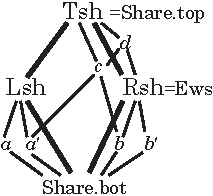
\includegraphics[scale=1.25]{graphics/shares.pdf}}

The \emph{top} share, written \lstinline{Tsh} or
\lstinline{Share.top}, gives total permission: to deallocate any cells
within the footprint of this mapsto, to read, to write.
\[
\begin{array}{ll}
\mathsf{Share.split}~\mathsf{Tsh} = (\mathsf{Lsh},\mathsf{Rsh}) & \\
\mathsf{Share.split}~\mathsf{Lsh} = (a,a')  & \mathsf{Share.split}~\mathsf{Rsh} = (b,b') \\
a'\oplus b = c & \mathrm{lub}(c,\mathsf{Rsh})=a'\oplus \mathsf{Rsh}=d\\
\multicolumn{2}{l}{\forall \mathit{sh}.~\mathsf{writable\_share}~\mathit{sh}~\rightarrow~\mathsf{readable\_share}~\mathit{sh}}\\
\mathsf{writable\_share}~\mathsf{Ews} & \mathsf{readable\_share}~\mathsf{b} \\
\mathsf{writable\_share}~d & \mathsf{readable\_share}~c \\
\mathsf{writable\_share}~\mathsf{Tsh} &  \neg \mathsf{readable\_share}~\mathsf{Lsh} \\
\end{array}
\]
Any share may be split into a \emph{left half} and a \emph{right half}.
The left and right of the top share are given distinguished names
\lstinline{Lsh, Rsh}.

The right-half share of the top share (or any share containing it such
as $d$) is sufficient to grant \emph{write permission} to the data:
``the right share is the write share.''  A thread of execution holding
only \lstinline{Lsh}---or subshares of it such as $a,a'$---can neither
read or write the object, but such shares are not completely useless:
holding any nonempty share prevents other threads from deallocating
the object.

Any subshare of \lstinline{Rsh}, in fact any share that overlaps
 \lstinline{Rsh}, grants \emph{read} permission to the object.
Overlap can be tested using the glb (greatest lower bound) operator.

Whenever \lstinline{(mapsto $\mathit{sh}$ t v w)} holds, then the share $\mathit{sh}$
must include at least a read share, thus this give permission to load
memory at address $v$ to get a value $w$ of type $t$.

To make sure $\mathit{sh}$ has enough permission to write (i.e., 
$\mathsf{Rsh} \subset \mathit{sh}$, we can say \lstinline{writable_share $\mathit{sh}$ : Prop}.

Memory obtained from \lstinline{malloc} comes with the top share
\lstinline{Tsh}.  Writable extern global variables
and stack-allocated addressable locals (which of course
must not be deallocated) come with the ``extern writable share'' 
\lstinline{Ews} which is equal to \lstinline{Rsh}.
Read-only globals come with a half-share of \lstinline{Rsh}.

Sequential programs usually have little need of any shares except
the \lstinline{Tsh} and \lstinline{Ews}.  However, many function 
specifications can be parameterized over any share (example: \autopageref{refcard:example-readable-share}), and this sort
of generalized specification makes the functions usable in more contexts.

In C it is undefined to test deallocated pointers for equality or inequalities,
so the Hoare-logic rule for pointer comparison also requires some
permission-share; see \autopageref{refcard:pointer-cmp}.


\chapter{Pointer comparisons}

\chapter{Proving larg(ish) programs}

When your program is not all in one .c file,
see also \autoref{refcard:sepcomp}.
Whether or not your program is all in one .c file,
you can prove the individual function bodies in separate .v files.
This uses less memory, and (on a multicore computer with
parallel \lstinline{make}) saves time.
To do this, put your API spec (up to the construction
of \lstinline{Gprog} in one file;
then each \lstinline{semax_body} proof in a separate file
that imports the API spec.

\subsection{Extraction of subordinate semax-goals}
To ease memory pressure and recompilation time, it is often advisable
to partition the proof of a function into several lemmas. Any proof
state whose goal is a semax-term can be extracted as a stand-alone
statement by invoking tactic $\mathit{semax\_subcommand}\ V\ G\ F$.
The three arguments are as in the statement of surrounding semax-body
lemma, i.e.~are of type $\mathit{varspecs}$, $\mathit{funspecs}$, and
$\mathit{function}$. 

The subordinate tactic $\mathit{mkConciseDelta}\ V\ G\ F\ \mathit{Delta}$ can
also be invoked individually, to simply display the type context Delta
in consise form, as the application of a sequence of initializations
to the host function's func\_tycontext.

\subsection{The freezer}
A distinguishing feature of separation logic is the frame rule,
i.e.~the ability to modularly verify a statement w.r.t.~its minimal
resource footprint. Unfortunately, being phrased in terms of the
syntatic program structure, the standard frame rule does not easily
interact with forward symbolic execution as implemented by the Floyd
tactics (and many other systems), as these continuously rearrange the
associativity of statement sqeuencing to peel off the redex of the
next \emph{forward}, and (purposely) hide the program continuation as
the abbreviation \emph{MORE\_COMMANDS}. 

Resolving this conflict, Floyd's \emph{freezer} abstraction provides a
means for flexible framing, by implementing a veil that opaquely hides
selected items of a SEP clause from non-symbolic treatment by
non-freezer tactics.

The freezer abstraction consists of two main tactics, $\mathit{freeze}\
N\ F$ and $\mathit{thaw}\ F$, where $N:\mathit{list\ nat}$ and $F$ is
a user-supplied (fresh) Coq name. The result of applying
$\mathit{freeze}\ [i_1;\ldots;i_n]\ F$ to a semax goal is to remove
items $i_1,\ldots,i_n$ from the precondition's SEP clause, inserting
the item $\mathit{FRZL}\ F$ at the head of the SEP list, and adding a
hypothesis $F := \mathit{abbreviate}$ to Coq's proof context.

The term $\mathit{FRZL}\ F$ participates symbolically in all
non-freezer tactics just like any other SEP item, so can in particular
be canceled, and included in a function call's frame.  Unfolding a
freezer is not tied to the associativity structure of program
statements but can be achieved by invoking $\mathit{thaw}\ F$, which
simply replaces $\mathit{FRZL}\ F$ by the the list of $F$'s
constiuents.  As multiple freezers can coexists and freezers can be
arbitrarily nested, SEP-clauses $R$ effectively contain forests of
freezers, each constituent being thawable independently and
freezer-level by freezer-level.

Wrapping single \emph{forward} or \emph{forward\_call} commands in a
freezer often speeds up the processing time noticably, as invocations
of subordinate tactics \emph{entailer}, \emph{cancel}, etc.~are
supplied with smaller and more symbolic proof goals. In our
experience, applying the freezer throughout the proof of an entire
function body typically yields a speedup of about 30\% on average with
improvements of up to 55\% in some cases, while also easing the memory
pressure and freeing up valuable real estate on the user's screen.


A more invasive implementation of a freezer-like abstraction would
refine the \lstinline{PROP($P$) LOCAL($Q$) SEP($R$)} structure to
terms of the form \lstinline{PROP($P$) LOCAL($Q$) SEP($R$) FR($H$)}
where $H: \emph{list\ mpred}$. Again, terms in $H$ would be treated
opaquely by all tactics, and freezing/thawing would correspond to
transfer rules between $R$ and $H$. In either case, forward symbolic
execution is reconciled with the frame rule, and the use of the
mechanism is sound engineering practice as documentation of
programmer's insight is combined with performance improvements.

\chapter{Separate compilation, \upshape\textsf{semax\_ext}}
\label{refcard:sepcomp}

What to do when your program is spread over multiple .c files.

\subsection{Code preparation}
In order to separate the namespaces of multiple files compiled by CompCert's clightgen tool, it is necessary to apply

python fix\_clightgen.py file1.v ...fileN.v

The script reads in the named files, concisely renames variables etc by
making up new positives, and writes the modified files back to the
given names.



\chapter{Appendix: catalog of major tactics/commands}
Below is an alphabetic catalog of the major floyd tactics. In addition
to short descriptions, the entries indicate whether a tactic (or
tactic notation) is typically user-applied [u], primarily of
internal use [i] or is expected to be used at development-time
but unlikely to appear in a finished proof script [d]. We also
mention major interdependencies between tactics, and their points of
definition.

\paragraph{[ui] andp\_left2}

Used frequently in combination with \emph{derives\_refl} to clean up
proofs states at the end of a loop or function, or after a \emph{forward\_seq}.\\
Subordinate tactics: \ldots\\
Superordinate tactics: \ldots\\
Defined in XXX.v

\paragraph{[u] cancel}
Main vehicle for resolving entailments between mpred lists.  Performs
symbolic cancellation, i.e.~performs little inspection of the
internals of mpreds. May turn a provable goal into an unprovable goal,
by cancelling too aggressively. Occasionally needs to be finished off
with a \emph{derives\_refl}, in case of syntatically not mtaching
compspecs\footnote{Do these cases still occur? Any other cases?}.

Subordinate tactics: \ldots\\
Superordinate tactics: \ldots\\
Defined in XXX.v

\paragraph{[u] derives\_refl'}
(Actually, a lemma, not a tactic). Often followed by
$\mathit{f_equal}$ to solve, say, an entailment between two almost
identical $\mathit{data\_at}$ predicates.

\paragraph{[u] entailer}

Vehicle for proving entailments at the mpred level or the assertion
level\ldots\\
Say sth about (non-)inclusion of saturate\_locals, normalize, cancel?\\
Subordinate tactics: \ldots\\
Superordinate tactics: \ldots\\
Defined in  XXX.v\\


\paragraph{[ui] derives\_refl and derives\_refl'}

Subordinate tactics: \ldots\\
Superordinate tactics: \ldots\\
Defined in XXX.v

\paragraph{[u] drop\_LOCAL n}
where $n:nat$. Removes the $n$th entry of a the LOCAL block of a
semax\_statement's precondition\footnote{or of an assertion-level
  entailment's LHS?}.

Subordinate tactics: \ldots\\
Superordinate tactics: \ldots\\
Defined in XXX.v

\paragraph{[u] entailer!}

Vehicle for proving entailments at the mpred level or the assertion
level\ldots
In contrast to \emph{entailer}, \emph{entailer!} may turn a provable
entailment into an unprovable one, but is usually more efficient.\\
Say sth about (non-)inclusion of saturate\_locals, normalize, cancel?\\
Subordinate tactics: \ldots\\
Superordinate tactics: \ldots\\
Defined in  XXX.v

\paragraph{[u] forward}

Subordinate tactics: \ldots\\
Superordinate tactics: \ldots\\
Defined in XXX.

\paragraph{[u] forward\_call ARGS}
Tactic for stepping through the call to a specified function, where
\emph{ARGS} is the product of arguments, i.e.~an in-order
instantiation of the function specification's WITH clause (Note:
little type checking is applied to \emph{ARGS} and the tactic may
behave erratically if incorrect/wrongly-typed arguments are supplied).

Always leaves a \emph{semax}-subgoal for the program
continuation.  Frequently, leaves an entailment subgoal for
establishing the function procondition, and/or a subgoal for a typing
side condition.

Subordinate tactics: \ldots\\
Superordinate tactics: None.\\
Defined in XXX.v, with the underlying proof rules being defined in YYY.v

\paragraph{[u] forward\_for}

Including its variants for simple bounds etc

Is expected to leave the following subgoals:\ldots

Subordinate tactics: \ldots\\
Superordinate tactics: \ldots\\
Defined in XXX


\paragraph{[u] forward\_seq}

Subordinate tactics: \ldots\\
Superordinate tactics: \ldots\\
Defined in XXX.

\paragraph{[i] mkConciseDelta\ V\ G\ F\ Delta}
Applicable to a proof state with a semax goal. Simplies the $\Delta$
component to the application of a sequence of initializations to the
host function's func\_tycontext.

Superordinate tactics:  $\mathit{semax\_subcommand}$\\
Defined in semax\_tactics.v. 

\paragraph{[u] semax\_subcommand\ V\ G\ F}
Applicable to a proof state with a semax goal.
Extracts the current proof state as a stand-alone
statement that can be copy-and pasted to a separate file.
The three arguments are as in the statement of surrounding semax-body
lemma, i.e.~are of type $\mathit{varspecs}$, $\mathit{funspecs}$, and
$\mathit{function}$. 

Subordinate tactic: $\mathit{mkConciseDelta}$.
Defined in semax\_tactics.v. 



\chapter{BOUNDARY}
Everything beyond here is junk, left over from the
old Verifiable C manual, that needs to be rewritten and moved
above the boundary.

\chapter{Getting started}

This \emph{summary reference manual} 
is a brief guide to the
VST Separation Logic for the C language.
The Verified Software Toolchain and
the principles of its program logics
are described in the book:

\noindent \emph{\large Program Logics for Certified Compilers,}\newline
by Andrew W. Appel \emph{et al.},
Cambridge University Press, 2014.  
\vspace{-2ex}

\newthought{To install the VST Separation Logic for C light:}
\begin{enumerate}\setlength\itemsep{0pt}
\item  Get VST from \textsf{vst.cs.princeton.edu/download},
or get the bleeding-edge version from 
\textsf{https://github.com/PrincetonUniversity/VST}.
\item Examine \lstinline{vst/compcert/VERSION} to determine which
version of CompCert to download.
The VST comes with a copy of the CompCert front-end, in vst/compcert/,
but (at present) CompCert's \iref{clightgen} utility is not buildable
from just the front-end distributed with VST.  You'll need \iref{clightgen}
to translate .c files into .v files containing C light abstract syntax.
Thus it's recommended to download
and build CompCert.

\item Get CompCert from \textsf{compcert.inria.fr/download.html}
and run \textsf{./configure} to list configurations. Select the correct option
for your machine, then run \textsf{./configure <option>} followed by \newline
\textsf{make clightgen}.
Create a file \lstinline{vst/CONFIGURE} containing a definition for CompCert's location;
if vst and CompCert are installed in the same
parent directly, use \lstinline{COMPCERT=../compcert}

If you have  not installed CompCert,
use the CompCert front-end packaged with VST.
Do not create a CONFIGURE file, and do:\newline
\lstinline{cd vst/compcert; ./make}  

\item In the \lstinline{vst} directory, \lstinline{make}.
\end{enumerate}
See also the file \file{vst/BUILD\_ORGANIZATION}.


The \lstinline{verif_reverse.v} example is described
in PLCC \autoref{ch:clight-program}.
You might find it interesting to open this in the IDE,
using the command shown above,
and interactively step through the definitions and proofs.

Before doing proofs of your own, you may find it helpful
to step through this tutorial on C light expressions and
assertions:\newline
\lstinline{cd examples/floyd_tut; coqide tutorial.v}\newline
(this tutorial sets up its own load paths.)

\ychapter{Differences from PLCC}{}
The book \emph{Program Logics for Certified Compilers}
(Cambridge University Press, early 2014) describes
\emph{Verifiable C} version 1.1.  
More recent VST versions differ in the following ways
from what the PLCC book describes:
\begin{itemize}
\item In the $\LOCAL$ component of an assertion, \newline
\lstinline{temp $i$ $v$}~ is the recommended
way to write ~\lstinline{`(eq $v$) (eval_id $i$)}, 
and \newline
\lstinline{var $i$ $t$ $v$}~ is the recommended
way to write ~\lstinline{`(eq $v$) (eval_var $i$ $t$)}.
See \autoref{refcard:supercanonical} of this manual.
\item The type-checker now has a more refined view of char and short types
     (see \autoref{refcard:tcval} of this manual).
\item \lstinline{field_mapsto} is now called
\lstinline{field_at}, and it is dependently
typed; see \autoref{refcard:structured} of this manual.
\item \lstinline{typed_mapsto} is renamed to \lstinline{data_at}, and
   last two arguments are swapped.
\item \lstinline{umapsto} (``untyped mapsto'') no
longer exists.
\item \lstinline{mapsto $\mathit{sh}$ $t$ $v$ $w$}
~~~now permits either ($w=$\lstinline{Vundef})
or the value $w$ belongs to type $t$.  
This permits describing uninitialized locations,
i.e., \lstinline{mapsto_ $\mathit{sh}$ $t$ $v$ = mapsto_ $\mathit{sh}$ $t$ $v$ Vundef}.
See \autoref{refcard:structured} of this manual.
\item Supercanonical form is now suggested; see 
\autoref{refcard:supercanonical} of this manual.
\item For function calls, do not use \lstinline{forward}
(except to get advice about the witness type);
instead, use \lstinline{forward_call}.  See \autopageref{forward-call}.
\item C functions may now fall through the end of the function body,
and this is (per the C semantics) equivalent to a \lstinline{return;}
statement.
\end{itemize}
\ychapter{Memory predicates}{}

The axiomatic semantics (Hoare Logic of Separation) treats
memories abstractly.  One never has a variable $m$ of type
\emph{memory}.  Instead, one uses the Hoare Logic to manipulate
predicates $P$ on memories.  
Our type of ``memory predicates'' is called \lstinline{mpred}

Although intuitively $\mathsf{mpred}$
``feels like'' the type $\mathsf{memory}\rightarrow\mathsf{Prop}$,
the underlying semantic model is different;
thus we keep the type \lstinline{mpred} abstract (opaque).
See \emph{Program Logics for Certified Compilers (PLCC)} 
for more explanation.

On the type \lstinline{mpred}
we form a natural deduction  system 
\lstinline{NatDed(mpred)} with 
conjuction $\andp$, disjunction $\orp$, etc.;
a separation logic 
\lstinline{SepLog(mpred)} with 
separating conjunction $*$ and \lstinline{emp};
and an indirection theory 
\lstinline{Indir(mpred)} with $\later$ ``later.''

The natural deduction system has a sequent
(entailment) operator written \lstinline{P |$$-$$- Q} in Coq
(written $P\vdash Q$ in print), where $P,Q:\mathsf{mpred}$.  We write
bientailment simply as $P=Q$ since we
assume axioms of extensionality.




\ychapter{Separation Logic}{(see PLCC \autoref{ch:logic})}
\begin{lstlisting}
Class NatDed (A: Type) := mkNatDed {
  andp: A -> A -> A;  $\qquad$(Notation $\andp$)
  orp: A -> A -> A;   $\qquad$(Notation $\orp$)
  exp: forall {T:Type}, (T -> A) -> A;    $\qquad$(Notation EX)
  allp: forall {T:Type}, (T -> A) -> A;   $\qquad$(Notation ALL)
  imp: A -> A -> A;   $\qquad$(Notation -$$-$$>, here written --> )
  prop: Prop -> A;    $\qquad$(Notation !! )
  derives: A -> A -> Prop;  $\qquad$(Notation |$$-$$-, here written |-- )
  pred_ext: forall P Q, P|--Q -> Q|--P -> P=Q;
  derives_refl: forall P,  P |-- P;
  derives_trans: forall {P Q R}, P |-- Q -> Q |-- R -> P|--R;
  TT := !!True;
  FF := !!False;
  andp_right:  forall X P Q:A, X|--P -> X|--Q ->  X|--(P&&Q);
  andp_left1:  forall P Q R:A, P|--R -> P&&Q |-- R;
  andp_left2:  forall P Q R:A, Q|--R -> P&&Q |-- R;
  orp_left: forall P Q R, P|--R -> Q|--R -> $~$ P||Q |--R;
  orp_right1: forall P Q R, P|--Q -> P|-- Q||R;
  orp_right2: forall P Q R, P|--R -> P|-- Q||R;
  exp_right: forall {B: Type}(x:B)(P:A)(Q: B->A), P|--Q x -> P|-- EX x:B, Q;
  exp_left: forall{B: Type}(P:B->A)(Q:A), (forall x, P x |-- Q) -> EX x:B,P |-- Q;
  allp_left: forall {B}(P: B -> A) x Q, P x|--Q -> ALL x:B,P|--Q;
  allp_right: forall{B}(P: A)(Q:B->A), (forall v, P|-- Q v) -> P|-- ALL x:B,Q;
  imp_andp_adjoint: forall P Q R, P&&Q|--R $$ <-> $$ $$ P|--(Q-->R);
  prop_left: forall (P: Prop) Q, (P -> (TT|--Q)) -> !!P |-- Q;
  prop_right: forall (P: Prop) Q, P -> (Q|-- !!P);
  not_prop_right: forall(P:A)(Q:Prop), (Q -> (P|--FF))-> P|--!!(~Q)
}.
\end{lstlisting}

\clearpage
\begin{lstlisting}
Class SepLog (A: Type) {ND: NatDed A} := mkSepLog {
  emp: A;
  sepcon: A -> A -> A;   $\qquad$(Notation * )
  wand: A -> A -> A;     $\qquad$(Notation -*; here written $\wand$ )
  ewand: A -> A -> A;    $\qquad$(no notation; here written $\ewand$ )
  sepcon_assoc: forall P Q R, (P*Q)*R = P*(Q*R);
  sepcon_comm:  forall P Q, P*Q = Q*P;
  wand_sepcon_adjoint: forall (P Q R: A),  P*Q|--R $$ <-> P |-- Q$\wand$R;
  sepcon_andp_prop: forall P Q R, P*(!!Q && R) = !!Q && (P*R);
  sepcon_derives: forall P P' Q Q' : A, P|--P' -> Q|--Q' -> P*Q |-- P'*Q';
  ewand_sepcon: forall (P Q R : A),  (P*Q)$\ewand$ R = P $\ewand$ (Q $\ewand$ R);
  ewand_TT_sepcon: forall (P Q R: A),
       (P*Q)&&(R$\ewand$TT) |-- (P &&(R$\ewand$TT))*(Q && (R$\ewand$TT));
  exclude_elsewhere: forall P Q: A, P*Q |-- (P &&(Q$\ewand$  TT))*Q;
  ewand_conflict: forall P Q R, P*Q|--FF $$ -> $$ P&&(Q$\ewand$  R) |-- FF
}.
Class Indir (A: Type) {ND: NatDed A} := mkIndir {
  later: A -> A;   (Notation |> )
  now_later: forall P: A, P |-- |>P;
  later_K: forall P Q, |>(P-->Q) |-- (|>P --> |>Q);
  later_allp: forall T (F: T->A),  |>(ALL x:T, F x) = ALL x:T, |>(F x);
  later_exp: forall T (F: T->A), EX x:T, |>(F x) |-- |>(EX x: F x);
  later_exp': forall T (any:T) F, |>(EX x: F x) $$ = $$ EX x:T, |>(F x);
  later_imp: forall P Q,  |>(P-->Q) $$ $$ = $$ $$ (|>P --> |>Q);
  loeb: forall P,   |>P |-- P ->  TT |-- P
}.
Class SepIndir (A: Type) {NA: NatDed A}{SA: SepLog A}{IA: Indir A} := 
 mkSepIndir {
  later_sepcon: forall P Q, |>(P * Q) = |>P * |>Q;
  later_wand: forall P Q, |>(P $\wand$ Q) = |>P $\wand$ |>Q;
  later_ewand: forall P Q, |>(P $\ewand$ Q) = (|>P) $\ewand$ (|>Q)
}.
\end{lstlisting}
\vspace*{-24pt}
\ychapter{Mapsto and func\_ptr}{(see PLCC \autoref{clight-mapsto})}

Aside from the standard operators and axioms of separation logic,
we have exactly two primitive
memory predicates:

\begin{lstlisting}
Parameter address_mapsto: 
    memory_chunk -> val -> share -> share -> address -> mpred.
Parameter func_ptr : funspec -> val ->mpred.
\end{lstlisting}
\lstinline{func_ptr $\phi$ v} $\qquad$ means that value $v$
is a pointer to a function with specification $\phi$.

\lstinline{address_mapsto} expresses what is typically
written $x\mapsto y$ in separation logic,
that is, a singleton heap containing just value $y$ at address $x$.
But we almost always use one of the following derived forms:

\noindent \lstinline{mapsto ($\mathit{sh}$:share) (t:type) (v w: val) : mpred}
$\qquad$describes a singleton heap with
just one value $w$ of (C-language) type $t$
at address $v$, with permission-share $\mathit{sh}$.

\noindent \lstinline{mapsto_ $$ ($\mathit{sh}$:share) (t:type) (v:val) : mpred}
$\qquad$
describes an \emph{uninitialized} singleton heap with
space to hold a value of type $t$
at address $v$, with permission-share $\mathit{sh}$.

\noindent
\lstinline{field_at ($\mathit{sh}$: share) (t: type) (f: list ident) (w: reptype (nested\_field\_type2 f) (v: val) : mpred}
\newline  describes a heap
that holds just field \lstinline{fld} 
of \lstinline{struct}-value $v$,
belonging to \lstinline{struct}-type $t$, 
containing value $w$.
If type $t$ describes a nested \lstinline{struct} type,
then $f$ can actually be a path of field selections
that descends into the nested structures.
If $f$ is the empty path, then the field is equivalent to
\lstinline{data_at}.
The type of $w$ is a dependent type.
\emph{Note: arguments $w,v$ are swapped compared to the PLCC book.}

\lstinline{field_at_ ($\mathit{sh}$: share) (t: type) (fld: ident) (v: val) : mpred}
\newline is the corresponding uninitialized structure-field.


\ychapter{CompCert C}{}

The CompCert verified C compiler translates standard C source programs
into an abstract syntax for \emph{CompCert C},
and then translates that into abstract syntax
for \emph{C light}.  
Then VST Separation Logic is applied to the C light abstract syntax.
C light programs proved correct using the VST separation logic
can then be compiled (by CompCert) to assembly language.

C light syntax is defined by these Coq files from CompCert:

\begin{description}
\item[Integers.]  32-bit (and 8-bit, 16-bit, 64-bit) signed/unsigned integers.
\item[Floats.]  IEEE floating point numbers.
\item[Values.]  The \lstinline|val| type: integer + float + pointer + undefined.
\item[AST.]  Generic support for abstract syntax.
\item[Ctypes.]  C-language types and structure-field-offset computations.
\item[Cop.]  Semantics of C-language arithmetic operators.
\item[Clight.]  Abstract syntax of C-light expressions, statements, and functions.
\item[veric.expr.]  (from VST, not CompCert) Semantics of expression evaluation.
\end{description}

Some of the important types and operators are described over the next 
few pages.

\ychapter{Verifiable C programming}{See PLCC Chapter \ref{ch:compcert-intro}}
\label{refcard:verifiable-c}
In writing Verifiable C programs you must:

\begin{itemize}
  \item Make each dereference into a top level expression (PLCC
  \autopageref{verifiable-c})
  \item Make most pointer comparisons into a top level expression (PLCC
  \autopageref{pointercompare})
  \item Remove casts between \lstinline|int| and pointer types (result in
  values that crash if used)
\end{itemize}

The \lstinline{clightgen} tool automatically:

\begin{itemize}
  \item Factors function calls into top level expressions
  \item Factors logical \lstinline{and}/\lstinline{or} operators into 
\lstinline{if} statements (to capture
  short circuiting behavior)
\end{itemize}

Proof automation detects these two transformations and processes them with a
single tactic application.

If your program uses \lstinline|malloc| or \lstinline|free|, you must declare
and specify these as external functions. If you don't want to keep track of the
size of each allocated object, you may want to change the interface of the
\lstinline|free| function. We do this in our example definitions of
\lstinline|malloc| and \lstinline|free| in \file{progs/queue.c} and their
specifications in \file{progs/verif\_queue.v}.

\ychapter{32-bit Integers}{(\file{compcert/lib/Integers.v})}

The VST program logic uses CompCert's 32-bit integer type.

\begin{lstlisting}
Inductive comparison := Ceq | Cne | Clt | Cle | Cgt | Cge.
Definition wordsize: nat := 32.  (* also instantiations for 8, 16, 64 *)
Definition modulus : Z := two_power_nat wordsize.
Definition half_modulus : Z := modulus / 2.
Definition max_unsigned : Z := modulus - 1.
Definition max_signed : Z := half_modulus - 1.
Definition min_signed : Z := - half_modulus.

Parameter int : Type.
Parameter unsigned : int -> Z.
Parameter signed : int -> Z.
Parameter repr : Z -> int.

Definition zero := repr 0.

Definition eq (x y: int) : bool.
Definition lt (x y: int) : bool.
Definition ltu (x y: int) : bool.
Definition neg (x: int): int := repr (- unsigned x).
Definition add (x y: int): int :=  repr (unsigned x + unsigned y).
Definition sub (x y: int): int :=  repr (unsigned x - unsigned y).
Definition mul (x y: int): int :=  repr (unsigned x * unsigned y).
Definition divs (x y: int) : int.
Definition mods (x y: int) : int.
Definition divu (x y: int) : int.
Definition modu (x y: int) : int.
Definition and (x y: int): int := bitwise_binop andb x y.
Definition or (x y: int): int := bitwise_binop orb x y.
Definition xor (x y: int) : int := bitwise_binop xorb x y.
Definition not (x: int) : int := xor x mone.
Definition shl (x y: int): int.
Definition shru (x y: int): int.
Definition shr (x y: int): int.
Definition rol (x y: int) : int.
Definition ror (x y: int) : int.
Definition rolm (x a m: int): int.
Definition cmp (c: comparison) (x y: int) : bool.
Definition cmpu (c: comparison) (x y: int) : bool.

Lemma eq_dec: forall (x y: int), {x = y} + {x <> y}.
Theorem unsigned_range: forall i, 0 <= unsigned i < modulus.
Theorem unsigned_range_2:  forall i, 0 <= unsigned i <= max_unsigned.
Theorem signed_range:  forall i, min_signed <= signed i <= max_signed.
Theorem repr_unsigned:  forall i, repr (unsigned i) = i.
Lemma repr_signed:  forall i, repr (signed i) = i.
Theorem unsigned_repr: 
   forall z, 0 <= z <= max_unsigned -> unsigned (repr z) = z.
Theorem signed_repr:
  forall z, min_signed <= z <= max_signed -> signed (repr z) = z.
Theorem signed_eq_unsigned:
  forall x, unsigned x <= max_signed -> signed x = unsigned x.

Theorem unsigned_zero: unsigned zero = 0.
Theorem unsigned_one: unsigned one = 1.
Theorem signed_zero: signed zero = 0.

Theorem eq_sym:  forall x y, eq x y = eq y x.
Theorem eq_spec: forall (x y: int), if eq x y then x = y else x <> y.
Theorem eq_true: forall x, eq x x = true.
Theorem eq_false: forall x y, x <> y -> eq x y = false.

Theorem add_unsigned: forall x y, add x y = repr (unsigned x + unsigned y).
Theorem add_signed: forall x y, add x y = repr (signed x + signed y).
Theorem add_commut: forall x y, add x y = add y x.
Theorem add_zero: forall x, add x zero = x.
Theorem add_zero_l: forall x, add zero x = x.
Theorem add_assoc: forall x y z, add (add x y) z = add x (add y z).

Theorem neg_repr: forall z, neg (repr z) = repr (-z).
Theorem neg_zero: neg zero = zero.
Theorem neg_involutive: forall x, neg (neg x) = x.
Theorem neg_add_distr: forall x y, neg(add x y) = add (neg x) (neg y).

Theorem sub_zero_l: forall x, sub x zero = x.
Theorem sub_zero_r: forall x, sub zero x = neg x.
Theorem sub_add_opp: forall x y, sub x y = add x (neg y).
Theorem sub_idem: forall x, sub x x = zero.
Theorem sub_add_l: forall x y z, sub (add x y) z = add (sub x z) y.
Theorem sub_add_r: forall x y z, sub x (add y z) = add (sub x z) (neg y).
Theorem sub_shifted: forall x y z, sub (add x z) (add y z) = sub x y.
Theorem sub_signed:  forall x y, sub x y = repr (signed x - signed y).

Theorem mul_commut: forall x y, mul x y = mul y x.
Theorem mul_zero: forall x, mul x zero = zero.
Theorem mul_one: forall x, mul x one = x.
Theorem mul_assoc: forall x y z, mul (mul x y) z = mul x (mul y z).
Theorem mul_add_distr_l: forall x y z, mul (add x y) z = add (mul x z) (mul y z).
Theorem mul_signed: forall x y, mul x y = repr (signed x * signed y).
\end{lstlisting}
and many more axioms for the bitwise operators, shift operators,
signed/unsigned division and mod operators.



\ychapter{C expression syntax}{(\file{compcert/cfrontend/Clight.v})}

\begin{lstlisting}
Inductive expr : Type :=
(* 1$~$  *) $~~~$   | Econst_int: int -> type -> expr      
(* 1.0 *)   $~$ | Econst_float: float -> type -> expr  (* double precision *)
(* 1.0f0 *)    | Econst_single: float -> type -> expr (* single precision *)
(* 1L  *)  $~~$  | Econst_long: int64 -> type -> expr
(* x   *) $~~~~$   | Evar: ident -> type -> expr         
(* x   *) $~~~~$   | Etempvar: ident -> type -> expr     
(* *e  *) $~~~$   | Ederef: expr -> type -> expr        
(* &e  *) $~~$   | Eaddrof: expr -> type -> expr       
(* ~e  *) $~~$   | Eunop: unary_operation -> expr -> type -> expr
(* e+e *) $~$   | Ebinop: binary_operation -> expr -> expr -> type -> expr 
(* (int)e *) | Ecast: expr -> type -> expr  
(* e.f *) $~~$ | Efield: expr -> ident -> type -> expr. 

Definition typeof (e: expr) : type :=
  match e with
  | Econst_int _ ty => ty
  | Econst_float _ ty => ty
  | Evar _ ty => ty
  | ... $et~cetera$.
\end{lstlisting}

\ychapter{C operators}{(\file{compcert/cfrontend/Cop.v})}
\begin{lstlisting}

Function bool_val (v: val) (t: type) : option bool :=
  match classify_bool t with
  | bool_case_i =>
      match v with
      | Vint n => Some (negb (Int.eq n Int.zero))
      | _ $$ => None
      end
  | bool_case_f =>
      match v with
      | Vfloat f => Some (negb (Float.cmp Ceq f Float.zero))
      | _ $$ => None
      end
  | bool_case_p =>
      match v with
      | Vint n => Some (negb (Int.eq n Int.zero))
      | Vptr b ofs => Some true
      | _ $$ => None
      end
  | bool_default => None
  end.

Function sem_neg (v: val) (ty: type) : option val :=
  match classify_neg ty with
  | neg_case_i sg =>
      match v with
      | Vint n => Some (Vint (Int.neg n))
      | _ $$ => None
      end
  | neg_case_f =>
      match v with
      | Vfloat f => Some (Vfloat (Float.neg f))
      | _ $$ => None
      end
  | neg_default => None
  end.

Function sem_add (v1:val) (t1:type) (v2: val) (t2:type) : option val :=
  match classify_add t1 t2 with 
  | add_case_ii sg =>                   (**r integer addition *)
      match v1, v2 with
      | Vint n1, Vint n2 => Some (Vint (Int.add n1 n2))
      | _,  _ $$ => None
      end
  | add_case_ff =>                      (**r float addition *)
      match v1, v2 with
      | Vfloat n1, Vfloat n2 => Some (Vfloat (Float.add n1 n2))
      | _,  _ $$ => None
      end
  | add_case_if sg =>                   (**r int plus float *)
      match v1, v2 with
      | Vint n1, Vfloat n2 => Some (Vfloat (Float.add (cast_int_float sg n1) n2))
      | _, _ $$ => None
      end
  | ... $(cases~omitted)$
  | add_case_ip ty _ $$ =>                 (**r integer plus pointer *)
      match v1,v2 with
      | Vint n1, Vptr b2 ofs2 => 
        Some (Vptr b2 (Int.add ofs2 (Int.mul (Int.repr (sizeof ty)) n1)))
      | _,  _ $$ => None
      end   
  | add_default => None
end.

Function sem_sub (v1:val) (t1:type) (v2: val) (t2:type) : option val.
Function sem_mul (v1:val) (t1:type) (v2: val) (t2:type) : option val.
Function sem_div (v1:val) (t1:type) (v2: val) (t2:type) : option val.
Function sem_mod (v1:val) (t1:type) (v2: val) (t2:type) : option val.
Function sem_and (v1:val) (t1:type) (v2: val) (t2:type) : option val.

Function sem_cmp (c:comparison)
                  (v1: val) (t1: type) (v2: val) (t2: type)
                  (m: mem): option val :=
  match classify_cmp t1 t2 with
  | cmp_case_ii Signed =>
      match v1,v2 with
      | Vint n1, Vint n2 => Some (Val.of_bool (Int.cmp c n1 n2))
      | _,  _ $$ => None
      end
  | ... $(many~more~cases~)$
  end.

Definition sem_binary_operation
    (op: binary_operation)
    (v1: val) (t1: type) (v2: val) (t2:type)
    (m: mem): option val :=
  match op with
  | Oadd => sem_add v1 t1 v2 t2
  | Osub => sem_sub v1 t1 v2 t2 
  | Omul => sem_mul v1 t1 v2 t2
  | Omod => sem_mod v1 t1 v2 t2
  | Odiv => sem_div v1 t1 v2 t2 
  | Oand => sem_and v1 t1 v2 t2
  | Oor  => sem_or v1 t1 v2 t2
  | Oxor  => sem_xor v1 t1 v2 t2
  | Oshl => sem_shl v1 t1 v2 t2
  | Oshr  => sem_shr v1 t1 v2 t2   
  | Oeq => sem_cmp Ceq v1 t1 v2 t2 m
  | One => sem_cmp Cne v1 t1 v2 t2 m
  | Olt => sem_cmp Clt v1 t1 v2 t2 m
  | Ogt => sem_cmp Cgt v1 t1 v2 t2 m
  | Ole => sem_cmp Cle v1 t1 v2 t2 m
  | Oge => sem_cmp Cge v1 t1 v2 t2 m
  end.
\end{lstlisting}

\ychapter{C expression evaluation}{(\file{vst/veric/expr.v})}

\begin{lstlisting}
Definition eval_id (id: ident) ($\rho$: environ).
  (* look up the tempory variable ``id'' in $\rho$ *)

Definition eval_cast (t t': type) (v: val) : val.
  (* cast value v from type t to type t', but beware! There are
     be $three$ types involved, if you include the native type of v. *)

Definition eval_unop (op: Cop.unary_operation) (t1 : type) (v1 : val) : val.

Definition eval_binop (op: Cop.binary_operation) 
               (t1 t2 : type) (v1 v2: val) : val.

Definition force_ptr (v: val) : val :=
       match v with Vptr l ofs => v | _ $$ => Vundef  end.

Definition eval_struct_field (delta: Z) (v: val) : val.
   (* offset the pointer-value v by delta *)

Definition eval_field (ty: type) (fld: ident) (v: val) : val.
   (* calculate the lvalue of (but do not fetch/dereference!)
      a structure/union field of value v *)

Definition eval_var (id:ident) (ty: type) (rho: environ) : val.
   (* Get the lvalue (address of) an addressable local variable
     (if there is one of that name) or else a global variable *)

Definition deref_noload (ty: type) (v: val) : val.
   (* For By_reference types such as arrays that dereference
      without actually fetching *)
 match access_mode ty with By_reference => v | _ $$ => Vundef end.
\end{lstlisting}

\clearpage
\begin{lstlisting}
Fixpoint eval_expr (e: expr) : environ -> val :=
 match e with
 | Econst_int i ty => `(Vint i)
 | Econst_float f ty => `(Vfloat f)
 | Etempvar id ty => eval_id id 
 | Eaddrof a ty => eval_lvalue a 
 | Eunop op a ty =>  `(eval_unop op (typeof a)) (eval_expr a) 
 | Ebinop op a1 a2 ty =>  
           `(eval_binop op (typeof a1) (typeof a2))
              (eval_expr a1) (eval_expr a2)
 | Ecast a ty => `(eval_cast (typeof a) ty) (eval_expr a) 
 | Evar id ty => `(deref_noload ty) (eval_var id ty)
 | Ederef a ty => `(deref_noload ty) (`force_ptr (eval_expr a))
 | Efield a i ty => `(deref_noload ty) 
                      (`(eval_field (typeof a) i) (eval_lvalue a))
 end

 with eval_lvalue (e: expr) : environ -> val := 
 match e with 
 | Evar id ty => eval_var id ty
 | Ederef a ty => `force_ptr (eval_expr a)
 | Efield a i ty => `(eval_field (typeof a) i) (eval_lvalue a)
 | _  => `Vundef
 end.
\end{lstlisting}

\ychapter{C type checking}{(See PLCC \autoref{ch:typecheck})}
Ideally, you will never notice the typechecker, but it may occasionally
generate side conditions that can not be solved automatically.
If you get a proof goal from the typechecker, it will be an entailment 
\lstinline!P |-- denote_tc_assert ($\ldots$)!. PLCC
\autoref{ch:clight-auto} discusses what you can do to solve these goals. 

If you are asked to prove an entailment where the typechecking condition
evaluates to \lstinline|False|, this may be because your program is not written in
Verifiable C. You may need to perform some local transformations on your C
program in order to proceed. We listed these transformations on
\autopageref{refcard:verifiable-c}. 

The type-context will always be visible in your proof in a line that looks like 
\lstinline|Delta := abbreviate : tycontext|. The \lstinline|abbreviate|
hides the implementation of the type context (which is generally large
and uninteresting). The
\lstinline|query_context| tactic shows the result of looking up a variable in
a typecontext. The tactic \lstinline|query_context Delta _p.| will add hypothesis
\lstinline|QUERY : (temp_types Delta) ! _p = Some (tptr t_struct_list, true)|.
This means that in \lstinline|Delta|, \lstinline|_p| is a temporary variable
with type \lstinline|tptr t_struct_list| and that it is known to be initialized.

\ychapter{Lifted separation logic}{(See PLCC \autoref{ch:lifted})}
Assertions in our Hoare triple of separation 
are presented as $\mathsf{env}\rightarrow
\mathsf{mpred}$, that is, functions from environment
to memory-predicate,
using our natural deduction system 
\lstinline{NatDed(mpred)} and separation logic
\lstinline{SepLog(mpred)}.

Given a separation logic over a type $B$ of formulas,
and an arbitrary type $A$, 
we can define a \emph{lifted} separation logic over functions $A \rightarrow B$.
The operations are simply lifted pointwise over the
elements of $A$.  Let $P,Q:~A\rightarrow B$,
let $R:T\rightarrow A \rightarrow B$ then define,
\[
\begin{array}{rccl}
(P \andp Q):& A\rightarrow B&:=& \mathrm{fun}~a~\Rightarrow~Pa \andp Qa\\
(P \orp Q):& A\rightarrow B&:=& \mathrm{fun}~a~\Rightarrow~Pa \orp Qa\\
(\exists x.R(x)):& A\rightarrow B&:=& \mathrm{fun}~a~\Rightarrow~\exists x.~Rxa\\
(\forall x.R(x)):& A\rightarrow B&:=& \mathrm{fun}~a~\Rightarrow~\forall x.~Rxa\\
(P \imp Q):& A\rightarrow B&:=& \mathrm{fun}~a~\Rightarrow~Pa \imp Qa\\
(P \vdash Q):& A\rightarrow B&:=& \forall a.~Pa \vdash Qa\\
(P * Q):& A\rightarrow B&:=& \mathrm{fun}~a~\Rightarrow~Pa * Qa\\
(P \wand Q):& A\rightarrow B&:=& \mathrm{fun}~a~\Rightarrow~Pa \wand Qa\\
\end{array}
\]
In Coq we formalize the typeclass instances
\lstinline{LiftNatDed},
\lstinline{LiftSepLog}, etc.,
as shown below.
For a type $B$, whenever \lstinline{NatDed B} and \lstinline{SepLog B} (and so on) have been defined, the lifted instances
\lstinline{NatDed (A->B)} and \lstinline{SepLog (A->B)} (and so on)
are automagically provided by the typeclass system.

\begin{lstlisting}
Instance LiftNatDed(A B: Type){ND: NatDed B}: NatDed (A->B):=
 mkNatDed (A -> B)
    (*andp*) (fun P Q x => andp (P x) (Q x))
    (*orp*) (fun P Q x => orp (P x) (Q x))
    (*exp*) (fun {T} (F: T -> A -> B) (a: A) => exp (fun x => F x a))
    (*allp*) (fun {T} (F: T -> A -> B) (a: A) => allp (fun x => F x a))
    (*imp*) (fun P Q x => imp (P x) (Q x))
    (*prop*) (fun P x => prop P)
    (*derives*) (fun P Q => forall x, derives (P x) (Q x))
     _ $$ _ $$ _ $$ _ $$ _ $$ _ $$ _ $$ _ $$ _ $$ _ $$ _ $$ _ $$ _ $$ _ $$ _ $$ _ $$ _ $$ _.

Instance LiftSepLog (A B: Type) {NB: NatDed B}{SB: SepLog B} 
      : SepLog (A -> B).
 apply (mkSepLog (A -> B) _ (fun $\rho$ => emp) 
            (fun P Q $\rho$ => P $\rho$ * Q $\rho$) (fun P Q $\rho$ => P $\rho$ -* Q $\rho$)).
 (* fill in proofs here *)
\end{lstlisting}

In particular, if $P$ and $Q$ are functions of type \lstinline{environ->mpred}
then we can write $P*Q$,  $P \andp Q$, and so on.

Consider this assertion:
\begin{lstlisting}
fun $\rho$ => mapsto $\mathit{sh}$ tint (eval_id _x $\rho$) (eval_id _y $\rho$) 
             * mapsto $\mathit{sh}$ tint (eval_id _u $\rho$) (Vint Int.zero)
\end{lstlisting}
which might appear as the precondition of a Hoare triple.
It represents $(x\mapsto y) *(u\mapsto 0)$ written in informal
separation logic, where $x,y,u$ are C-language variables
of integer type.
Because it can be inconvenient to manipulate explicit lambda expressions
and explicit environment variables $\rho$, we may write it in lifted
form,
\begin{lstlisting}
 `(mapsto $\mathit{sh}$ tint) (eval_id _x) (eval_id _y) 
* `(mapsto $\mathit{sh}$ tint) (eval_id _u) `(Vint Int.zero)
\end{lstlisting}
Each of the first two backquotes lifts a function
from type \lstinline{val->val->mpred} to type
\lstinline{(environ->val)->(environ->val)->(environ->mpred)},
and the third one lifts from \lstinline{val} to 
\lstinline{environ->val}.

\ychapter{Canonical forms}{(See PLCC \autoref{canonical-form})}
We write a \emph{canonical form} of an assertion as,
\[
\PROP(P_0;P_1;\ldots,P_{l-1})~
\LOCAL(Q_0;Q_1;\ldots,Q_{m-1})~
\SEP(R_0;R_1;\ldots,R_{n-1})
\]
The $P_i : \mathsf{Prop}$ are Coq propositions---these are independent
of the program variables and the memory.
The $Q_i : \mathsf{environ}->\mathsf{Prop}$ are local---they depend on 
program variables but not on memory.
The $R_i: \mathsf{environ}->\mathsf{mpred}$ are 
assertions of separation logic,
which may depend on both program variables and memory.

The $\PROP/\LOCAL/\SEP$ form is defined formally as,
\begin{lstlisting}
Definition PROPx (P: list Prop) (Q: assert) := 
          andp (prop (fold_right and True P)) Q.
Notation "'PROP' ( x ; .. ; y )   z" := 
      (PROPx (cons x%type .. (cons y%type nil) ..) z) (at level 10) : logic.
Notation "'PROP' ( )   z" :=   (PROPx nil z) (at level 10) : logic.

Definition LOCALx (Q: list (environ -> Prop)) (R: assert) := 
                 andp (local (fold_right (`and) (`True) Q)) R.
Notation " 'LOCAL' ( x ; .. ; y )   z" := 
     (LOCALx (cons x%type .. (cons y%type nil) ..) z) (at level 9) : logic.
Notation " 'LOCAL' ( )   z" := (LOCALx nil z)  (at level 9) : logic.

Definition SEPx (R: list assert) : assert := fold_right sepcon emp R.

Notation " 'SEP' ( x ; .. ; y )" := 
        (SEPx (cons x%logic .. (cons y%logic nil) ..)) (at level 8) : logic.
Notation " 'SEP' ( ) " := (SEPx nil) (at level 8) : logic.
Notation " 'SEP' () " := (SEPx nil) (at level 8) : logic.
\end{lstlisting}
Thus, 
$\PROP (P_0;P_1)\,\LOCAL(Q_0;Q_1)\,\SEP\,(R_0;R_1)$
is equivalent to 
$\mathsf{prop}\,P_0\wedge \mathsf{prop}\,P_1 \andp
\mbox{\textbf{\`{}}}\mathsf{prop}\,Q_0 \andp \mbox{\textbf{\`{}}}\mathsf{prop}\,Q_1 \andp
(R_0 * R_1)$.

\ychapter{Supercanonical forms}{}
\label{refcard:supercanonical}

A canonical form \(\PROP (\vec{P})\,\LOCAL(\vec{Q})\,\SEP\,(\vec{R})\)
is \emph{supercanonical} if:
\begin{itemize}
\item Every element of $\vec{Q}$ has the form
~~\lstinline{temp $i$ $V$}~
or ~~\lstinline{var $i$ $t$ $V$},\newline
where $V$ is a Coq expression of type \lstinline{val}
and $i$ is $\beta\eta$-equivalent to 
a constant (a ground term of type \lstinline{ident}).
The term ~\lstinline{temp $i$ $V$}
(of type \lstinline{environ->Prop})
is equivalent to 
\lstinline{`(eq $V$) (eval_id $i$)}.
The term ~\lstinline{var $i$ $t$ $V$}
(of type \lstinline{environ->Prop})
is equivalent to 
\lstinline{`(eq $V$) (eval_var $i$ $t$)}.

\item Every element of $R$ is
~\lstinline{`($E$)} where $E$ is a Coq expression of type \lstinline{mpred}.
\end{itemize}

When assertions (preconditions of \lstinline{semax}) are kept
in supercanonical form, the \lstinline{forward} tactic
for symbolic execution runs \emph{much} faster.  That is,
\begin{itemize}
\item \lstinline{forward} through assignment statements
(including loads/stores) is up to 10 times faster for supercanonical
preconditions than for ordinary (canonical) preconditions.
\item Future versions of the forward tactic may \emph{require}
the precondition to be in supercanonical form.
\end{itemize}

\ychapter{Go\_lower}{(See PLCC \autoref{ch:clight-auto})}
\label{refcard:go-lower}
An entailment 
$\PROP (\vec{P})\,\LOCAL(\vec{Q})\,\SEP\,(\vec{R})~
\vdash ~
\PROP (\vec{P'})\,\LOCAL(\vec{Q'})\,\SEP\,(\vec{R'})
$
is a sequent in our \emph{lifted} separation logic;
each side
has type \lstinline{environ->mpred}.  By definition of the lifted
entailment $\vdash$ it means exactly,\linebreak
$\forall \rho.~
\PROP (\vec{P})\,\LOCAL(\vec{Q})\,\SEP\,(\vec{R})\,\rho
\vdash 
\PROP (\vec{P'})\,\LOCAL(\vec{Q'})\,\SEP\,(\vec{R'})\,\rho
$. \linebreak
There are two ways to prove such an entailment:
Explicitly introduce $\rho$ (descend
into an entailment on \lstinline{mpred}) and 
unfold the $\PROP/\LOCAL/\SEP$ form; 
or stay in canonical form and rewrite in
the lifted logic.
Either way may be appropriate; this chapter describes
how to descend.
The \lstinline{go_lower} tactic, described on this page,
is rarely called directly; it is the first step of the
\lstinline{entailer} tactic (\autopageref{refcard:entailer})
when applied to lifted entailments.

The tactic \lstinline{go_lower} tactic
does the following:
\begin{enumerate}
\item \lstinline{intros ?rho}, as described above.
\item If the first conjunct of the 
left-hand-side \textsc{local}s is
\lstinline{tc_environ $\Delta$ $\rho$}, move it
above the line; this be useful in step \ref{step-findvars}.
\item Unfold definitions for
\emph{canonical forms}
(\lstinline{PROPx LOCALx SEPx}),
\emph{expression evaluation}
(\lstinline{eval_exprlist}
\lstinline{eval_expr}
\lstinline{eval_lvalue}
\lstinline{cast_expropt}
\lstinline{eval_cast}
\lstinline{eval_binop}
\lstinline{eval_unop}),
\emph{casting} (\lstinline{eval_cast} \lstinline{classify_cast})
\emph{typechecking} (\lstinline{tc_expropt}
\lstinline{tc_expr}
\lstinline{tc_lvalue}
\lstinline{typecheck_expr}
\lstinline{typecheck_lvalue}
\lstinline{denote_tc_assert}),
\emph{function postcondition operators} (\lstinline{function_body_ret_assert}
\lstinline{make_args'}
\lstinline{bind_ret}
\lstinline{get_result1}
\lstinline{retval}),
\emph{lifting operators} (\lstinline{liftx}
\lstinline{LiftEnviron}
\lstinline{Tarrow}
\lstinline{Tend}
\lstinline{lift_S}
\lstinline{lift_T}
\lstinline{lift_prod}
\lstinline{lift_last}
\lstinline{lifted}
\lstinline{lift_uncurry_open}
\lstinline{lift_curry}
\lstinline{local}
\lstinline{lift}
\lstinline{lift0}
\lstinline{lift1}
\lstinline{lift2}
\lstinline{lift3}).
\item Simplify by \lstinline{simpl}.
\item Rewrite by the rewrite-hint environment \lstinline{go_lower}, which contains just a very few rules to evaluate certain environment lookups.
\item Recognize local variables. \label{step-findvars}
\end{enumerate}

Local variables that appear in the lifted canonical form
as \lstinline{(eval_id _x)} will be replaced by
Coq variables \lstinline{x}, provided that:
(1)  $\vec{Q}$ includes a clause of the
form \lstinline{(tc_environ $\Delta$)},
and (2) there is a hypothesis \lstinline{name x _x} ``above the line.''
(See PLCC \autoref{go-lower-findvars}).
In addition, a typechecking hypothesis for \lstinline{x}
will be introduced above the line (see \autoref{refcard:tcval}).

\ychapter{Welltypedness of variables}{}
\label{refcard:tcval}

The typechecker ensures some invariants about the values
of C-program variables: if a variable is initialized, it contains
a value of its declared type.

Function parameters (accessed by
\lstinline{Etempvar} expressions)
are always initialized.
Nonaddressable local variables (accessed by
\lstinline{Etempvar} expressions) and address-taken local variables
(accessed by \lstinline{Evar})
may be uninitialized or initialized. 
Global variables (accessed by \lstinline{Evar}) are always
initialized.

The typechecker keeps track of the
initialization status of local nonaddressable 
variables, \emph{conservatively:}
if on all paths from function entry to the current
point---assuming that the conditions on if-expressions
and while-expressions are uninterpreted/nondeterministic---there
is an assignment to variable $x$, then $x$ is known to
be initialized.

The initialization status of addressable local variables
is tracked in the separation logic,
by assertions such as $v \mapsto \_$
or $v \mapsto i$ for uninitialized and initialized variables,
respectively.

Proofs using the \lstinline{forward} tactic will typically
generate proof obligations (for the user to solve)
of the form,
\[
\mathrm{ENTAIL}~\Delta,
\PROP(\vec{P})~
\LOCAL(\vec{Q})~
\SEP(\vec{R})
~\vdash
\PROP(\vec{P'})~
\LOCAL(\vec{Q'})~
\SEP(\vec{R'})
\]

$\Delta$
keeps track of which nonaddressable local variables are initialized;
says that all references to local variables
contain values of the right type;
and says that all addressable locals and globals point
to an appropriate block of memory.

The \lstinline{go_lower} tactic
(usually) deletes the assertion 
\lstinline{tc_environ $\Delta$ $\rho$}
after deriving type-checking assertions of the form
\lstinline{tc_val $\tau$ v}
for each variable $v$ of type $\tau$;
it puts these assertions above the line.
\pagebreak
\begin{lstlisting}
Definition tc_val ($\tau$: type) : val -> Prop :=
 match $\tau$ with 
 | Tint sz sg _ $$ => is_int sz sg
 | Tlong _ $$ _ $$ => is_long 
 | Tfloat F64 _ $$ => is_float
 | Tfloat F32 _ $$ => is_single
 | Tpointer _ $$ _ $$ | Tarray _ $$ _ $$ _ $$ 
   | Tfunction _ $$ _ $$ _ $$ | Tcomp_ptr _ $$ _ $$ => is_pointer_or_null
 | Tstruct _ $$ _ $$ _ $$ => isptr
 | Tunion _ $$ _ $$ _ $$ => isptr
 | _ $$ => (fun _ $$ => False)
 end.
\end{lstlisting}
Since $\tau$ is concrete, \lstinline{tc_val $\tau$ v}
immediately unfolds
to something like,
\begin{lstlisting}
TC0: is_int I32 Signed (Vint i)
TC1: is_int I8 Unsigned (Vint c)
TC2: is_int I8 Signed (Vint d)
TC3: is_pointer_or_null p
TC4: isptr q
\end{lstlisting}

\lstinline{TC0} says that $i$ is a 32-bit signed integer;
this is a tautology, so it will be automatically deleted by
\lstinline{go_lower}.

\lstinline{TC1} says that $c$ is a 32-bit signed integer
whose value is in the range of unsigned 8-bit integers
(unsigned char).
\lstinline{TC2} says that $d$ is a 32-bit signed integer
whose value is in the range of signed 8-bit integers
(signed char).
These hypotheses simplify to,
\begin{lstlisting}
TC1: 0 <= Int.unsigned c <= Byte.max_unsigned
TC2: Byte.min_signed <= Int.signed c <= Byte.max_signed
\end{lstlisting}

\chapter{Normalize}
The \lstinline{normalize} tactic performs
\lstinline{autorewrite with norm} and several other transformations.
Many of the simplifications performed by \lstinline{normalize}
on entailments (whether lifted or unlifted)
can be done more efficiently and systematically by
\lstinline{entailer}.  However, on Hoare triples, \lstinline{entailer}
does not apply, and \lstinline{normalize} is quite appropriate.

The \lstinline{norm} rewrite-hint database uses several sets of rules.

\textbf{Generic separation-logic simplifications.}
\begin{mathpar}
P*\mathsf{emp}=P \and 
\mathsf{emp}*P=P \and 
P \andp  \TT = P \and
\TT \andp  P = P \and
(EX x:A,P)*Q = EX x:A,P*Q\and
P*(EX x:A,Q) = EX x:A,P*Q\and
(EX x:A,P)\andp Q = EX x:A,P\andp Q\and
P\andp (EX x:A,Q) = EX x:A,P\andp Q\and
P*(!!Q\andp R)=!!Q\andp (P*R) \and 
(!!Q\andp P)*R=!!Q\andp (P*R) \and 
P \andp  \FF = \FF \and
\FF \andp  P = \FF \and
P *  \FF = \FF \and
\FF *  P = \FF \and
P \rightarrow (!!P \andp Q = Q) \and
P \rightarrow (!!P = \TT) \and
P \andp P = P \and
(\mathsf{EX} \_:\_,P)=P \and 
\mathsf{local}~`\mathsf{True}=\TT 
\end{mathpar}

\textbf{Unlifting.}
\begin{mathpar}
`f~\rho~= f~\mbox{\small [when f has arity 0]}\and
`f~a_1~\rho~= f~(a_1~\rho)~\mbox{\small [when f has arity 1]}\and
`f~a_1~a_2~\rho~= f~(a_1~\rho)~(a_2~\rho)~\mbox{\small [when f has arity 2, etc.]}\and
\mathsf{local}~P~\rho = !!(P~\rho) \and
(P*Q)\rho = P\rho*Q\rho \and
(P\andp Q)\rho = P\rho\andp Q\rho \and
(!!P)\rho = !!P \and
!!(P\wedge Q) = !!P \andp !!Q \and
(\mathsf{EX}\,x:A,\,P\,x)\,\rho~=~\mathsf{EX}\,x:A,\,~P\,x\,\rho \and
`(\mathsf{EX}~x:B,~P x)= \mathsf{EX}~x:B,~`(P x)) \and
`(P*Q)=~`P\,*\,`Q \and
`(P\andp Q)=~`P\,\andp\,`Q 
\end{mathpar}

\textbf{Pulling nonspatial propositions out of spatial ones.}
\begin{mathpar}
\mathsf{local}~P~\andp~!!Q =
!!Q~\andp~\mathsf{local}~P \and
\mathsf{local}~P~\andp~(!!Q\andp R) =
!!Q\andp (\mathsf{local}~P~\andp~R) \and
(\mathsf{local}~P~\andp~Q)* R =
\mathsf{local}~P~\andp~(Q* R) \and
Q*(\mathsf{local}~P~\andp~ R) =
\mathsf{local}~P~\andp~(Q* R) 
\end{mathpar}

\textbf{Canonical forms.}
\begin{mathpar}
\mathsf{local}~Q_1\andp(\PROP(\vec{P} )\LOCAL(\vec{Q})\SEP(\vec{R}))=
\PROP(\vec{P})\LOCAL(Q_1;\vec{Q}) \SEP (\vec{R})\and
\PROP \vec{P} \LOCAL \vec{Q} \SEP (!!P_1; \vec{R})=
\PROP (P_1;\vec{P}) \LOCAL (\vec{Q}) \SEP (\vec{R})\and
\PROP( \vec{P}) \LOCAL (\vec{Q}) \SEP (\mathsf{local}Q_1; \vec{R})=
\PROP (\vec{P}) \LOCAL (Q_1;\vec{Q}) \SEP (\vec{R})
\end{mathpar}

\textbf{Modular Integer arithmetic.}
\begin{mathpar}
\mathsf{Int.sub}~x~x~=~\mathsf{Int.zero} \and
\mathsf{Int.sub}~x~\mathsf{Int.zero}~=~x \and
\mathsf{Int.add}~x~(\mathsf{Int.neg}\,x)~=~\mathsf{Int.zero} \and
\mathsf{Int.add}~x~\mathsf{Int.zero}~=~x \and
\mathsf{Int.add}~\mathsf{Int.zero}~x~=~x \and
x\not=y \rightarrow 
\mathsf{offset\_val}(\mathsf{offset\_val}~v~i)~j=
\mathsf{offset\_val}~v~(\mathsf{Int.add}~i~j)\and
\mathsf{Int.add}(\mathsf{Int.repr}~i)(\mathsf{Int.repr}~j) =
                            \mathsf{Int.repr}(i + j)\and
\mathsf{Int.add}(\mathsf{Int.add}~z~(\mathsf{Int.repr}~i))~(\mathsf{Int.repr}~j)~=
 \mathsf{Int.add}~z~ (\mathsf{Int.repr} (i + j)) \and
z>0\rightarrow(\mathsf{align}~0~z~=~0) \and
\mathsf{force\_int}(\mathsf{Vint}~i)=i
\end{mathpar}

\textbf{Type checking and miscellaneous.}
\begin{mathpar}
\mathsf{tc\_formals}((i,t)::r)=`\mathsf{and}~(`(\mathsf{tc\_val}~t)~
(\mathsf{eval\_id}~i)~(\mathsf{tc\_formals}~r) \and
\mathsf{tc\_formals}~\mathsf{nil}= `\TT \and
\mathsf{tc\_andp}~\mathsf{tc\_TT}~e~=~e \and
\mathsf{tc\_andp}~e~\mathsf{tc\_TT}~=~e \and
\mathsf{eval\_id}~x~(\mathsf{env\_set}~\rho~x~v) = v \and
x\not=y \rightarrow 
(\mathsf{eval\_id}~x~(\mathsf{env\_set}~\rho~y~v) = \mathsf{eval\_id}~x~v) \and
\mathsf{isptr}~v~ \rightarrow~(\mathsf{eval\_cast\_neutral}~v~ =~ v) \and
(\exists t.\,\mathsf{tc\_val}\,t\,v\,\wedge\,
\mathsf{is\_pointer\_type}\,t)~ \rightarrow~(\mathsf{eval\_cast\_neutral}~v~ =~ v) \and
\end{mathpar}


\textbf{Expression evaluation.   (\lstinline{autorewrite with eval}, but in fact these are usually handled just by simpl or unfold.)}
\begin{mathpar}
\mathsf{deref\_noload}(\mathsf{tarray}~t~n)=(\mathsf{fun}~v\Rightarrow v)\and
\mathsf{eval\_expr}(\mathsf{Etempvar}~i~t)=\mathsf{eval\_id~i}\and
\mathsf{eval\_expr}(\mathsf{Econst\_int~i~t})= `(\mathsf{Vint}~i) 
\\
\mathsf{eval\_expr}(\mathsf{Ebinop}~\mathit{op}~a~b~t)=
`(\mathsf{eval\_binop}~\mathit{op}~(\mathsf{typeof}\,a)~
(\mathsf{typeof}\,b))~
(\mathsf{eval\_expr}~a)~(\mathsf{eval\_expr}~b) \and
\mathsf{eval\_expr}(\mathsf{Eunop}~\mathit{op}~a~t)=
`(\mathsf{eval\_unop}~\mathit{op}~(\mathsf{typeof}\,a))~
(\mathsf{eval\_expr}~a) \and
\mathsf{eval\_expr}(\mathsf{Ecast}~e~t)=
`(\mathsf{eval\_cast}(\mathsf{typeof}~e)~t)~(\mathsf{eval\_expr}~e) \and
\mathsf{eval\_lvalue}(\mathsf{Ederef}~e~t)=
`\mathsf{force\_ptr}~(\mathsf{eval\_expr}~e)
\end{mathpar}


\textbf{Structure fields.}
\begin{mathpar}
\mathsf{field\_mapsto}~\mathit{sh}~t~\mathit{fld}~(\mathsf{force\_ptr}~ v) =
\mathsf{field\_mapsto}~\mathit{sh}~t~\mathit{fld}~v \and
\mathsf{field\_mapsto\_}~\mathit{sh}~t~\mathit{fld}~(\mathsf{force\_ptr}~ v) =
\mathsf{field\_mapsto\_}~\mathit{sh}~t~\mathit{fld}~v \and
\mathsf{field\_mapsto}~\mathit{sh}~t~x~(\mathsf{offset\_val}~v~\mathsf{Int.zero}) =
\mathsf{field\_mapsto}~\mathit{sh}~t~x~v \and
\mathsf{field\_mapsto\_}~\mathit{sh}~t~x~(\mathsf{offset\_val}~v~\mathsf{Int.zero}) =
\mathsf{field\_mapsto\_}~\mathit{sh}~t~x~v \and
\mathsf{memory\_block}~\mathit{sh}~\mathsf{Int.zero}~(\mathsf{Vptr}~b~z)~=~\mathsf{emp} 
\end{mathpar}

\textbf{Postconditions.} (\lstinline{autorewrite with ret_assert.})
\begin{mathpar}
\mathsf{normal\_ret\_assert}~\FF~\mathsf{ek}~\mathsf{vl}~=~\FF \and
\mathsf{frame\_ret\_assert}
(\mathsf{normal\_ret\_assert}~P)~Q = 
\mathsf{normal\_ret\_assert}~(P*Q) \and
\mathsf{frame\_ret\_assert}~P~\mathsf{emp}~=~P\and
\mathsf{frame\_ret\_assert}~P~Q~\mathsf{EK\_return}~\mathit{vl}~=~
P~\mathsf{EK\_return}~\mathit{vl}~*~Q\and
\mathsf{frame\_ret\_assert}
(\mathsf{loop1\_ret\_assert}~P~Q)~R = 
\mathsf{loop1\_ret\_assert}~(P*R) (\mathsf{frame\_ret\_assert}~Q~R) \and
\mathsf{frame\_ret\_assert}
(\mathsf{loop2\_ret\_assert}~P~Q)~R = 
\mathsf{loop2\_ret\_assert}~(P*R) (\mathsf{frame\_ret\_assert}~Q~R) \and
\mathsf{overridePost}~P~(\mathsf{normal\_ret\_assert}~Q) = 
\mathsf{normal\_ret\_assert}~P \and
\mathsf{normal\_ret\_assert}~P~\mathit{ek}~\mathit{vl}~=
(!!(\mathit{ek}=\mathsf{EK\_normal})\andp
 (!!(\mathit{vl}=\mathsf{None})\andp P)) \and
\mathsf{loop1\_ret\_assert}~P~Q~\mathsf{EK\_normal}~\mathsf{None}~=~P\and
\mathsf{overridePost}~P~R~\mathsf{EK\_normal}~\mathsf{None}=P \and
\mathsf{overridePost}~P~R~\mathsf{EK\_return}~=~R~\mathsf{EK\_return} \and
\mathsf{function\_body\_ret\_assert}~t~P~\mathsf{EK\_return}~\mathit{vl}~=
~\mathsf{bind\_ret}~\mathit{vl}~t~P
\end{mathpar}
\textbf{Function return values.}
\begin{mathpar}
\mathsf{bind\_ret}~(\mathsf{Some}~v)~t~Q=
(!!\mathsf{tc\_val}~t~v \andp `Q(\mathsf{make\_args}(\mathsf{ret\_temp}::\mathsf{nil})~(v::\mathsf{nil}))) \and
\mathsf{make\_args'}~\sigma~a~\rho~=
\mathsf{make\_args}~(\mathsf{map~fst}~(\mathsf{fst}~\sigma))~(a~\rho)~\rho\and
\mathsf{make\_args}(i::l)(v::r)\rho=
\mathsf{env\_set}(\mathsf{make\_args}(l)(r)\rho)~i~v\and
\mathsf{make\_args}~\mathsf{nil}~\mathsf{nil}~=~\mathsf{globals\_only}\and
\mathsf{get\_result}(\mathsf{Some}~x)=\mathsf{get\_result1}(x)\and
\mathsf{retval}(\mathsf{get\_result1}~i~\rho)=\mathsf{eval\_id}~i~\rho \and
\mathsf{retval}(\mathsf{env\_set}~\rho~\mathsf{ret\_temp}~v)~=~v \and
\mathsf{retval}(\mathsf{make\_args}(\mathsf{ret\_temp}::\mathsf{nil})~(v::\mathsf{nil})~\rho)~=~v \and
\mathsf{ret\_type}(\mathsf{initialized}~i~\Delta) = 
\mathsf{ret\_type}(\Delta) 
\end{mathpar}

\newthought{In addition to rewriting}, the
\lstinline{normalize} tactic applies the following rules:
\begin{mathpar}
P \vdash \TT \and
\FF \vdash P \and
P \vdash P*\TT  \and
(\forall x.~(P\vdash Q)) \rightarrow (EX x:A,~P \vdash Q) \and
(P \rightarrow (\TT \vdash Q)) \rightarrow (!!P \vdash Q) \and
(P \rightarrow (Q\vdash R)) \rightarrow (!!P \andp Q \vdash R)
\end{mathpar}
and does some rewriting and substitution
when $P$ is an equality in the goal,
$(P \rightarrow (Q\vdash R))$.

Given the goal $x \rightarrow P$, where $x$ is not
a \lstinline{Prop}, the \lstinline{normalize} avoids
doing an \lstinline{intro}.  This allows the user
to choose an appropriate name for $x$.

\ychapter{Entailer}{(PLCC Ch.~\ref{ch:clight-auto})}
\label{refcard:entailer}
Our \lstinline{entailer} tactic is a partial solver
for entailments in the separation logic over \lstinline{mpred}.
If it cannot solve the goal entirely, it leaves a simplified
subgoal for the user to prove.  The algorithm is this:
\begin{enumerate}
\item Apply \lstinline{go_lower} if the goal is in the lifted
separation logic.
\item Gather all the pure propositions to a single pure proposition
\label{refcard-gather-prop-item}
(in each of the hypothesis and conclusion).
\item Given the resulting goal $!! (P_1 \wedge \ldots \wedge P_n) \andp (Q_1*\ldots*Q_m) \vdash !! (P'_1 \wedge \ldots \wedge P'_{n'}) \andp (Q'_1\ldots*Q'_{m'})$, 
move each of the pure propositions $P_i$ ``above the line.''  Any $P_i$ that's
an easy consequence of other above-the-line hypotheses is deleted.
Certain kinds of $P_i$ are simplified in some ways.
\item For each of the $Q_i$, \lstinline{saturate_local} extracts any
pure propositions that are consequences of spatial facts, and inserts
them above the line if they  are not already present.  For example,
$p \mapsto_\tau q$ has two pure consequences: \lstinline{isptr $p$}
(meaning that $p$ is a pointer value, not an integer or float)
and \lstinline{tc_val $\tau$ $q$} (that the value $q$ has type $\tau$).
\item For any equations $(x=\ldots)$ or $(\ldots=x)$ above the line,
substitute $x$.
\item Simplify C-language comparisons.
\item Rewriting: the \lstinline{normalize}
tactic, as explained in \autoref{ch:normalize}.
\item Repeat from step \ref{refcard-gather-prop-item}, as long as progress is made.
\item Now the proof goal has the form
$(Q_1\ldots*Q_m) \vdash !! (P'_1 \wedge \ldots \wedge P'_{n'}) \andp (Q'_1\ldots*Q'_{m'})$.
Any of the $P'_i$ provable by \lstinline{auto} are removed.
If $Q_1*\ldots*Q_m \vdash Q'_1*\ldots*Q'_{m'}$ is trivially
proved, then the entire $\andp Q'_1*\ldots*Q'_{m'}$ is removed.
\end{enumerate}

\newthought{At this point}
the entailment may have been solved entirely.
Or there may be some remaining $P'_i$ and/or $Q'_i$ proof goals
on the right hand side.


\ychapter{Cancel}{(PLCC Ch.~\ref{ch:clight-auto})}

Given an entailment 
$(A_1*A_2)*((A_3*A_4)*A_5)\vdash 
A'_4*(A'_5*A'_1)*(A'_3*A'_2)$
for any associative-commutative rearrangement
of the $A_i$, and where (for each $i$), $A_i$ is $\beta\eta$
equivalent to $A_i'$,
then the \lstinline{cancel} tactic will solve the goal.

When we say $A_i$ is $\beta\eta$
equivalence to $A_i'$, that is equivalent to saying
that \lstinline{(change ($A_i$) with ($A'_i$))} would succeed.

If the goal has the form
$(A_1*A_2)*((A_3*A_4)*A_5)\vdash 
(A'_4*B_1*A'_1)*B_2$
where there is only a partial match,
then \lstinline{cancel} will remove the matching
conjuncts and leave a subgoal such as
$A_2*A_3*A_5\vdash B_1*B_2$.

If the goal is
$(A_1*A_2)*((A_3*A_4)*A_5)\vdash 
A'_4*\TT*A'_1$,
where some terms cancel and the rest
can be absorbed into $\TT$, then
cancel will solve the goal.

\sbox{\mybox}{\lstinline{?224}}

If the goal has the form
\[\inference{F := \usebox{\mybox} : \mathsf{list}(\mathsf{environ}\rightarrow\mathsf{mpred})\hspace{2in}}{
(A_1*A_2)*((A_3*A_4)*A_5)\vdash 
A'_4*(\mathsf{fold\_right}~\mathsf{sepcon}~\mathsf{emp}~F)*A'_1}
\]
where $F$ is a \emph{frame}
that is an abbreviation for an uninstantiated
logical variable of type
\lstinline{list(environ->mpred)},
then the \lstinline{cancel} tactic
will perform \emph{frame inference}:
it will unfold the definition $F$,
instantiate the variable (in this case,
to $A_2::A_3::A_5::nil$), and solve the goal.

The frame may have been created by
\lstinline{evar(F: list(environ->mpred))}.
This is typically done automatically,
as part of forward symbolic execution through
a function call. 


\ychapter{The Hoare triple}{(See PLCC \autoref{ch:clight-logic})}

In the judgment $\Delta\vdash\triple{P}{c}{R}$, written in Coq as
\begin{lstlisting}
semax ($\Delta$: tycontext) ($P$: environ->mpred) ($c$: statement) ($R$: ret_assert)
\end{lstlisting}
\vspace*{-\baselineskip}
\begin{itemize}
\item[$\Delta$] is a \emph{type context}, giving types of function parameters, local variables, and global variables; and giving \emph{specifications} (\lstinline{funspec}) of global functions.
\item[$P$] is the precondition;
\item[$c$] is a command in the C language; and
\item[$R$] is the postcondition.  Because a $c$ statement can exit in different ways (fall-through, continue, break, return), a \lstinline{ret_assert} 
has predicates for all of these cases.
\end{itemize}

The \emph{basic} VST separation logic is specified in \file{vst/veric/SeparationLogic.v}, and contains rules such as,\phantomsection\label{refcard:later1}
\begin{lstlisting}
$\inference[semax\_set\_forward]{}{
\Delta\vdash\triple{\later P}{~x:=e~}{\exists v.\,x=(e[v/x])\wedge P[v/x]}
}\label{rule:semax-set-forward}$

Axiom semax_set_forward: forall $\Delta$ P (x: ident) (e: expr),
  semax $\Delta$ (|> (local (tc_expr $\Delta$ e) && 
                      local (tc_temp_id id (typeof e) $\Delta$ e) && P))
    (Sset x e) 
    (normal_ret_assert 
      (EX old:val, 
        local (`eq (eval_id x) (subst x (`old) (eval_expr e))) &&
        subst x (`old) P)).
\end{lstlisting}

However, most C-program verifications will not use the \emph{basic} rules, but will use derived rules whose preconditions are in canonical
(\PROP/\LOCAL/\SEP) form.  Furthermore, program verifications
do not even use the derived rules directly, but use 
\emph{symbolic execution tactics} that choose which derived rules to apply.
So we will not show the rules here; we describe how to use
the tactical system.

\ychapter{Later}{(See PLCC \autoref{ch:stepindex})}
Many of the Hoare rules, such as the one on \autopageref{refcard:later1},
\[\inference[semax\_set\_forward]{}{
\Delta\vdash\triple{\later P}{~x:=e~}{\exists v.\,x=(e[v/x])\wedge P[v/x]}
}\label{rule:semax-set-forward}\]
have the operater $\later$ (pronounced ``later'') in their precondition.

The modal assertion $\later P$ is a slightly weaker version of the
assertion $P$.  It is used for reasoning by induction over how many
steps left we intend to run the program.  The most important
thing to know about $\later$later is that $P$ is stronger than
$\later P$, that is, $P \vdash \later P$; and that operators such
as $*, \andp, \mathsf{ALL}$ (and so on) commute with later:
$\later (P*Q)= (\later P) * (\later Q)$.

This means that if we are trying to apply a rule such as
\lstinline{semax_set_forward}; and if we
have a precondition such as
\begin{lstlisting}
local (tc_expr $\Delta$ e) && |> local (tc_temp_id id t $\Delta$ e) && ($P_1$ * |> $P_2$)
\end{lstlisting}
then we can use the rule of consequence to \emph{weaken}
this precondition to
\begin{lstlisting}
|>(local (tc_expr $\Delta$ e) && local (tc_temp_id id t $\Delta$ e) && ($P_1$ * $P_2$))
\end{lstlisting}
and then apply \lstinline{semax_set_forward}.  We do the same for many other kinds of command rules.

This weakening of the precondition is done automatically by the 
\lstinline{forward} tactic, as long as there is only one
$\later$later in a row at any point among the various conjuncts of
the precondition.

A more sophisticated understanding of $\later$ is needed to 
build proof rules for recursive data types and for 
some kinds of object-oriented programming; see PLCC \autoref{ch:lseg}.


\ychapter{Specifying a function}{(See PLCC \autoref{ch:clight-program})}

Let $F$ be a C-language function, $t_\mathrm{ret}~F~(t_1\, x_1,~t_2\, x_2,~\ldots t_n\, x_n)~\{~\ldots~\}$.
\linebreak
The formal parameters are
$\vec{x}:\vec{t}$ (that is, $x_1:t_1, x_2:t_2, \ldots
x_n:t_n$) and the return type is $t_\mathrm{ret}$.

Specify $F$ with precondition $P(\vec{a}:\vec{\tau})(\vec{x}:\vec{t})$
and postcondition
\linebreak $Q(\vec{a}:\vec{\tau})(\mathit{retval})$
where $\vec{a}$ are logical variables that both the 
precondition and the postcondition can refer to.

The $x_i$ are \emph{C-language variable identifiers},
and the $t_i$ are \emph{C-language types} 
(\lstinline{tint}, \lstinline{tfloat}, \lstinline{tptr(tint)}, 
etc.).
The $a_i$ are \emph{Coq variables} and the $\tau_i$ are \emph{Coq types}.

\begin{lstlisting}
Definition $F$_spec :=
 DECLARE _$F$
  WITH $a_1$ : $\tau_1$, $\ldots$ $a_k$ : $\tau_k$
  PRE [ $x_1$ OF $t_1$, $\ldots$ , $x_n$ OF $t_n$ ] $$ $P$
  POST [ $t_\mathrm{ret}$ ] $$ $Q$.
\end{lstlisting}

Example: for a C function, \lstinline{int sumlist (struct list *p);}

\begin{lstlisting}
Definition sumlist_spec :=
 DECLARE _sumlist
  WITH sh : share, contents : list int, p: val,
  PRE [ _p OF (tptr t_struct_list)]  
       local (`(eq p) (eval_id _p))
       && `(lseg LS sh contents p nullval)
  POST [ tint ]  
       local (`(eq (Vint (sum_int contents))) retval)
       && `(lseg LS sh contents p nullval).
\end{lstlisting}

The specification itself is an object of type \lstinline{ident*funspec},
and in some cases it can be useful to define the components
separately:

\begin{lstlisting}
Definition sumlist_funspec : funspec :=
  WITH sh : share, contents : list int, p: val,
  PRE [ _p OF (tptr t_struct_list)]  
       local (`(eq p) (eval_id _p))
       && `(lseg LS sh contents p nullval)
  POST [ tint ]  
       local (`(eq (Vint (sum_int contents))) retval)
       && `(lseg LS sh contents p nullval).

Definition sumlist_spec : ident*funspec :=
  DECLARE _sumlist sumlist_funspec.
\end{lstlisting}

The precondition may be written in 
\emph{simple form}, as shown above, or in \emph{canonical form}:

\begin{lstlisting}
Definition sumlist_spec :=
 DECLARE _sumlist
  WITH sh : share, contents : list int, p: val,
  PRE [ _p OF (tptr t_struct_list)]  
       PROP () LOCAL (`(eq p) (eval_id _p)) 
       SEP (`(lseg LS sh contents p nullval))
  POST [ tint ]  
       local (`(eq (Vint (sum_int contents))) retval)
       && `(lseg LS sh contents p nullval).
\end{lstlisting}

At present, postconditions may not use \PROP/\LOCAL/\SEP{} form.

\ychapter{Specifying all functions}{\hspace{-.4in}(PLCC \autoref{ch:clight-program})}

We give each function a \emph{specification},
typically using the \textsc{declare/\linebreak[1]with/\linebreak[1]pre/\linebreak[1]post} notation.
Then we combine these together into a \emph{global specification}:
\begin{lstlisting}
$\Gamma$ : list (ident*funspec) :=  $(\iota_1,\phi_1)$ :: $(\iota_2,\phi_2)$ :: $(\iota_3,\phi_3)$ :: $(\iota_4,\phi_4)$ :: nil.
\end{lstlisting}

We also make a \emph{global variables type specification}, listing the 
types of all \lstinline{extern} global variables:
\begin{lstlisting}
$V$ : list (ident*type) := $(x_1,t_1)$ :: $(x_2,t_2)$ :: nil
\end{lstlisting}
The \emph{initialization values} of extern globals are not part of $V$,
as (generally) they are not invariant over program execution---global
variables can be updated by storing into them.  Initializers are accessible
in the precondition to the \lstinline{_main} function.

C-language functions can call each other, and themselves, and access global variables.  Correctness proofs of individual functions can take advantage of the
specifications of all global functions and types of global variables.
Thus we construct $\Gamma$ and $V$ before proving correctness of any
functions.

The next  step (in a program proof) is to prove correctness of each function.
For each function $F$  in a C program, CompCert clightgen produces\linebreak
\lstinline{_$F$ : ident.$\qquad$ f_$F$: function.$\qquad$}
where \lstinline{function} is a record telling the parameters and locals (and their types) and the function body.  The predicate \lstinline{semax_body} states that $F$ meets its specification; for each $F$ we must prove:
\begin{lstlisting}
Lemma body_$F$: semax_body $V$ $\Gamma$ f_$F$ $F$_spec.
\end{lstlisting}

\ychapter{Proving a function}{(See PLCC \autoref{ch:clight-program})}


\begin{lstlisting}
Lemma body_$F$: semax_body $V$ $\Gamma$ f_$F$ $F$_spec.
Proof.
start_function.
name x _x.
name y _y.
name z _z.
\end{lstlisting}

Then, for each function parameter and nonaddressable local variable 
(scalar local variable whose address is never taken), we write a
\lstinline{name} declaration; in each case, \lstinline{_x} is the
identifier definition that clightgen has created from the source-language
name, and \lstinline{x} is the Coq name that we wish to use for
the \emph{value} of variable \lstinline{_x} at various points.
The only purpose of the \lstinline{name}
tactic is to assist the \lstinline{go_lower} tactic in choosing nice names.

At this point the proof goal will be a judgment of the form,
\[
\mathsf{semax}~~\Delta~~(\PROP(\vec{P}) \LOCAL(\vec{Q}) \SEP(\vec{R}))~~c~~\mathit{Post}.
\]
We prove such judgments as follows:
\begin{enumerate}
\item Manipulate the precondition 
$\PROP(\vec{P}) \LOCAL(\vec{Q}) \SEP(\vec{R})$
until it takes a form suitable for forward symbolic execution
through the first statement in the command $c$.  (In this we are
effectively using the rule of consequence.)
\item Apply a \lstinline{forward} tactic to step into $c$.
This will produce zero or more entailments $A\vdash B$ to prove,
where $A$ is in canonical form; 
and zero or more 
\lstinline{semax} judgments to prove.
\item Prove the entailments, typically using \lstinline{go_lower};
prove the judgment, i.e., back to step 1.
\end{enumerate}

Each kind of C command has different requirements on the form of the precondition, for the \lstinline{forward} tactic to succeed.  In each of the following cases, the expression $E$ must not contain loads, stores, side effects, function calls, or pointer comparisons.  The variable $x$ must be a nonaddressable local variable.
\begin{description}
\item[\textsf{$c_1$; $c_2$}] Sequencing of two commands. 
The \lstinline{forward} tactic will work on $c_1$ first.

\item[\textsf{($c_1$; $c_2$) $c_3$}] In this case,
\lstinline{forward} will re-associate the commands
using the \lstinline{seq_assoc} axiom, and work on
\lstinline{$c_1$; ($c_2$; $c_3$)}.

\item[\textsf{$x$=$E$;}]  Assignment statement.
Expression $E$ must not contain memory dereferences (loads or stores
using \lstinline{*}prefix, suffix\lstinline{[]}, 
or \lstinline{-$$>} operators).  Expression $E$ must
not contain pointer-comparisons.
No restrictions on the form of the precondition (except that it must be in canonical form).  The expression \lstinline{&p->next} does not actually
load or store (it just computes an address) and is permitted.
\item[\textsf{$x$= *$E$;}]  Memory load.
The \SEP{} component of the precondition must contain
an item of the form \lstinline{`(mapsto $\mathit{sh}$ t) $e$ $v$},
where $e$ is equivalent to \lstinline{(eval_expr $E$)}.
For example, if $E$ is just an identifer \lstinline{(Etempvar _y t)},
then $e$ could be either \lstinline{(eval_expr (Etempvar _y t))}
or \lstinline{(eval_id _y)}.
 
\item[\textsf{$x$= a[$E$];}]  Array load.  This is
just a memory load, equivalent to 
\textsf{$x$= *(a+$E$);}.
 
\item[\textsf{$x$= $E\rtarrow \mathit{fld}$;}] Field load.  This is
  equivalent to \lstinline{$x$= *($E$.$\mathit{fld}$)} and can
  actually be handled by the ``memory load'' case, but a special-purpose
field-load rule is easier to use (and will be automatically
applied by the \lstinline{forward} tactic).  In this case the \SEP{} component
of the precondition must contain
\lstinline{`(field_at $\mathit{sh}$ $t$ $\mathit{fld}$) $v$ $e$},
where $t$ is the structure type to which the field $\mathit{fld}$
belongs, and $e$ is equivalent to  \lstinline{(eval_expr $E$)}.

\item[\textsf{*$E_1$ = $E_2$;}]  Memory store.
The \SEP{} component of the precondition must contain
an item of the form \lstinline{`(mapsto $\mathit{sh}$ t) $e_1$ $v$}
or an item \lstinline{`(mapsto_ $\mathit{sh}$ t) $e_1$},
where $e_1$ is equivalent to \lstinline{(eval_expr $E_1$)}.

\item[\textsf{a[$E_1$]=$E_2$;}]  Array store.  This is
equivalent to \textsf{*(a+$E_1$)=$E_2$;} and is handled
by the previous case.

\item[\textsf{$E_1\rightarrow \mathit{fld}$ = $E_2$;}] Field store.  This 
can be handled by the general store case, but a special-purpose
field-store rule is easier to use.  The \SEP{} component
of the precondition must contain
either \lstinline{`(field_at $\mathit{sh}$ $t$ $\mathit{fld}$) $v$ $e_1$}
or \lstinline{`(field_mapsto_ $$ $\mathit{sh}$ $t$ $\mathit{fld}$) $e_1$},
where $t$ is the structure type to which the field $\mathit{fld}$
belongs, and $e_1$ is equivalent to  \lstinline{(eval_expr $E_1$)}.
The share $\mathit{sh}$ must be strong enough to grant write permission, 
that is, \lstinline{writable_share($\mathit{sh}$)}.

\item[\textsf{$x$ = $E_1~\mathit{op}~E_2$};]
If $E_1$ or $E_2$ evaluate to \emph{pointers},
and ${op}$ is a comparison operator (\lstinline{=, !=, <, <=, >, >=}),
then $E_1~\mathit{op}~E_2$ must not occur except in 
this special-case assignment rule.
When $E_1$ and $E_2$ both have numeric values, the ordinary
\emph{assignment statement} rule applies.

Pointer comparisons are tricky in CompCert C for reasons
explained at PLCC \autopageref{lim-ptr-compare}; the
program logic uses the \lstinline{semax_ptr_compare} rule
(PLCC \autopageref{semax-ptr-compare}).  After applying
the \lstinline{forward} tactic, the user will be left
with some proof obligations:  Prove that both $E_1$ and
$E_2$ evaluate to allocated locations (i.e., that
the precondition implies $E_1\stackrel{\mathit{sh}_1}{\mapsto} \_ * TT$ and
also implies $E_2\stackrel{\mathit{sh}_2}{\mapsto} \_ * TT$,
for any $\mathit{sh}_1$ and $\mathit{sh}_2$).  If the comparison is
any of \lstinline{>}, \lstinline{<}, \lstinline{>=}, \lstinline{<=},
prove that $E_1$ and $E_2$ both point within the same allocated
object.  These are preconditions for even being permitted
to test the pointers for equality (or inequality).
See also \autopageref{refcard:pointer-cmp}.

\item[\textsf{if ($E$) $C_1$ else $C_2$}]
No restrictions on the form of the precondition.
\lstinline{forward} will create 3 subgoals:
(1) prove that the precondition entails
\lstinline{tc_expr $\Delta$ $E$}.  For many expressions $E$,
the condition \lstinline{tc_expr $\Delta$ $E$} is simply \lstinline{TT}, 
which is trivial to prove.
(2) the \lstinline{then} clause...
(3) the \lstinline{else} clause... .

\item[\textsf{while} ($E$) $C$]
For a while-loop, use the \lstinline{forward_while} tactic 
(\autopageref{refcard:forward-while}).

\item[\textsf{return} $E$;]
No special precondition, except that the presence/absence of $E$ must
match the nonvoid/void return type of the function.
The proof goal left by \lstinline{forward} is to
show that the precondition (with appropriate substitution
for the abstract variable \lstinline{ret_var}) entails
the function's postcondition.

\item[\textsf{$x$ = $f$($a_1, \ldots, a_n$);}]
\label{forward-call}
For a function call, use \lstinline|forward_call($W$)|,
where $W$ is a witness, a tuple corresponding (componentwise)
to the \textsc{with} clause of the function specification.
(If you do just \lstinline|forward|, you'll get a message with
advice about the \emph{type} of $W$.)

This results a proof goal to show that
the precondition implies the function precondition 
and includes an uninstantiated variable:
The \lstinline|Frame|
represents the part of the spacial precondition that is unchanged by the function call.
It will generally be instantiated by a call to \lstinline|cancel|.
\end{description}

\chapter{Manipulating preconditions}
In some cases you cannot go \lstinline{forward} until the precondition
has a certain form.  For example, in ordinary separation logic
we might have $\triple{p\not= q \,\wedge\, \lseg{p}{q}}{x:=p\rightarrow \mathit{tail}}{\mathit{Post}}$.
In order to use the proof rule for load, we must use the rule of consequence,
to prove,
\[p\not= q \,\wedge\, \lseg{p}{q} ~\vdash~
 p\not= q \,\wedge\, \exists h,t.\, p\mapsto (h,t) * \lseg{t}{q} 
\]
then instantiate the existentials; this finally gives us
\[\triple{ p\not= q \,\wedge\, p\mapsto (h,t) * \lseg{t}{q} }{x:=p\rightarrow \mathit{tail}}{\mathit{Post}}\]
which is provable by the standard load rule of separation logic.

Faced with the proof goal 
$\mathsf{semax}~~\Delta~~(\PROP(\vec{P}) \LOCAL(\vec{Q}) \SEP(\vec{R}))~~c~~\mathit{Post}$
where $\PROP(\vec{P}) \LOCAL(\vec{Q}) \SEP(\vec{R})$ does not match
the requirements for forward symbolic execution,
you have several choices:
\begin{itemize}
\item Use the rule of consequence explicitly:\newline
\lstinline|apply semax_pre with $\PROP(\vec{P'}) \LOCAL(\vec{Q'}) \SEP(\vec{R'})$|,\newline
then prove $\vec{P};\vec{Q};\vec{R}\vdash\vec{P'};\vec{Q'};\vec{R'}$ using 
\lstinline{go_lower} (\autopageref{refcard:go-lower}).
\item Use the rule of consequence implicitly,
by using tactics that modify the precondition
(and may leave entailments for you to prove).
\item Do rewriting in the precondition, either directly by the
standard \lstinline{rewrite} and \lstinline{change} tactics,
or by \lstinline{normalize}.
\item Extract propositions and existentials from the precondition,
by using \lstinline{normalize}
(or by applying the rules \lstinline{extract_exi$$sts_pre}
and \lstinline{semax_extract_PROP}).
\end{itemize}



\newthought{Tactics for manipulating preconditions.}
In many of these tactics we select specific conjucts from the
\SEP{} items, that is, the semicolon-separated list of
separating conjuncts.  These tactic refer to the list
by zero-based position number, 0,1,2,\ldots.
\pagebreak
For example, suppose the goal is a \lstinline{semax}
or entailment containing \lstinline|PROP($\vec{P}$)LOCAL($\vec{Q}$)SEP(a;b;c;d;e;f;g;h;i;j).|
Then:

\sbox{\mybox}{\emph{results in}}
\begin{description}\setlength{\itemsep}{2ex}
\item[$\mathsf{focus\_SEP}~i~j~k$.]
Bring items \#$i,j,k$ to the front of the \SEP{} list.
\begin{lstlisting}
focus_sep 5.  $~~~\usebox{\mybox}~$PROP($\vec{P}$)LOCAL($\vec{Q}$)SEP(f;a;b;c;d;e;g;h;i;j).
focus_sep 0.  $~~~\usebox{\mybox}~$PROP($\vec{P}$)LOCAL($\vec{Q}$)SEP(a;b;c;d;e;f;g;h;i;j).
focus_SEP 1 3. $~\usebox{\mybox}~$PROP($\vec{P}$)LOCAL($\vec{Q}$)SEP(b;d;a;c;e;f;g;h;i;j)
focus_SEP 3 1. $~\usebox{\mybox}~$PROP($\vec{P}$)LOCAL($\vec{Q}$)SEP(d;b;a;c;e;f;g;h;i;j)
\end{lstlisting}
\item[$\mathsf{gather\_SEP}~i~j~k$.]
Bring items \#$i,j,k$ to the front of the \SEP{} list
and conjoin them into a single element.
\begin{lstlisting}
gather_sep 5.  $~~~\usebox{\mybox}~$PROP($\vec{P}$)LOCAL($\vec{Q}$)SEP(f;a;b;c;d;e;g;h;i;j).
gather_SEP 1 3. $~\usebox{\mybox}~$PROP($\vec{P}$)LOCAL($\vec{Q}$)SEP(b*d;a;c;e;f;g;h;i;j)
gather_SEP 3 1. $~\usebox{\mybox}~$PROP($\vec{P}$)LOCAL($\vec{Q}$)SEP(d*b;a;c;e;f;g;h;i;j)
\end{lstlisting}
\item[$\mathsf{replace\_SEP}~i~R$.]
Replace the $i$th element the \SEP{} list
with the assertion $R$, and leave a subgoal to prove.
\begin{lstlisting}
replace_sep 3 R.  $~~~\usebox{\mybox}~$PROP($\vec{P}$)LOCAL($\vec{Q}$)SEP(a;b;c;$R$;e;f;g;h;i;j).
\end{lstlisting}
with subgoal~~~ $\PROP(\vec{P})\LOCAL(\vec{Q})\SEP(\textsf{d}) \vdash R$.
\item[$\mathsf{replace\_in\_pre}~S~S'$.]
Replace $S$ with $S'$ anywhere it occurs in the precondition
then leave 
$(\vec{P};\vec{Q};\vec{R}) \vdash (\vec{P};\vec{Q};\vec{R})[S'/S]$
as a subgoal.
\item[$\mathsf{frame\_SEP}~i~j~k.$]
Apply the frame rule, keeping only
elements $i,j,k$ of the \SEP{} list.  See Chapter \ref{refcard:frame}.
\end{description}

\ychapter{The Frame rule}{}
\label{refcard:frame}

Separation Logic supports the Frame rule,
\[\inference[Frame]{\triple{P}{c}{Q}}{\triple{P*F}{c}{Q*F}}\]

To use this in a forward proof, suppose you have the
proof goal,
\begin{lstlisting}
semax $\Delta$ $\PROP(\vec{P})\LOCAL(\vec{Q})\SEP(R_0;R_1;R_2)~$ $c_1;c_2;c_3$ $~\mathit{Post}$
\end{lstlisting}
and suppose you want to ``frame out'' $R_2$ for the duration of 
$c_1;c_2$, and have it back again for $c_3$.
First you rewrite by \lstinline{seq_assoc}
to yield the goal
\begin{lstlisting}
semax $\Delta$ $\PROP(\vec{P})\LOCAL(\vec{Q})\SEP(R_0;R_1;R_2)~$ $(c_1;c_2);c_3$ $~\mathit{Post}$
\end{lstlisting}
Then \lstinline{eapply semax_seq'} to peel off the 
first command $(c_1;c_2)$ in the new sequence:
\begin{lstlisting}
semax $\Delta$ $\PROP(\vec{P})\LOCAL(\vec{Q})\SEP(R_0;R_1;R_2)~$ $c_1;c_2$ $~\mathsf{?88}$

semax $\Delta'$ $~\mathsf{?88}~$ $c_3$ $~\mathit{Post}$
\end{lstlisting}
Then \lstinline{frame_SEP$~$0 2} to retain only $R_0;R_2$.
\begin{lstlisting}
semax $\Delta$ $\PROP(\vec{P})\LOCAL(\vec{Q})\SEP(R_0;R_2)~$ $c_1;c_2$ $~\ldots$
\end{lstlisting}
Now you'll see that (in the precondition of the second subgoal)
the unification variable $\mathsf{?88}$ has been
instantiated in such a way that $R_2$ is added back in.

\ychapter{Pointer comparisons}{See PLCC Chapter \ref{ch:typecheck}}
\label{refcard:pointer-cmp}
Pointer comparisons can be split into two cases:
\begin{enumerate}
  \item Comparisons between two expressions that evaluate to be pointers. In
  this case, both of the pointers must be to \emph{allocated} objects, or the
  expression will not evaluate
  \item Comparisons between an expression that evaluates to the null pointer and
  any expression that evaluates to a value with a pointer type. This expression
  will always evaluate
\end{enumerate}

If you are sure that your pointer comparison falls into the first case, you may
treat it exactly like any other expression. The proof may eventually generate a
side-condition asking you to prove that one of the expressions evaluates to the
null pointer. If your pointer comparison might be between two pointers, however, 
the expression should be factored into its own statement (PLCC
\autopageref{pointercompare}). 

When you use \lstinline|forward| on a pointer comparison you might get a side
condition with a disjunction. The left and right sides of the disjunction
correspond to the first and second type of comparison above. In simple cases,
the tactic can solve the disjunction automatically.

\ychapter{Structured data}{}
\label{refcard:structured}
The C programming language has \lstinline{struct} and array
to represent structured data.  The \emph{Verifiable C} logic
provides operators \lstinline{field_at},
\lstinline{array_at}, and \lstinline{data_at} to describe
assertions about structs and arrays.

Given a struct definition,~~~~\lstinline|struct list {int head; struct list *tail;};|\newline
the \lstinline{clightgen} utility produces the
type \lstinline{t_struct_list} describing fields
\lstinline{head} and \lstinline{tail}.
Then these assertions are all equivalent:

\begin{lstlisting}
mapsto $\mathit{sh}$ tint p h * 
    mapsto $\mathit{sh}$ (tptr t_struct_list) (offset_val p (Vint (Int.repr 4))) t

field_at $\mathit{sh}$ t_struct_list [_head] h p * field_at $\mathit{sh}$ t_struct_list [_tail] t p

data_at $\mathit{sh}$ t_struct_list (h,t) p

field_at $\mathit{sh}$ t_struct_list nil (h,t) p
\end{lstlisting}
The version using \lstinline{mapsto} is correct (assuming a 32-bit 
configuration of CompCert) but rather ugly;
the second version is useful when
you want to ``frame out'' a 
particular field; the third version describes the contents
of all structure-fields at once.

The \lstinline{data_at} predicate is dependently typed;
the \emph{type} of its third argument $(h,t)$
depends on the \emph{value} of its second argument.
The dependent type is expressed by the
function,
$\qquad$\lstinline{reptype: type -> Type}$\qquad$
that converts C-language types into Coq Types.

Here, \lstinline{reptype t_struct_list = val*val}, so
the type of $(h,t)$ is \lstinline{(val*val)}.
The value $h$ may be \lstinline{Vint(i)} or \lstinline{Vundef},
and $t$ may be \lstinline{Vpointer b z},
\lstinline{Vint Int.zero}, or \lstinline{Vundef}.
The \lstinline{Vundef} values represent uninitialized
data fields.

When $\tau$ is a struct type and $n$ is a \lstinline{nat},
the tactic \lstinline{unfold_data_at $n$}
unfolds the $n$th occurrence of \lstinline{data_at $\mathit{sh}$ $\tau$}
to a series of \lstinline{field_at $\mathit{sh}$ $\tau$ ($f$::nil)},
where the $f$ are the various fields of the struct $\tau$.
For example, it would unfold the third assertion above
to look like the second one.

The \lstinline{forward} tactic, when the next command is a load
or store command, can operate directly on \lstinline{data_at}
assertions; it is not necessary to unfold them to individual
\lstinline{field_at} conjuncts.  This is a new feature
of VST 1.5.

\newthought{Why are the arguments backwards?}
We write\newline \lstinline{field_at $\mathit{sh}$ t_struct_list [head] h p}
\ \ \ where Reynolds would have written $p.\mathrm{head}\mapsto h$,
and we write 
\lstinline{data_at $\mathit{sh}$ t_struct_list (h,t) p}
where Reynolds would have written $p\hookrightarrow(h,t)$.
Putting the \emph{contents} argument before the \emph{pointer}
argument makes it easier to express identities in our lifted
separation logic.  That is, we commonly have formulas such as
\begin{lstlisting}
`(data_at $\mathit{sh}$ t_struct_list (h,t)) (eval_id _p )tptr t_struct_list))
\end{lstlisting}
\vspace{-\baselineskip}
which simplify to 
\begin{lstlisting}
`(field_at $\mathit{sh}$ t_struct_list [head] h * field_at $\mathit{sh}$ t_struct_list [_tail] t)
   (eval_id _p (tptr t_struct_list))
\end{lstlisting}
\vspace{-\baselineskip}
Expressing these equivalences with the arguments in the other order
would lead to extra lambdas, which are
(ironically) no fun at all.

\newthought{Partially initialized data structures.}
Consider the program
\begin{lstlisting}
struct list *f(void) {
  struct list *p = (struct list *)malloc(sizeof(struct list));
 /* 1 */ p->head= 3;
 /* 2 */ p->tail= NULL;
 /* 3 */  return p;
}
\end{lstlisting}
We do not want to assume that malloc returns initialized memory,
so at point 1 the contents of head and tail are \lstinline{Vundef}.
We can write this as any of the following:
\begin{lstlisting}
field_at Tsh t_struct_list [head] Vundef p 
        * field_at Tsh t_struct_list [_tail] Vundef p
field_at_ Tsh t_struct_list [head] p * field_at_ Tsh t_struct_list [_tail] p
data_at Tsh t_struct_list (Vundef,Vundef) p
data_at_ Tsh t_struct_list p
\end{lstlisting}
If malloc returns fields that---operationally---contain defined
values instead of Vundef, these assertions are still valid,
as they ignore the contents of the fields.

At point 2, all the assertions above are still true, but
they are weaker than the ``appropriate'' assertion, which
may be written as any of,
\begin{lstlisting}
field_at Tsh t_struct_list [head] (Vint(Int.repr 3)) p
        * field_at Tsh t_struct_list [_tail] Vundef p
field_at Tsh t_struct_list [head] (Vint(Int.repr 3)) 
        * field_at_ Tsh t_struct_list [_tail] p
data_at Tsh t_struct_list (Vint(Int.repr 3), Vundef) p
\end{lstlisting}

At point 3, we can write either of,
\begin{lstlisting}
field_at Tsh t_struct_list [head] (Vint(Int.repr 3)) p 
        * field_at Tsh t_struct_list [_tail] (Vint Int.zero) p
data_at Tsh t_struct_list (Vint(Int.repr 3), Vint Int.zero) p
\end{lstlisting}


\newthought{Fully initialized data structures.}
In a function precondition it is sometimes convenient to write,
\begin{lstlisting}
WITH data: reptype t_struct_list
PRE [_p OF tptr t_struct_list]    (**)  
    `(data_at Tsh t_struct_list data) (eval_id _p (tptr t_struct_list))
POST [ ... ] ...
\end{lstlisting}
If \lstinline{p->head} and 
\lstinline{p->tail} may be uninitialized, this is fine.
But if the structure is known to be initialized, the precondition
as written does not express this fact.  One would need to
add the conjunct \linebreak
\lstinline{!!(is_int (fst data) /\ is_pointer_or_null (snd data))}\linebreak
at the point marked \lstinline{(**)}.

The function~~~\lstinline{reptype': type -> Type}\ \ \ expresses
the type of \emph{initialized} data structures.  For example,
\lstinline{reptype' t_struct_list} is \lstinline{(int*val)}.
The function 
\begin{lstlisting}
repinj (t: type): reptype' t -> reptype t
\end{lstlisting}
expresses injections from (possibly) undefined to defined values.
Suppose (h: int, t: val) is a value of type 
\lstinline{reptype' t_struct_list}.  Then
\begin{lstlisting}
repinj t_struct_list (h,t) = (Vint h, t)
\end{lstlisting}

Using \lstinline{reptype'} one could write,
\begin{lstlisting}
WITH data: reptype' t_struct_list
PRE [_p OF tptr t_struct_list]
    !!(is_pointer_or_null (snd data) &&
    `(data_at Tsh t_struct_list (repinj _ data)) (eval_id _p (tptr t_struct_list))
POST [ ... ] ...
\end{lstlisting}
Notice that this only solves half the problem---for integers but not for
pointers.  Since defined pointers can be either NULL or a Vpointer,
we use \lstinline{val} to represent them, and the Coq type alone
does not express the refinement.  One could imagine 
a version of \lstinline{reptype'} that uses a refinement type
to accomplish this, but it might be unwieldy.


\ychapter{For loops}{}

The C-language \textsf{for} loop has the general form,
\begin{lstlisting}
 for ($\mathit{init}$; $\mathit{test}$; $\mathit{incr}$) $\mathit{body}$
\end{lstlisting}

To solve a proof goal of this form (or when this is followed by other
statements in sequence), use the tactic

\begin{lstlisting}
 forward_for $~\mathit{Inv}~$ $~\mathit{PreIncr}~$ $~\mathit{PostCond}~$ 
\end{lstlisting}
where \textit{Inv, PreIncr, PostCond} are assertions
(in $\PROP/ \LOCAL /\SEP$ form):
\begin{trivlist}
\item
\textit{Inv} is the loop invariant,
that holds immediately after the \textit{init} command is executed
and before each time the \textit{test} is done;
\textit{PreIncr}
is the invarint that holds immediately after the loop \textit{body}
and right before the \textit{incr};
\item 
\textit{PostCond}
is the assertion that holds after the loop is complete
(whether by a break statement, or the test evaluating to false).
\end{trivlist}

\emph{The following feature will appear in VST version 1.5.}

Many for-loops have this special form,~~~~
\lstinline{ for ($\mathit{init}$; $\mathit{id}$ < $\mathit{hi}$; $\mathit{id}$++) $\mathit{body}$}
\newline
such that the expression \textit{hi} will evaluate to the same value
every time around the loop.  This upper-bound expression need not
be a literal constant, it just needs to be invariant.
Then you can use the tactic,
\begin{lstlisting}
 forward_for_simple_bound $n$ $~$     (EX $i$:Z, PROP($\vec{P}$) LOCAL($\vec{Q}$) SEP($\vec{R}$).
\end{lstlisting}
where $n$ is the upper bound: a Coq value of type $Z$ 
such that \textit{hi} will evaluate to $n$.
The loop invariant is given by the expression
\lstinline{(EX $i$:Z, PROP($\vec{P}$) LOCAL($\vec{Q}$) SEP($\vec{R}$)},
where $i$ is the value (in each iteration) of the loop iteration variable $\mathit{id}$.
This tactic generates simpler subgoals than the general \lstinline{forward_for} tactic.

When the loop has the form,~~~~
\lstinline{ for ($\mathit{id}$=$\mathit{lo}$; $\mathit{id}$ < $\mathit{hi}$; $\mathit{id}$++) $\mathit{body}$}\newline
where \textit{lo} is a literal constant, then
the \lstinline{forward_for_simple_bound} tactic will
generate slightly simpler subgoals.


\ychapter{Nested Loads}{}

\emph{This experimental feature will appear in VST release 1.5.}

To handle assignment statements with nested loads, such as
\lstinline{x[i]=y[i]+z[i];}
the recommended method is to break it down into smaller statments
compatible with separation logic: {t=y[i]; u=z[i]; x[i]=t+u;}.
However, sometimes you may be proving correctness of preexisting
or machine-generated C programs.  Verifiable C
has an \textbf{\textit{experimental}} nested-load mechanism to
support this.

We use an expression-evaluation relation $~e\Downarrow v~$
which comes in two flavors:
\begin{lstlisting}
rel_expr  : expr -> val -> rho -> mpred.
rel_lvalue: expr -> val -> rho -> mpred.
\end{lstlisting}
The assertion \lstinline{rel_expr $e$ $v$ $\rho$} says,
``expression $e$ evaluates to value $v$ in environment $\rho$
and in the current memory.''  The \lstinline{rel_lvalue} evaluates
the expression as an \emph{l}-value, to a pointer to the data.

Evaluation rules for \lstinline{rel_expr} are listed here:
\begin{lstlisting}
rel_expr_const_int:  $\quad$ forall ($i$ : int) $\tau$ ($P$ : mpred) ($\rho$ : environ),
  $P$ |-- rel_expr (Econst_int $i$ $\tau$) (Vint $i$) $\rho$.
rel_expr_const_float:  $\quad$ forall ($f$ : float) $\tau$ $P$ ($\rho$ : environ),
  $P$ |-- rel_expr (Econst_float $f$ $\tau$) (Vfloat $f$) $\rho$.
rel_expr_const_long:  $\quad$ forall ($i$ : int64) $\tau$ $P$ $\rho$,
  $P$ |-- rel_expr (Econst_long $i$ $\tau$) (Vlong $i$) $\rho$.
rel_expr_tempvar:  $\quad$ forall (id : ident) $\tau$ ($v$ : val) $P$ $\rho$,
  Map.get (te_of $\rho$) id = Some $v$ ->
  $P$ |-- rel_expr (Etempvar id $\tau$) $v$ $\rho$.
rel_expr_addrof:  $\quad$ forall ($e$ : expr) $\tau$ ($v$ : val) $P$ $\rho$,
  $P$ |-- rel_lvalue $e$ $v$ $\rho$ ->
  $P$ |-- rel_expr (Eaddrof $e$ $\tau$) $v$ $\rho$.
rel_expr_unop:  $\quad$ forall $P$ ($e_1$ : expr) ($v_1$ $v$ : val) $\tau$ $\mathit{op}$ $\rho$,
  $P$ |-- rel_expr $e_1$ $v_1$ $\rho$ ->
  Cop.sem_unary_operation $\mathit{op}$ $v_1$ (typeof $e_1$) = Some $v$ ->
  $P$ |-- rel_expr (Eunop $\mathit{op}$ $e_1$ $\tau$) $v$ $\rho$.
rel_expr_binop:  $\quad$ forall ($e_1$ $e_2$ : expr) ($v_1$ $v_2$ $v$ : val) $\tau$ $\mathit{op}$ $P$ $\rho$,
  $P$ |-- rel_expr $e_1$ $v_1$ $\rho$ ->
  $P$ |-- rel_expr $e_2$ $v_2$ $\rho$ ->
  (forall m : Memory.Mem.mem,
   Cop.sem_binary_operation $\mathit{op}$ $v_1$ $e$ (typeof $e_1$) $v_2$ (typeof $e_2$) m = Some $v$) ->
  $P$ |-- rel_expr (Ebinop $\mathit{op}$ $e_1$ $e_2$ $\tau$) $v$ $\rho$.
rel_expr_cast:  $\quad$ forall ($e_1$ : expr) ($v_1$ $v$ : val) $\tau$ $P$ $\rho$,
  $P$ |-- rel_expr $e_1$ $v_1$ $\rho$ ->
  Cop.sem_cast $v_1$ (typeof $e_1$) $\tau$ = Some $v$ ->
  $P$ |-- rel_expr (Ecast $e_1$ $\tau$) $v$ $\rho$.
rel_expr_lvalue:  $\quad$ forall (a : expr) (sh : Share.t) ($v_1$ $v_2$ : val) $P$ $\rho$,
  $P$ |-- rel_lvalue a $v_1$ $\rho$ ->
  $P$ |-- mapsto sh (typeof a) $v_1$ $v_2$ * TT ->
  $v_2$ <> Vundef -> 
  $P$ |-- rel_expr a $v_2$ $\rho$.
rel_lvalue_local:  $\quad$ forall (id : ident) $\tau$ (b : block) $P$ $\rho$,
  $P$ |-- !!(Map.get (ve_of $\rho$) id = Some (b, $\tau$)) ->
  $P$ |-- rel_lvalue (Evar id $\tau$) (Vptr b Int.zero) $\rho$.
rel_lvalue_global:  $\quad$ forall (id : ident) $\tau$ ($v$ : val) $P$ $\rho$,
  $P$
  |-- !!(Map.get (ve_of $\rho$) id = None /\
         Map.get (ge_of $\rho$) id = Some ($v$, $\tau$)) ->
  $P$ |-- rel_lvalue (Evar id $\tau$) $v$ $\rho$.
rel_lvalue_deref:  $\quad$ forall (a : expr) (b : block) (z : int) $\tau$ $P$ $\rho$,
  $P$ |-- rel_expr a (Vptr b z) $\rho$ ->
  $P$ |-- rel_lvalue (Ederef a $\tau$) (Vptr b z) $\rho$.
rel_lvalue_field_struct:  $$ forall (i id : ident) $\tau$ $e$ (b : block) (z : int) (fList : fieldlist) att ($\delta$ : Z) $P$ $\rho$,
  typeof $e$ = Tstruct id fList att ->
  field_offset i fList = Errors.OK $\delta$ ->
  $P$ |-- rel_expr $e$ (Vptr b z) $\rho$ ->
  $P$ |-- rel_lvalue (Efield $e$ i $\tau$) (Vptr b (Int.add z (Int.repr $\delta$))) $\rho$.
\end{lstlisting}

\pagebreak
The primitive nested-load assignment rule is,
\begin{lstlisting}
Axiom semax_loadstore:
 forall v0 v1 v2 $\Delta$ e1 e2 sh P P', 
   writable_share sh ->
   P |-- !! (tc_val (typeof e1) v2)
           && rel_lvalue e1 v1 
           && rel_expr (Ecast e2 (typeof e1)) v2 
           && (`(mapsto sh (typeof e1) v1 v0) * P') ->
   semax $\Delta$ (|> P) (Sassign e1 e2) 
          (normal_ret_assert (`(mapsto sh (typeof e1) v1 v2) * P')).
\end{lstlisting}
\emph{but do not use this rule!}  It is best to use a derived rule,
such as,
\begin{lstlisting}
Lemma semax_loadstore_array:
 forall n vi lo hi t1 (contents: Z -> reptype t1) v1 v2 $\Delta$ e1 ei e2 sh P Q R, 
  reptype t1 = val -> 
  type_is_by_value t1 ->
  legal_alignas_type t1 = true ->
  typeof e1 = tptr t1 ->
  typeof ei = tint ->
  PROPx P (LOCALx Q (SEPx R)) 
     |--  rel_expr e1 v1 
       && rel_expr ei (Vint (Int.repr vi))
       && rel_expr (Ecast e2 t1) v2 ->
  nth_error R n = Some (`(array_at t1 sh contents lo hi v1)) ->
  writable_share sh ->
  tc_val t1 v2 ->
  in_range lo hi vi ->
  semax $\Delta$ (|> PROPx P (LOCALx Q (SEPx R))) 
   (Sassign (Ederef (Ebinop Oadd e1 ei (tptr t1)) t1) e2) 
   (normal_ret_assert 
    (PROPx P (LOCALx Q (SEPx 
     (replace_nth n R 
      `(array_at t1 sh (upd contents vi (valinject _ $$ v2)) lo hi v1)))))).
\end{lstlisting}

Proof-automation support
is available for \lstinline{semax_loadstore_array} and \lstinline{rel_expr},
in the form of the \lstinline{forward_nl} (for ``forward nested loads'')
tactic.  For example, with this proof goal,
\begin{lstlisting}
semax Delta
 (PROP  ()
  LOCAL  (`(eq (Vint (Int.repr i))) (eval_id _i); `(eq x) (eval_id _x);
  `(eq y) (eval_id _y); `(eq z) (eval_id _z))
  SEP  (`(array_at tdouble Tsh (Vfloat oo fx) 0 n x);
  `(array_at tdouble Tsh (Vfloat oo fy) 0 n y);
  `(array_at tdouble Tsh (Vfloat oo fz) 0 n z)))
 (Ssequence
  (Sassign  (* x[i] = y[i] + z[i]; *)
   (Ederef (Ebinop Oadd (Etempvar _x (tptr tdouble)) (Etempvar _i tint)
             (tptr tdouble)) tdouble)
    (Ebinop Oadd
     (Ederef (Ebinop Oadd (Etempvar _y (tptr tdouble)) (Etempvar _i tint)
                (tptr tdouble)) tdouble)
     (Ederef (Ebinop Oadd (Etempvar _z (tptr tdouble)) (Etempvar _i tint)
                (tptr tdouble)) tdouble) tdouble)) 
   MORE_COMMANDS)
 POSTCONDITION
\end{lstlisting}
the tactic-application \lstinline{forward_nl} yields the new proof goal,
\begin{lstlisting}
semax Delta
  (PROP  ()
   LOCAL  (`(eq (Vint (Int.repr i))) (eval_id _i); `(eq x) (eval_id _x);
   `(eq y) (eval_id _y); `(eq z) (eval_id _z))
   SEP 
   (`(array_at tdouble Tsh
        (upd (Vfloat oo fx) i (Vfloat (Float.add (fy i) (fz i)))) 0 n x);
   `(array_at tdouble Tsh (Vfloat oo fy) 0 n y);
   `(array_at tdouble Tsh (Vfloat oo fz) 0 n z)))
  MORE_COMMANDS
  POSTCONDITION
\end{lstlisting}
\chapter{JUNK}
\newcommand\islockshT{\mbox{\raisebox{4pt}{\makebox[0pt][l]{\hspace*{10pt}\small$\bullet$}}}\islock}
\begin{figure}[htbp]\begin{shaded}\vspace{-1ex}
\begin{mathpar}
% \inference[makelock]
% {R~\mathrm{positive}\quad
% R~\mathrm{precise}\quad
% \Delta\vdash\triple{l\islocksh\T R \,* P}{c}{Q}}
% {\Delta\vdash\triple{l\mapsto 0 \,* P}{c}{Q}}
% \and
% \inference[freelock]
% {\Delta\vdash\triple{l\mapsto 0 \,* P}{c}{Q}}
% {\Delta\vdash\triple{l\islocksh\T R \,* P}{c}{Q}}
\inference[makelock]
{R~\mathrm{positive}\qquad R~\mathrm{precise}}
{\Delta\vdash\triple{l\mapsto 0}{\mathsf{makelock}\,l}{l\islockshT R}}
\and
\inference[freelock]
{}
{\Delta\vdash\triple{R * l\islockshT R}{\mathsf{freelock}\,l}{R * l\mapsto 0}}
\and
\inference[splitlock]{\pi_1 \oplus \pi_2 = \pi}
{l\islocksh{\pi_1}R ~*~l\islocksh{\pi_2}R~~\leftrightarrow~~
l\islocksh{\pi}R}
\and
\inference[acq]{}{\Delta\vdash\triple{l \islocksh\pi R}{~\mathsf{acquire}\,l~}{R\,*\,l \islocksh\pi R}}\and
\inference[rel]{}{\Delta\vdash\triple{R\,*\,l \islocksh\pi R}{~\mathsf{release}\,l~}{l \islocksh\pi R}}
\and
\inference[spawn]{}
{\Delta\vdash \triple{(a:\{\vec{y}P\}\{\mathsf{emp}\})\,\wedge
(Px)[\vec{b}/\vec{y}] * F}{\,\mathsf{spawn}~a(\vec{b})\,}{F}}
\and
\inference[exit]{}
{\Delta\vdash \triple{\mathsf{emp}}{\,\mathsf{exit}()\,}{\FF}}
\end{mathpar}
\caption{CSL rules for threads and locks}
\label{fig-csl}
\vspace{-1ex}\end{shaded}\end{figure}



\end{document}
